% ------------------ MSC THESIS JAYD ------------------	%
% We load the ulthese package along with some other		%
% useful packages.										%
% -----------------------------------------------------	%
\documentclass[francais,english,nonatbib,MSc]{ulthese}

% -- Loading packages.
% Math symbols and such.
\usepackage{amsthm,amsmath,amssymb}				% Math symbols and commands.
\usepackage{units}								% Typographie des unités dans les équations.
\usepackage{braket}								% Braket notation.
\usepackage{mathdots}							% Better rendering of dots in math mode. 

% Font packages.
\usepackage[charter]{mathdesign}				% Font package (including math font).
\usepackage[utf8]{inputenc}						% UTF8 encoding for accents.
\usepackage[T1]{fontenc}						% Vectorial fonts.
\renewcommand*\sfdefault{lmss}					% Latin Modern Sans Serif as default sans serif font

% Style and PDF formatting options.
\usepackage[compact,sf]{titlesec}				% Use sans serif fonts in section headings.
\usepackage[bottom,multiple,stable]{footmisc}	% Force les notes de bas de page à être en bas de la page.
\usepackage{bibentry}\nobibliography*			% Inline bibliographic entries.
\usepackage[unicode=true,
	    pdfauthor={Joey Dumont},
	    pdftitle={On the Modelization of Optical Devices},
	    bookmarks=true,
	    bookmarksnumbered=true,
	    bookmarksopen=true,
	    bookmarksopenlevel=3,
	    breaklinks=false,
	    pdfborder={0 0 0},
	    backref=false,
	    colorlinks=true,
	    linktoc=page,
	    linkcolor=red,
	    citecolor=blue,
	    urlcolor=blue]
 {hyperref}										% Defines the formatting of the PDF.

% Custom environments
\usepackage[ruled,vlined]{algorithm2e}			% Used to typeset pseudocode
\usepackage{tabularx}							% Tools to format tables.
\usepackage{multirow}							% More tools to format tables.
\usepackage{dcolumn}							% Allows novel formatting for columns of tables, e.g. aligning numbers with decimal point.
\usepackage{tikz}								% Drawing program. 
\usepackage[customcolors]{hf-tikz}				% Extension of TikZ to highlight formulas and formula parts.
\usepackage[labelformat=simple]{subcaption}		% Manages subfigure, subtables and subcaption environements.
\usepackage{parnotes}							% Notes in tables.

% Configuration of subcaptions.
\renewcommand\thesubfigure{(\alph{subfigure})}
\renewcommand\thesubtable{(\alph{subtable})}
  \captionsetup[figure]{width=0.95\textwidth,labelfont=sf,textfont=sf,font+=small}
  \captionsetup[subfigure]{width=0.8\linewidth,parskip=0pt}
  \captionsetup[table]{labelfont=sf,textfont=sf,font+=small}
  \captionsetup[subtable]{width=\linewidth,parskip=0pt}

% Index and glossary capabilities
\usepackage{makeidx}							% Indexing capabilities.
\usepackage[xindy,
			toc,
			acronym,
			section]{glossaries}				% Glossary and indexing capabilities.
\usepackage{glossary-mcols}
\glsdisablehyper
% Bibliography package.
\usepackage[square,
	    numbers,
	    sort&compress,
	    merge,
	    elide]
  {natbib}										% Bibliographie

% To-Do notes. Used only in non-production runs.
\usepackage{todonotes}							% Typesets to do notes and optially creates a list of them.

% -- Configuration of several packages.
% !TeX root = ../msc_thesis_jayd.tex
% -- TikZ libraries
\usetikzlibrary{matrix,arrows,calc,shapes}
\usetikzlibrary{decorations.pathmorphing}
\usetikzlibrary{decorations.pathreplacing}

% -- TikZ styles to colour matrices.
\tikzset{style green/.style={
    set fill color=green!50!lime!60,
    set border color=white,
  },
  style cyan/.style={
    set fill color=cyan!90!blue!60,
    set border color=white,
  },
  style orange/.style={
    set fill color=orange!80!red!60,
    set border color=white,
  },
  style red/.style={
    set fill color=red!80!white!90,
    set border color=white,
  },
  hor/.style={
    above left offset={-0.15,0.31},
    below right offset={0.15,-0.125},
    #1
  },
  ver/.style={
    above left offset={-0.1,0.3},
    below right offset={0.1,-0.12},
    #1
  }
}

% -- Unit in node styles.
\newcommand{\myunit}{0.25 cm}
\tikzset{
    node style sp/.style={draw,circle,minimum size=\myunit},
    node style ge/.style={circle,minimum size=\myunit},
    arrow style mul/.style={draw,sloped,midway,fill=white},
    arrow style plus/.style={midway,sloped,fill=white},
}					% Styles and configuration of TikZ.
% !TeX root = ../msc_thesis_jayd.tex
% -- Custom commands.
\usepackage{mathtools}											% Used mostly for \coloneqq and DeclarePairedDelimiter.
  \DeclarePairedDelimiter{\ceil}{\lceil}{\rceil}				% Floor function. 
  \DeclarePairedDelimiter{\floor}{\lfloor}{\rfloor}				% Ceiling function.

\newcommand{\bo}[1]{\boldsymbol{#1}}							% Bold/italic vectors.
\newcommand{\bou}[1]{\boldsymbol{\hat{#1}}}						% Bold/italic unit vectors.
\newcommand{\mat}[1]{\mathbf{#1}}								% Bold matrices.
\newcommand{\bigk}{\mathop{\raisebox{-5pt}{\HUGE K}}}			% Continued fraction expansion symbol.
\newcommand{\avg}[1]{\ensuremath{\left\langle#1\right\rangle}}	% Notation for average value. 
\renewcommand{\Re}[1]{\ensuremath{\text{Re}\left(#1\right)}}	% Real part of a complex number.
\renewcommand{\Im}[1]{\ensuremath{\text{Im}\left(#1\right)}}	% Imaginary part of a complex number.

% -- Custom drawing commands.
\definecolor{BurntOrange}{RGB}{204, 85, 0} 						% Burnt orange

% Draws a polygon inscribed in a circle.
\newcommand{\inscribedPolygon}[3]
{
	\def\radius{#1}
	\def\number{#2}
	\def\random{#3}
	\pgfmathsetmacro{\limit}{\number-1}
	\pgfmathsetmacro{\anglePoly}{360/\number}
		
	\foreach \x in {1,...,\number}
	{
		\coordinate (\x) at ($ (0,0) + (\x*\anglePoly+\random:\radius) $);
	}
	
	\foreach \y in {1,...,\limit}
	{
		\pgfmathsetmacro{\z}{\y+1}
		\draw (\y) -- (\z);
	}
		
	\draw (1) -- (\number);
}

% -- Theorem-like environment definitions
\theoremstyle{plain}
\newtheorem{thm}{Theorem}[chapter]
\newtheorem{corr}[thm]{Corrolary}
\newtheorem{lem}[thm]{Lemma}
\newtheorem{prop}[thm]{Proposition}

\theoremstyle{definition}
\newtheorem{defn}{Definition}[chapter]
\newtheorem{conj}{Conjecture}[chapter]
\newtheorem{exmp}{Example}[chapter]

\theoremstyle{remark}
\newtheorem*{rem}{Remark}
\newtheorem*{note}{Note}
\newtheorem{case}{Case}						% Custom commands and theorem environments.
\graphicspath{{figs/}}							% Searches recursively for images in this folder.

% -- Preparing the index and glossary. 
\makeindex
\makeglossaries
% !TeX root = ../msc_thesis_jayd.tex
\newacronym{sqa}{SQA}{the $\mathbf{S}$- and $\mathbf{Q}$-matrix algorithm}
\newacronym{lss}{LSS}{last scattering surface}
\newacronym{salt}{SALT}{steady-state \textit{ab initio} laser theory}
\newacronym[\glslongpluralkey={asymmetric resonant cavities}]{arc}{ARC}{asymmetric resonant cavity}
\newacronym[\glslongpluralkey={leaky coax antennae}]{lcx}{LCX}{leaky coax antenna}
\newacronym{fem}{FEM}{finite element method}
\newacronym{bem}{BEM}{boundary element method}
\newacronym{bcp}{BCP}{boundary condition problem}
\newacronym{ivp}{IVP}{initial value problem}
\newacronym{vpm}{VPM}{variable phase method}
\newacronym{ode}{ODE}{ordinary differential equation}
\newacronym{pde}{PDE}{partial differential equation}
\newacronym{rwa}{RWA}{rotating wave approximation}
\newacronym{svea}{SVEA}{slowly varying envelope approximation}
\newacronym{sia}{SIA}{stationary inversion approximation}

\newglossaryentry{singValue}%
{%
  name={Singular value and singular eigenvectors},
  description={Related to the eigenvalues and eigenvectors of a matrix...}
}

\newglossaryentry{sMatrix}%
{%
  name={$\mat{S}$-matrix},
  symbol={$\mat{S}$-matrix},
  description={Scattering matrix},
  first={scattering matrix},
  plural={scattering matrices}
}

\newglossaryentry{qMatrix}%
{%
  name={$\mat{Q}$-matrix},
  symbol={$\mat{Q}$-matrix},
  description={Time-delay matrix},
  first={time-delay matrix},
  plural={time-delay matrices}
}

\newglossaryentry{calPhase}%
{%
  name={calibration phase (algorithms)},
  text={calibration phase},
  plural={calibration phases},
  description={Wherein a numerical algorithm is tested against a problem with a%
		known solution. Oftentimes, convergence properties of the algorithm
		are determined using this (usually) trivial scenario.}
}

\newglossaryentry{gerschgorin}%
{%
  name={Gerschgorin circles},
  text={Gerschgorin circle},
  plural={Gerschgorin circles},
  description={Gerschgorin's theorem states that the eigenvalues of a matrix $\mat{A}\in\mathbb{C}^{n\times n}$ %
		fall inside the cicles whose centers are the diagonal elements of the matrix $\mat{A}$ and whose
		radii are given either the sums of the absolute values of the associated non-diagonal row/column elements,
		whichever is smallest. See main text for details.}
}
  

% -- Custom lengths and formatting options
\settocdepth{subsection}
\setsecnumdepth{paragraph}
\renewcommand\theparagraph{(\alph{paragraph})}
\makeatletter
\@addtoreset{paragraph}{subsection}
\makeatother
\setlength\parindent{12pt}

% -- Headers/footers customization
\copypagestyle{jayd_headings}{ul}
\nouppercaseheads
\makeevenhead{jayd_headings}{\textbf{\thepage}\hspace{1cm}{\sffamily\leftmark}}{}{}
\makeoddhead{jayd_headings}{}{}{{\sffamily\rightmark}\hspace{1cm}\textbf{\thepage}}
\makeheadrule{jayd_headings}{\textwidth}{\normalrulethickness}
\makeevenfoot{jayd_headings}{}{}{}
\makeoddfoot{jayd_headings}{}{}{}

% --------------- Document Information ----------------	%
% We define the title, subtitles and other such info 	%
% in this section. 										%
% -----------------------------------------------------	%
\titre{On the Modelization of Optical Devices}
\soustitre{From Dielectric Cavities to Radiating Structures}
\auteur{Joey Dumont}
\annee{2014}
\programme{Maîtrise en physique}
\faculteUL{Faculté de Science et Génie}

% -- Begin document
\begin{document}

% ------------------- Front Matter --------------------	%
% Here lie the titlepage, abstracts, tables of contents	%
% figures and tables and definition of notation.		%
% -----------------------------------------------------	%
\frontmatter

% -- Title page
\pagetitre

% -- Abstracts
% !TeX root = ../msc_thesis_jayd.tex
\chapter*{Résumé}
\phantomsection\addcontentsline{toc}{section}{Résumé}
Les percées technologies des dernières années ont changé
la vision que nous avons de la science et ont même changé
la façon de faire de la science. Il fut un temps, un temps
bien avant le baptême de la physique, où la science était
en grande partie une activité expérimentale. Allant 
contre les préjugés de ses contemporains, Werner
Heisenberg su établir la physique théorique comme une
discipline en soi. Depuis, néanmoins, il semble que la
discipline ait perdue de son éclat; la facilité
avec laquelle nous pouvons générer des données semble avoir
engendrée l'idée qu'elles sont autosuffisantes, 
qu'elles fournissent elles-mêmes la raison de leur existence, 
que le trône de la théorie a été usurpé par l'opulence
des données [\textit{WIREs Comput. Stat.} \textbf{6}(2), 75--79 (2014)]. 
Dans ce travail, nous tentons de renverser
la tendance à marginaliser l'importance d'un modèle 
théorique en montrant que l'analyse mathématique peut donner une 
compréhension physique intrinsèquement inatteignable 
aux données. 

Premièrement, nous allons explorer la modélisation des
cavités diélectriques bidimensionnelles. La dernière
décennie a montré que ce type de dispositifs, dont la 
taille est de l'ordre du micromètre, est riche en applications, 
allant de la biodétection jusqu'aux lasers. Ce large éventail de
possibilités a motivé la communité scientifique à étudier
le comportement de ces structures dans différentes situations.
La plupart des études, autant théoriques qu'expérimentales, 
se concentrent sur l'effet d'une modification de la géométrie 
sur la réponse de la cavité et considèrent un 
indice de réfraction constant à l'intérieur de la cavité. 
Dans ce mémoire, nous allons développer différentes méthodes
de modélisation valides pour des cavités diélectriques à géométrie
arbitraires et à profil d'indice de réfraction arbitraire. Ce
degré de liberté supplémentaire pourra être utilisé comme variable
supplémentaire dans le design de microcavités pour des applications
spécifiques. 
Un formalisme de diffusion permettra de définir les modes caractéristiques
de ce type de structure et d'en calculer les résonances. Une analyse
numérique des équations résultantes montrera que les méthodes intégrales
sont possiblement meilleures que les méthodes différentielles.

Deuxièmement, nous discuterons de la modélisation de structures
radiatives. Nous utiliserons les méthodes développées dans la section
précédente pour modéliser les propriétés lasers des microcavités
bidimensionnelles prédites par la théorie SALT. Nous aborderons
aussi la modélisation de fibres-antennes RF, plus particulièrement
les câbles coaxiaux à perte radiative, dans le but d'intégrer
des fonctionnalités radio dans un textile de manière transparente
à l'utilisateur. 
% !TeX root = ../msc_thesis_jayd.tex
\chapter*{Abstract}
\phantomsection\addcontentsline{toc}{section}{Abstract}

In recent years, outbursts in technology have changed the way 
we view, and do, science. In the days of yore, when the rose
that is physics had not yet been given its name, science
was in major part an experimental endeavour. It took the great
Werner Heisenberg to establish theoretical physics as its own field. 
Today, however, it seems that the incredible ease with which we 
can produce data, troves upon troves of it, has spawned the idea
that data is law, that data is self-sufficient, that the throne of 
theory has been usurped by the opulent and almighty data 
[\textit{WIREs Comput. Stat.} \textbf{6}(2), 75--79 (2014)]. In this
thesis, we seek to reverse this trend by showing that theoretical 
analysis can yield physical insights inherently inaccessible to
raw data. 

In the first part, we will first investigate the modelization of bidimensional dielectric
cavities. The last decade has shown that this type of micron-sized device
is ripe with applications ranging from biodetection to lasing action. 
This has motivated the scientific community to investigate the behaviour in a
variety of different situations. Most studies concern themselves with the effect
of the geometry of the cavity on its response, leaving their refractive index
profile constant. In this essay, we will develop different modelization techniques valid 
for cavities having arbitrary geometries and refractive index profiles and provide
a way to accurately compute the resonances of such structures. The refractive
index thus becomes an additional design variable for dielectric cavities.
A numerical analysis of othe underlying equations of the theory will
reveal that perhaps it is best to forego differential equations 
in favour of integral ones for the scattering problem. 

In the second part, we will discuss the modelization of radiating structures. 
Using the formalism developed in the previous section, we will study the 
lasing properties of bidimensional cavities using the newly developed
\textit{self-consistent} ab initio \textit{laser theory} (SALT). We will also
touch on the modelization of the class of antenna known as \textit{leaky coax} antennas, 
whose purpose are to be seamlessly integrate radio functionality onto textile.
\cleardoublepage

% -- Table of Contents and Lists.
\phantomsection\addcontentsline{toc}{section}{Table of Contents}
\renewcommand*{\contentsname}{\usefont{T1}{cmss}{m}{n}Table of Contents}
\tableofcontents*
\cleardoublepage

\phantomsection\addcontentsline{toc}{section}{List of Figures}
\renewcommand*{\listfigurename}{\usefont{T1}{cmss}{m}{n}List of Figures}
\listoffigures*
\cleardoublepage

\phantomsection\addcontentsline{toc}{section}{List of Tables}
\renewcommand*{\listtablename}{\usefont{T1}{cmss}{m}{n}List of Tables}
\listoftables*
\cleardoublepage


% -- Dédicace
\dedicace{Dedicated to my wife, Jessica, for all her love.}
\cleardoublepage

\epigraphe%
{\textbf{education}, \textit{n}. That which discloses to the wise and disguises from the foolish their lack of understanding.}%
{\textit{The Devil's Dictionary}\\Ambrose Bierce}
\cleardoublepage

% !TeX root = ../msc_thesis_jayd.tex
\chapter*{Notation}
\phantomsection\addcontentsline{toc}{section}{Notation}

% Model
% \begin{tabularx}{\textwidth}{lX}
%   \hline\hline
%   Symbol		& Definition	\\
%   \hline\hline				
%   \hline\hline				\\
% \end{tabularx}

\section*{Mathematical Operators}
\begin{tabularx}{\textwidth}{lX}
  \hline\hline
  Symbol				& Definition	\\
  \hline\hline				
  ${\sum_m}$			& Sum over all angular momenta in two dimensions, $m=-\infty\ldots\infty$.\\
  ${\sum_{\ell,m}}$		& Sum over all angular momenta in three dimensions, $\ell=0\ldots\infty$, $m=-\ell\ldots\ell$. \\
  ${\sum_{\sigma,\ell,m}}$	& Sum over all spinorial angular momenta in three dimensions.	\\
  $\displaystyle{\bigk_{m=1}^\infty\left(\frac{a_m}{b_m}\right)}$
  						& Continued fraction expansion with coefficients $a_m$ and $b_m$. \\
  $\floor*{x}$			& Floor function. Maps $x$ to the largest previous integer.	\\
  $\ceil*{x}$			& Ceiling function. Maps $x$ to the smallest following integer.	\\
  $\avg{x}$				& Average value of quantity between brackets.			\\
  $\text{corr}(X,Y)$	& Pearson correlation between samples $X$ and $Y$.	\\
  \hline\hline				\\
\end{tabularx}

\section*{Vectors and Matrices}
\begin{tabularx}{\textwidth}{lX}
  \hline\hline
  Symbol				& Definition	\\
  \hline\hline				
  $\bo{V}$, $\bo{v}$	& Vectors (bold and italic, uppercase and lowercase).	\\
  $V_i, v_i$			& $i$th component of vector.	\\
  $\Bra{\alpha}$, $\Ket{\beta}$ 
  						& Bra-ket notation. Roughly equivalent to row and column vectors, respectively.	\\ 
  $\mat{M}$				& Matrix (bold uppercase)	\\
  $M_{ij}$				& Element on $i$th row and $j$th column. $(j+iN)$th element of matrix (row-major ordering) 
			 				where $N$ is the number of columns. The indices start at 0.\\
  $S_{mm'}$, $Q_{mm'}$	& Element of matrices in the 2D angular momentum basis. Indices span $m,m'\in\left\{-M_\text{max}\ldots M_\text{max}\right\}$.	\\
  $g_{\mu\nu}$			& Metric tensor. Indices span only the spatial coordinates, i.e. no time coordinate. \\
  $[\alpha\beta,\gamma]$& Christoffel symbol of the first kind.	\\
  ${\Gamma^{\alpha}}_{\beta\gamma}$
						& Christoffel symbol of the second kind. \\
  \hline\hline				\\
\end{tabularx}

\section*{Electromagnetism}
\begin{tabularx}{\textwidth}{lX}
 \hline\hline
 Symbol								& Definition 	\\
 \hline\hline
 $\bo{E}$, $\bo{D}$, $\bo{P}$		& Electric field, electric displacement and polarization.	\\
 $\bo{H}$, $\bo{B}$, $\bo{M}$		& Magnetic field, magnetic induction and magnetization.	\\
 $\bo{j}$, $\rho$					& Current and charge densities.	\\
 $\bo{\chi}_{e,m}(\bo{r},\bo{r}',t,t')$	& Electric/magnetic tensorial susceptibility. 	\\
 $\epsilon=\epsilon'+i\epsilon''$	& Electric permittivity of a material. We often separate its real and imaginary parts as shown.	\\
 $\mu$								& Magnetic permeability of a material. \\
 $n=\sqrt{\epsilon\mu}$				& Refractive index of a material. 	\\
 $\sigma_e$							& Electric conductivity of a material. \\
 \hline\hline
\end{tabularx}


\section*{Special Functions}
\begin{tabularx}{\textwidth}{lX}
  \hline\hline
  Symbol			& Definition	\\
  \hline\hline
  $J_\nu(z)$		& Bessel function of the first kind of order $\nu$.	\\
  $Y_\nu(z)$		& Bessel function of the second kind of order $\nu$.	\\
  $H_\nu^{(\pm)}(z)$, %
  $H_\nu^{(\omega)}(z)$& Hankel functions of the first and second kind of order $\nu$ ($\omega=\pm$).\\
  $j_\nu,y_\nu,h^{(\omega)}_\nu$	
  					& Spherical Bessel functions. Given by $c_\nu(z)=\sqrt{\pi/2z}C_{n+\nicefrac{1}{2}}(z)$, where $C_\nu(z)$ is any Bessel function. \\
  $U(a,b,z)$		& Kummer's function, also known as the confluent hypergeometric function of the first kind, with parameters $a$, $b$. \\
  $P_\ell^m(z)$		& Legendre polynomials. Eigenfunctions of the azimuthal part of the free Helmholtz equation.\\
  $Y_{jm}^{\ell S}$	
  					& Tensor spherical harmonics. Eigenfunction of the angular part of the free Helmholtz equation for the scattering of spin-$S$ particles.\\
  $\bo{Y}^{\ell}_{jm}$
  					& Vector spherical harmonics. Eigenfunction of the angular part of the free Helmholtz equation for the scattering of 
  						photons.\\
  $C_{j_1m_1,j_2m_2}^{j_3m_3}$ 
  					& Clebsch-Gordan coefficients.	\\
  $\begin{pmatrix} j_1 & j_2 & j_3 \\ m_1 & m_2 & m_3 \end{pmatrix}$
  					& Wigner $3j$-symbols.	\\
  $\begin{Bmatrix} j_1 & j_2 & j_3 \\ j_4 & j_5 & j_6\end{Bmatrix}$ 
  					& Wigner $6j$-symbols.	\\ 
  \hline\hline				\\
\end{tabularx}

\section*{Angular Momentum}
\begin{description}
 \item[Ordering of angular momentum in 2D.] We consider both positive and angular momentum, so the matrices have size $2M+1\times2M+1$ where
					    $M$ is the maximum angular momentum.
  \begin{center}
  \begin{tikzpicture}[>=latex]
   \node at (-4.5,0) {$\mat{V}\bo{\psi} = $};
   \matrix (A) [matrix of math nodes,%
		%nodes = {node style ge},%
		left delimiter=(,%
		right delimiter=) ] at (0,0)
  { \ddots				& \phantom{\ddots}	& \phantom{\ddots}	& \phantom{\ddots}	& \iddots	\\
    \phantom{\ddots}	& V_{-1-1}			& V_{-10}			& V_{-11} 			& \phantom{\ddots}	\\
    \phantom{\ddots}	& V_{0-1}			& V_{00}			& V_{01} 			& \phantom{\ddots}	\\
    \phantom{\ddots}	& V_{1-1}			& V_{10}			& V_{11}			& \phantom{\ddots}	\\
    \iddots				& \phantom{\ddots}	& \phantom{\ddots}	& \phantom{\ddots} 	& \ddots	\\
  };
  
  \draw [thick,decorate,<->,>=stealth] ($(A-1-1.north west)+(0,\myunit)$) -- ($(A-1-5.north east)+(0,2*\myunit)$)
	node[above=2.0*\myunit,midway] {$m'$}
	node[above=0.5*\myunit,midway] {$0$}
	node[above=0.5*\myunit,very near end] {$+$}
	node[above=0.5*\myunit,very near start] {$-$};
  \draw [thick,decorate,<->,>=stealth] ($(A-1-1.north west)-(2.25*\myunit,0)$) -- ($(A-5-1.south west)-(2.40*\myunit,0)$)
	node[left=2.0*\myunit,midway] {$m$}
	node[left=0.5*\myunit,midway] {$0$}
	node[left=0.5*\myunit,very near end] {$+$}
	node[left=0.5*\myunit,very near start] {$-$};
  
   \matrix (B) [matrix of math nodes,%
		%nodes = {node style ge},%
		left delimiter=(,%
		right delimiter=),%
		right=20pt] at (A.east)
  { \vdots \\ \psi_{-1} \\ \psi_{0} \\ \psi_{1} \\ \vdots \\
  };
  \end{tikzpicture}
  \end{center}

\item[Ordering of angular momenta $\ell$, $m$ in 3D.] This block structure allows the product 
						      \begin{equation*}\sum_{\ell'=0}^\infty\sum_{m'=-\ell'}^{\ell'} V_{\ell m,\ell' m'}\psi_{\ell'm'}\end{equation*} 
						      to be written using a single index $\nu = (\ell,m)$. The matrices have size 
						      $(\ell_\text{max}+1)^2\times(\ell_\text{max}+1)^2$.
  \begin{center}
  \begin{tikzpicture}[>=latex]
   \node at (-6,0) {$\mat{V}\bo{\psi} = $};
   \matrix (A) [matrix of math nodes,%
		%nodes = {node style ge},%
		left delimiter=(,%
		right delimiter=) ] at (0,0)
  { V_{\color{blue}{00},\color{red}{00}}	& V_{\color{blue}{00},\color{red}{1-1}}	& V_{\color{blue}{00},\color{red}{10}}	& V_{\color{blue}{00},\color{red}{11}}	\\
    V_{\color{blue}{1-1},\color{red}{00}}	& V_{\color{blue}{1-1},\color{red}{1-1}}& \vdots								& \vdots	\\
    V_{\color{blue}{10},\color{red}{00}}	& \ldots								& \ddots								& \vdots	\\
    V_{\color{blue}{11},\color{red}{00}}	& \ldots								& \ldots								& \ddots	\\
  };
  
  \draw [thick,decorate,decoration={brace,amplitude=5pt}] (A-1-1.north west) -- (A-1-1.north east) node [midway,above=\myunit] {\color{red}{$\ell'=0$}};
  \draw [thick,decorate,decoration={brace,amplitude=5pt}] (A-1-2.north west) -- (A-1-4.north east) node [midway,above=\myunit] {\color{red}{$m'=-\ell',\ldots,\ell'$}};
  \draw [thick,decorate,decoration={brace,mirror,amplitude=5pt}] ($(A-1-1.north west)-(1cm,0)$) -- ($(A-1-1.south west)-(1cm,0)$) node [midway,left=\myunit] {\color{blue}{$\ell=0$}};
  \draw [thick,decorate,decoration={brace,mirror,amplitude=5pt}] ($(A-2-1.north west)-(0.9cm,0)$) -- ($(A-4-1.south west)-(1cm,0)$) node [midway,left=\myunit] {\color{blue}{$\ell=1$}};
  
   \matrix (B) [matrix of math nodes,%
		%nodes = {node style ge},%
		left delimiter=(,%
		right delimiter=),%
		right=20pt] at (A.east)
  { \psi_{00} \\ \psi_{1-1} \\ \psi_{10} \\ \psi_{11} \\ \vdots \\
  };
  \end{tikzpicture}
  \end{center}
\end{description}


\cleardoublepage

\setlength{\glspagelistwidth}{2.5cm}
\printglossary[style=tree]
\cleardoublepage
\printacronyms[style=mcolindex]

% -- A preface contains an explanation of the thesis' contents
% -- and acknowledgements. 
% !TeX root = ../msc_thesis_jayd.tex
\chapter*{Preface}
\phantomsection\addcontentsline{toc}{section}{Preface}
\renewcommand*{\thefootnote}{\fnsymbol{footnote}}
\stepcounter{footnote}
This essay, even though the front page claims that it is mine alone, 
is actually the product of a number of people without who it
could not have existed\footnote{Of course, if any issue comes up, 
it becomes fully mine!}. First and foremost, I must acknowledge
the constant support and trust of Pr. Louis J. Dubé, the head
of our little research group we lovingly call Dynamica. Without his calm
disposition, sharp mind and seemingly infinite knowledge, I could not have done it.
In the two years I have been part of the group, he has helped
me grow both personally and intellectually. I also thank my 
co-supervisor, Younès Messaddeq, for making this essay possible.

I also want to thank a former member of Dynamica, 
Guillaume Painchaud-April, whose footsteps I have
tried to follow. Despite the fact that he had already left
the group when I joined, the conversations we had have helped
make it through this journey. Denis Gagnon deserves a special mention
for teaching me all the tricks in the trade of being a student
researcher. His quick wit, his determination to see things through
(however trivial they might be) 
and  his friendly demeanour have made him both an excellent tutor 
and a fast friend. It goes without saying that all the other
members of Dynamica have been instrumental in the making 
of this essay, and I thank them each individually: Antoine 
Allard, Jean-Luc Déziel, Laurent Hébert-Dufresne, Edward
Laurence and Jean-Gabriel Young, thank you. 

These acknowledgments would not be complete without
mentioning my family. I want to thank my parents 
for their understanding, their support and for 
encouraging my never-ending curiosity. I also 
want to thank my parents-in-law, whose support 
have enabled the completion of many a crazy project, 
including this work. Most of all, however, I want to 
thank my wife, Jessica Cournoyer, whose support and 
understanding have been heavily solicited in the last few years. 
Your love and support have been invaluable in the writing of these words. 

\begin{flushright}
Joey Dumont\\
July 10\textsuperscript{th}, 2014
\end{flushright}

% -- Summary of Contributions
% !TeX root = ../msc_thesis_jayd.tex
\chapter*{Contributions}
\phantomsection\addcontentsline{toc}{section}{Contributions}
This short section humbly presents my contributions to the 
literature in the form of both conference proceedings and 
peer-reviewed journal articles. 

\section*{Peer-Reviewed Journal Articles}
\renewcommand*{\thefootnote}{\fnsymbol{footnote}}
\stepcounter{footnote}

\begin{enumerate}
% \item[\cite{GAP2014}] G. Painchaud-April\footnote{\label{note1}Both authors contributed equally to this work.}, 
%	\textbf{J. Dumont}\textsuperscript{\ref{note1}}, D. Gagnon and L. J. Dubé,\\ 
%	``Scattering method for resonances in dielectric microcavities,'' \textit{in preparation}.
  \item[\cite{GAG2014c}] D. Gagnon, \textbf{J. Dumont}, J.-L. Déziel and L. J. Dubé, \\
  ``Optimization of integrated polarization filters,'' \\
  \href{http://arxiv.org/1407.7401}{\texttt{arXiv:1407.7401}}.
  \item[\cite{GAG2014a}] D. Gagnon, \textbf{J. Dumont}, J.-L. Déziel and L. J. Dubé, \\
	``Ab initio investigation of lasing thesholds in photonic molecules,'' \\ 
	J. Opt. Soc. Am. B \textbf{31}, 1867--1873 (2014).
	\href{http://dx.doi.org/10.1364/JOSAB.31.001867}{\texttt{doi:10.1364/JOSAB.31.001867}}.
  \item[\cite{GAG2013c}]D. Gagnon, \textbf{J. Dumont} and L. J. Dubé, \\
	``Multiobjective optimization in integrated photonics design,''\\
	Opt. Lett \textbf{38}, 2181--2184 (2013). 
	\href{http://dx.doi.org/10.1364/OL.38002181}{\texttt{doi:10.1364/OL.38002181}}.
  \item[\cite{GAG2012}]D. Gagnon, \textbf{J. Dumont} and L. J. Dubé, \\
	``Beam shaping using genetically optimized two-dimensional photonic crystals,''\\
	J. Opt. Soc. Am. A \textbf{29}, 2673--2678 (2012). 
	\href{http://dx.doi.org/10.1364/JOSAA.29.002673}{\texttt{doi:10.1364/JOSAA.29.002673}}
\end{enumerate}

\clearpage
\section*{Conference Proceedings}
\renewcommand*{\thefootnote}{\roman{footnote}}
\setcounter{footnote}{0}

\begin{enumerate}
 \item[\cite{GAG2014b}] D. Gagnon, \textbf{J. Dumont}, J.-L. Déziel and L. J. Dubé\footnote{Speaker at this invited talk.}, \\
	``Adding SALT to coupled microcavities: the making of active photonic molecule lasers,''\\
	in IEEE Proceedings of the 16th International Conference on Transparent Optical Networks (ICTON 2014).
	\href{http://arxiv.org/abs/1405.0168}{\texttt{arXiv:1405.0168}}
 \item[\cite{GAP2013b}] G. Painchaud-April, \textbf{J. Dumont}\footnote{Speaker at this invited talk.}, D. Gagnon and L. J. Dubé, \\
	``$S$ and $Q$ matrices reloaded: applications to open, inhomogeneous, and complex cavities,''\\
	in IEEE Proceedings of the 15th International Conference on Transparent Optical Networks (ICTON 2013).
	\href{http://dx.doi.org/10.1109/ICTON.2013.6602811}{doi:ICTON.2013.6602811}.
 \item[\cite{GAG2013a}] D. Gagnon\footnote{Speaker at this regular talk.}, \textbf{J. Dumont} and L. J. Dubé, \\
	``Coherent beam shaping using two-dimensional photonic crystals,''\\
	in IEEE Proceedings of the 15th International Conference on Transparent Optical Networks (ICTON 2013).
	\href{http://dx.doi.org/10.1109/ICTON.2013.6602751}{\texttt{doi:ICTON.2013.6602751}}.
 \item[\cite{GAG2013b}] D. Gagnon\footnote{Poster presentation}, \textbf{J. Dumont} and L. J. Dubé, \\
	``Optimization in optical systems revisited: beyond genetic algorithms,''\\
	in Bull. Am. Phys. Soc., \textbf{58}(6), 2013. \href{http://meetings.aps.org/link/BAPS.2013.DAMOP.D1.14}{BAPS.2013.DAMOP.D1.14}
\end{enumerate}




% -------------------- Main Matter --------------------	%
% Here lies the body of the text. It is divided into	%
% four chapters: an introduction, a chapter on 			%
% scattering methods, a chapter on antenna theory and 	%
% design and a conclusion. 								%
% -----------------------------------------------------	%
\mainmatter
\pagestyle{jayd_headings}
%\setlength\epigraphwidth{0.4\linewidth}
\renewcommand*{\thefootnote}{\arabic{footnote}}
% !TeX root = ../msc_thesis_jayd.tex
\chapter{Introduction}

Our story begins, as most stories do, with a simple premise. 
Circa 1878, John William Strutt, Third Baron Rayleigh -- Lord Rayleigh, for short -- 
observed a peculiar phenomena in 
St Paul's Cathedral: a small whisper, uttered from one side of the circular
gallery, could be heard quite clearly by anyone seated along the outer edge of the gallery
and even travel back to the ears of the whisperer.
To explain his observation, Lord Rayleigh borrowed from geometrical optics
and modeled the sound waves as packets, or particles, of sound that undergo
specular reflection upon contact with the wall \cite[\S287]{RAY1878}. 
This picture, akin to the trajectories of billiard balls, allowed him to 
conclude that ``sonorous vibrations have a tendency to cling to a concave surface''.
This billiard analysis is later complemented by a complete wave analysis wherein 
he shows that the equation of aerial vibrations, essentially Helmholtz's equation, 
admit solutions of the form
  \begin{equation*}
   \psi_n(r,\theta,t)=J_n(kr)\cos(kat-n\theta)
  \end{equation*}
and that most of the amplitude, for a certain range of parameters (specifically, $n\gg kr$), 
is concentrated within an annulus near the boundary of the gallery \cite{RAY1910}, 
further proving his explanation.
He also noted that his derivation held for electrical waves if the walls
were perfectly conducting. He termed this phenomenon the whispering-gallery 
phenomenon and, today, we call this type of waves whispering-gallery waves
\index{whispering-gallery}.

Our journey thus begins on the wings of the whisper, forever gliding
along the concave surface of a perfectly smooth wall. However, no 
journey worth recounting happens without any bumps in the road.

\section{The Study of Passive Dielectric Microcavities}

For the better part of the 20\textsuperscript{th} century, the whispering-gallery 
phenomenon remained only a matter of curiosity \cite{WRI2012}. It was brought
back to light in the mid-1980s when it was realized that \textit{dielectric resonators}
\index{dielectric resonators}
had the potential to attain unparalleled electromagnetic energy storage
capabilities via the use of whispering-gallery modes (WGM) \cite{YAM1993}.
Research in this area increased exponentially when their application as 
extremely sensitive biosensors was theoretically explored 
and later experimentally achieved \cite{SER95,VOL2002,ARM2003,VOL2008,COR2011}.

The whispering-gallery phenomenon in dielectric media can be explained
via the same basic physics as the whispering gallery of St Paul's Cathedral, 
but with a crucial difference: the mechanism by which the light (or sound) is confined.
Both the cathedral and the metallic sphere described by Lord Rayleigh as known as 
\textit{closed cavities}: the whisper does not leave the interior of the gallery,
as the electric field does not leave the confines of its metallic prison due to the perfect
reflections at the boundary. The walls of the cavity do not allow the waves to penetrate their depth. 
On the other hand, dielectric cavities retain light by way of \textit{total internal reflection}, which
implies the existence of an evanescent wave normal to the boundary, which in turn
allows the wave to leak, or couple, to the exterior of the cavity. This has multiple
experimental and theoretical consequences, which we will explore in this essay.

% We need layers to draw the block diagram
\pgfdeclarelayer{background}
\pgfdeclarelayer{foreground}
\pgfsetlayers{background,main,foreground}

\begin{figure}
  \centering
  \begin{subfigure}[b]{0.45\textwidth}
    \begin{center}
    \begin{tikzpicture}
      \draw[very thick,fill=white] (0,0) circle (2);
      %\inscribedPolygon{2}{7}{0}
      \inscribedPolygon{2}{8}{25}
      %\inscribedPolygon{2}{6}{50}
      %\inscribedPolygon{2}{8}{75}
      %\inscribedPolygon{2}{9}{90}

      \begin{pgfonlayer}{background}
	\draw[white,inner color=white] (0,0) circle (2.5);
      \end{pgfonlayer}
    \end{tikzpicture}
    \end{center}
  \caption{Closed cavity with a WGM of quantum number $m=8$.}
  \end{subfigure}
  \begin{subfigure}[b]{0.45\textwidth}
    \begin{center}
    \begin{tikzpicture}
      \draw[very thick,fill=white] (0,0) circle (2);
      %\inscribedPolygon{2}{7}{0}
      %\inscribedPolygon{2}{8}{25}
      %\inscribedPolygon{2}{6}{50}
      %\inscribedPolygon{2}{8}{75}
      \inscribedPolygon{2}{9}{90}

      \begin{pgfonlayer}{background}
	\draw[white,inner color=blue!75] (0,0) circle (2.5);
      \end{pgfonlayer}
    \end{tikzpicture}
    \end{center}
  \caption{Open cavity with a WGM of quantum number $m=9$.}
  \end{subfigure}

\caption[Schematic representation of whispering-gallery modes]
	{Schematic representation of whispering-gallery modes in closed
	and open resonators. In closed resonators, WGMs have infinite lifetimes
	as they cannot interact with the external world. In open cavities, evanescent
	leakage (represented by the blue glow), implies interaction with the environment, which
	implies finite modal lifetime.}
\label{fig:intro.whisperingGalleryWaves}
\end{figure}

Mathematically, closed cavities usually obey Helmholtz's equation
  \begin{equation}
   \left[\nabla^2+k^2\right]\psi=0\qquad \psi(\bo{r}\in\mathcal{C})=0
  \end{equation}
where $\psi$ is the oscillation (pressure field, electric field, etc.)
and $\mathcal{C}$ is the boundary of the cavity. This partial differential
equation\index{partial differential equation} together with the \gls{dirichletBC} translates to an
eigenvalue problem: solutions only exist for a discrete set of eigenvalues 
$k_n$. These closed cavities have been a testbed for theoretical
and experimental endeavours in the last three decades, as can be
seen from the great amount of work done in the fields of quantum 
chaos and random matrix theory (RMT), for instance. Quantum chaos attempts
to classify the chaotic eigenstates of systems with non-separable Schrödinger
equations using the underlying (semi-)classical mechanics of the 
cavity \cite{BLU1990,BAT2013}. Research in this area helps to define the classical-quantum
transition. Level-spacing statistics of closed cavities also provides
a way to classify the eigenstates, depending on the statistical 
ensemble the cavity falls into. 

Closed cavities, are, however, an idealization of the much more
realistic open cavity. The discrete states of the former exist 
indefinitely inside the cavity; they have an infinite lifetime. 
They thus have infinite energy storage capabilities, but are impossible 
to generate. Open cavities, which also obey Helmholtz equation, but with the 
Sommerfeld radiation condition\index{Sommerfeld radiation condition} (a \gls{robinBC})
  \begin{equation}
   \lim_{r\rightarrow\infty}r^{\frac{d-1}{2}}\left(\frac{\partial}{\partial r}-ik\right)\psi=0
  \end{equation}
have a continuum of solutions. A countably infinite set of resonances\index{resonance}
can be defined for those cavities. These resonances have finite lifetimes.
The lifetimes are usually quantitatively described by the quality
factor, or $Q$-factor\index{$Q$-factor}, which is defined via the positions of the poles
on the complex $k$-plane 
	\begin{equation}
		Q = \frac{\Re{k_p}}{\left|2\Im{k_p}\right|}
	\end{equation}
and can be interpreted as the time it takes the light to escape the 
cavity. Experimentally, it is related to the finesse of the resonance. 
In an experimental scattering event, the transmission spectrum shows
a Lorentzian dip of width $\delta\lambda$. The $Q$-factor can thence
also be written
	\begin{equation}
		Q = \frac{\delta\lambda}{\lambda}.
	\end{equation}
An incoming field from infinity can interact with the modes of the
cavity and then escape the confines of the cavity. The \textit{tim-delay}\index{time-delay} introduced
by the interaction is linked to the lifetime of the modes of the cavity. 

This rather pictorial viewpoint can be made formal by the use of \textit{scattering theory}\index{scattering theory}, 
in which we suppose that a field, coming from infinity, suffers some changes due to its
interaction with the cavity and escapes to infinity once again. The object that we will consider
is the \gls{sMatrix}, which describes the relationship between the field after the interaction
and the field before the interaction, i.e. it describes the effect of the potential
on an incoming field. The scattering approach allows us to define the modes of 
open cavities, a problem that is perhaps more complicated that it seems \cite{DUT2000,DUT2001,TUR2005}.

Open dielectric cavities also allow a semi-classical approximation, mathematically
obtained by letting the wavelength $\lambda$ to be very small compared to 
the characteristic lengths involved in the system, or $k\rightarrow\infty$. 
The resulting open billiard can and has been used to engineer the cavities
to specific purposes \cite{KIM2013}. The fact
that the resulting system is Hamiltonian (but not necessarily Hermitian) 
has been used to study open quantum systems and non-Hermitian quantum 
mechanics experimentally \cite{BIT2010,XIA2012,ALT2013,KWO2013,LED2013,LOB2013,XIA2013}. This stems from the similarities between the
Helmholtz and Schrödinger equations. Since the billiard system is Hamiltonian, 
one can set up a phase space with Birkhoff coordinates \cite{BIR1927,ROB1999}. 
Using the Husimi \cite{LEE1995} transform, this can be used to test
the phase-space formulation of quantum mechanics \cite{ZUR2003}.

Most applications of open dielectric cavities urge the use of very high $Q$
resonances. In WGM biosensors, the $Q$ value dictates the performance
of the sensor; in microlasers, it means a better field enhancement; in cavity
QED, higher $Q$ and lower mode volumes make it possible to study the quantum 
effects of light-matter interaction. It is possible to experimentally obtain
values of $Q\sim10^7-10^9$ using highly symmetrical cavity designs \cite{ARM2003,ARM2007,WAR2011}.
This symmetry implies that the far-field emission is also symmetric: it is
isotropic. For some applications, such as some designs of WGM biosensors, this may be
fine. However, for lasing applications, one would like to have, simultaneously, 
high-$Q$ and directionality in the far-field emission. The duality of those 
two concepts is one of the many facets of the study of \glspl{arc}, dielectric
cavities that are parametrically deformed versions of the circular cavity. 
This allows a certain degree of freedom in the design of microcavities and has
lead to interesting phenomena, such as exceptional points \cite{DET2009,RYU2009,HEI2012,BIT2014}, 
avoided crossings \cite{SON2013}, Goos-Hänchel shift \cite{UNT2008} and Anderson
localization \cite{AND2010} among others.

In this essay, we will use a second degree of freedom in the design
by allowing the refractive index distribution to be completely
arbitrary inside the cavity. This new degree of freedom can be realized
experimentally by the use of nematics \cite{PTA2013}. 
Moreover, we will see that the numerical
methods developed in this context could also be used to better model the lasing 
operation of active dielectric cavities.

\section{Onwards to Radiating Structures}
The expertise developed in the study of dielectric cavities is then
extended to lasing cavities and proposed for arbitrary
3D structures. We will touch upon the modelization of active
dielectric cavities with the use of \gls{salt}\index{SALT} which, as its name
hints, provides a steady-state model for the behaviour of the 
active medium. The particular set of approximations used 
allow to model the population dynamics of quantum $N$-level
systems as a static, but possibly spatially-varying and non-linear, 
modification of the refractive index of the passive cavity. 
In the linear case, basis expansions methods (such as the ones
we use) can be applied. We will a more stable numerical method
based on the Lippmann-Schwinger version of Helmholtz's equation.

We will also discuss the application of the method to arbitrary 
3D structures. We will attempt to model a type of antennae 
called \glspl{lcx}\index{leaky coax}. Their highly non-trivial geometry and the specifics
of their experimental realization will make our method rather hard 
to implement in that case. We will thus use all-numerical methods 
to extract the necessary information. Proper introduction to this project
will be given later.

\section{Content of this Essay}

In first chapter of this essay, we detail our work on open
dielectric cavities with arbitrary refractive index profiles. 
We generalize a scattering method by G.P.-A. \cite{GAP2013a} for 
complex refractive indices and TE polarization. We first describe
the analytical formalism and develop some of the scattering theory 
that is needed. We then discuss the development and numerical implementation
of the solution of Helmholtz's equation in inhomogeneous cavities. 
We then showcase the method by analyzing a circular microcavity with a 
Gaussian deformation of its refractive index. 

The second chapter discuss the extension to lasing structures and briefly
discusses the Lippmann-Schwinger method. We then model a family of \glspl{lcx}
with the \gls{fem}. Most of the work done aimed to conciliate the 
experimental and theoretical data sets, mainly by explaining the source
of the discrepancy. The effects of several physical parameters were thus explored. 

% In this master's thesis, we are concerned with making proper use of analytical
% and numerical methods and revealing the tension that exists between the two. 
% 
% In the first part, the analysis can be taken far enough as to warrant the
% development of a numerical method. In fact, we will generalize
% a known method to complex refractive indices and TE polarization. 
% 
% \todo[inline]%
% {%
%   Comparison of our  methods to quantum scattering.
%   Use of quantum scattering methods $\psi \sim e^{ikr}+e^{-ikr+\delta_\ell}$ 
%   to define the scattering matrix. Derivation of Q-matrix in quantum and 
%   electromagnetic cases (heuristic justification for $S^{-1}$ in complex case).
%   Quantum version of variable phase method (diagonal matrix case) as guide
%   to electromagnetic one. Boundary conditions?
% }%
% 
% \begin{itemize}
%  \item Whispering Gallery Modes
%   \begin{itemize}
%     \item Properties of WGMs
%     \item Applications to biosensing
%       \begin{itemize}
% 	\item Displacement of resonant $\lambda$
% 	\item Other mechanisms
%       \end{itemize}
%    \item Applications to microlasers
%       \begin{itemize}
% 	\item Directional Emission vs high-$Q$ operation
% 	\item Modeling of Asymmetric Resonant Cavities
%       \end{itemize}
%   \end{itemize}
%   \item ARCs
%     \begin{itemize}
%       \item Ray vs wave picture
%       \item Engineering of QB states
%       \item Laser operation and SALT
%     \end{itemize}
%   \item Antennae
%     \begin{itemize}
%       \item Scattering Methods for Radiating Structures
%       \item All-numerical methods and their (dis)advantages.
%     \end{itemize}
% \end{itemize}

% !TeX root = ../msc_thesis_jayd.tex
\chapter{Passive Media}
This chapter is devoted to the study of light propagation in 
dielectric bidimensional cavities. Starting from Maxwell's equations, 
we derive approximate differential equations that govern 
the wave behaviour in cavities having spatially-varying 
refractive index profiles (henceforth referred to as 
\textit{inhomogeneous cavities}). This set of reduced equations
serves as the basis for a semi-analytical solution method 
that uses the quantum machinery of the \gls{sMatrix}
and its associated \gls{qMatrix} to yield information
about the cavity modes. The numerical implementation of the
method is discussed and and is then demonstrated for a selected
set of microcavities. 

\section{Maxwell's Equations for Bidimensional Cavities: Reduction from 3D to 2D}
\subsection{Setting the Stage}
As with any problem in optics, we start from Maxwell's equations. Although 
this specific chapter focuses on dielectric cavities, we will show Maxwell's equations
in their full generality, as we will later study problems with currents and sources. 
We use the Lorentz-Heaviside set of units with the speed of light, $c$, equal to 1
to obtain \cite{NOV2012} 
  \begin{subequations}
  \label{eq:passive.formalism.maxwellsEquations}
  \begin{align}
   \nabla\times\bo{E}(\bo{r},t)+\frac{\partial\bo{B}(\bo{r},t)}{\partial t}	&=0			\\
   \nabla\times\bo{H}(\bo{r},t)-\frac{\partial\bo{D}(\bo{r},t)}{\partial t}	&=\bo{j}_s(\bo{r},t)+\bo{j}_c(\bo{r},t)	\\
   \nabla\cdot\bo{D}(\bo{r},t)							&=\rho(\bo{r},t)			\\
   \nabla\cdot\bo{B}(\bo{r},t)							&=0
  \end{align}
  \end{subequations}
where $\bo{E}$ is the electric field, $\bo{D}$ the electric displacement, $\bo{H}$
the magnetic field, $\bo{B}$ the magnetic induction and where 
$\bo{j}$ and $\rho$ are the current and charge densities, respectively. 
The distinction between a source current, $\bo{j}_s$ and an induced conduction
current, $\bo{j}_c$, is arbitrary but will prove conceptually useful when dealing
with radiating structures (see next chapter).
In this thesis, we will generally take $\rho=0$ and $\bo{j}_s=\bo{0}$
as there will be no physical charges/currents in our problems.

This very general set of equations does not make any assumption on the 
properties of the medium in which the fields exist: it is, therefore, 
almost impossible to solve. To properly model the effect of different media,
we introduce the usual constitutive relations:
\index{constitutive relations|(}
  \begin{subequations}
  \begin{align}
    \bo{D}(\bo{r},t)	&= \bo{E}(\bo{r},t)+\bo{P}(\bo{r},t)	\\
    \bo{B}(\bo{r},t)	&= \bo{H}(\bo{r},t)+\bo{M}(\bo{r},t)	
  \end{align}
  \end{subequations}
where the effects of the medium are accounted for in $\bo{P}$
and $\bo{M}$, the polarization and magnetization fields, respectively.
In the time domain, the effect of the electric (magnetic) field on the polarization
(magnetization) can be written as
  \begin{subequations}
  \begin{align}
   \bo{P}	&= \iiiint \bo{\chi}_e(\bo{r}, \bo{r}',t, t'; \bo{E})\cdot\bo{E}(\bo{r}', t') d^3\bo{r}'dt' + \bo{P}^{NL}	\\
   \bo{j}_c	&= \iiiint \bo{\sigma}_e(\bo{r}, \bo{r}',t, t';\bo{E})\cdot\bo{E}(\bo{r}', t') d^3\bo{r}'dt'+ \bo{j}_c^{NL}			\\
   \bo{M}	&= \iiiint \bo{\chi}_m(\bo{r}, \bo{r}',t, t'; \bo{H})\cdot\bo{H}(\bo{r}', t') d^3\bo{r}'dt' + \bo{M}^{NL}
  \end{align}
  \end{subequations}
where $\bo{\chi}_{e,m}$ are the electric and magnetic tensorial susceptibilities and 
$\bo{\sigma}_e$ the tensorial electric conductivity. They 
are written here as (possibly non-linear) response functions. We will 
take the nonlinear magnetization and induced current, 
$\bo{M}^{NL}$ and $\bo{j}_c^{NL}$, to be identically zero. 
While $\bo{P}^{NL}$ is usually reserved for the nonlinear polarization, 
we will use it to denote the effect of a gain medium, whether it is 
nonlinear or not. 

While it is possible to compute these quantities from first principles 
using statistical mechanics techniques, this is a highly complicated topic
that we will not delve into. We will consider local, causal and isotropic (although possibly
spatially varying) responses. The tensorial response functions become scalar and their spatial
dependence is given by a three dimensional 
Dirac $\delta$-function. This allows
us to write the constitutive relations in the much simpler form
  \begin{subequations}
  \begin{align}
   \bo{P}	&= \int_0^\infty \chi_e(\bo{r}, t')\bo{E}(\bo{r}, t-t')dt' + \bo{P}^{NL}	\\
   \bo{j}_c	&= \int_0^\infty \sigma_e(\bo{r}, t')\bo{E}(\bo{r}, t-t')dt'			\\
   \bo{M}	&= \int_0^\infty \chi_m(\bo{r}, t')\bo{H}(\bo{r}, t-t')dt'
  \end{align}
  \end{subequations}
\index{constitutive relations|)}
where the integration limits follow the causality requirement.
Substituting these results into the Maxwell equations and 
and using the Fourier transform\index{Fourier transform} yields the set\footnote{Notice that, in our system of units, $\omega=k$ and thus
we will make use of frequency and wavenumber interchangeably.
We will also suppress all explicit frequency dependence
from our notation, as it rapidly becomes cumbersome. Also, even though the $\bo{H}$ 
field was introduced as an auxiliary field to take
into account the effect of an applied magnetic field to the material, we 
take it as the fundamental field as it leads to more easily solvable
equations and is a completely equivalent choice. }
  \begin{subequations}
  \begin{align}
   \label{eq:passive.formalism.generalCurlEquations}
   \nabla\times\bo{E}(\bo{r},\omega)-i\omega\mu(\bo{r},\omega)\bo{H}(\bo{r},\omega)		&=0 	\\
   \nabla\times\bo{H}(\bo{r},\omega)+i\omega\epsilon(\bo{r},\omega)\bo{E}(\bo{r},\omega)	&=-i\omega\bo{P}^{NL}(\bo{r},\omega)
  \end{align}
where $\mu=1+\chi_m$ is the permeability and $\epsilon=1+\chi_e-\sigma/i\omega$
the permittivity.
In the remainder of this essay, we will concerned by the solution
of this precise set of equations. We also recall the
\textit{electromagnetic boundary conditions}
\index{boundary conditions!electromagnetic}
associated with 
a discontinuous jump in the permeability or permittivity
\cite{STR1941,JAC1962}
  \begin{align}
    \label{eq:passive.formalism.generalBoundaryConditions}
    \hat{\bo{n}}\cdot\left(\bo{B}_2-\bo{B}_1\right)	&= 0,		&	\hat{\bo{n}}\times\left(\bo{E}_2-\bo{E}_1\right)	&=0,	\\
    \hat{\bo{n}}\times\left(\bo{H}_2-\bo{H}_1\right)	&=\bo{K},	&	\hat{\bo{n}}\cdot\left(\bo{D}_2-\bo{D}_1\right)&=\Sigma
  \end{align}
  \end{subequations}
where $\bo{K}$ and $\Sigma$ are current and charge surface densities, respectively. 
These types of boundary conditions are known as \textit{transmission conditions} 
\cite{COL2013}.

\subsection{Dimension Reduction}
In this section we derive the differential equations 
for the electromagnetic field in an infinitely long
dielectric cylinder of arbitrary cross-section and arbitrary
physical parameters $\epsilon$ and $\mu$. There is no gain medium.
Consequently, $\bo{P}^{NL}=\bo{K}=\Sigma\equiv0$ in our previous equations.
We also require translational symmetry, i.e. that there exist no parametric dependence
on $z$.

\begin{figure}
 \centering
 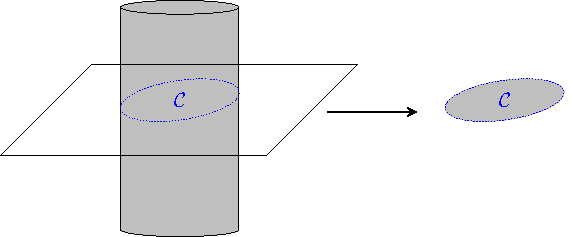
\includegraphics[width=0.8\textwidth]{passive/dimensionReduction.pdf}
 \caption[Schematic view of the reduction of Maxwell's equations from 3D to 2D]
	 {Our set of equations will be valid for infinitely long cylinders of
	  arbitrary cross-sections (shown on the left) and arbitrary physical parameters
	  $\epsilon$ and $\mu$. Our cavities, however, are bidimensional (shown on the right). 
	  The dimension reduction thus consists in postulating independence of the fields
	  and physical and geometrical parameters of the cavity with regards to the longitudinal coordinate 
	  and choosing a particular plane $\partial\Omega$.}
\end{figure}

To this effect, it will be useful to separate the field 
in transverse and longitudinal components. Following \cite{JAC1962,SCH2004b}, 
we suppose the fields can be written as 
  \begin{equation}
    \begin{Bmatrix}\bo{E}(\bo{r}_\perp,z)\\\bo{H}(\bo{r}_\perp,z)\end{Bmatrix} = \begin{Bmatrix}\bo{E}(\bo{r}_\perp)\\\bo{H}(\bo{r}_\perp)\end{Bmatrix}e^{i\beta z}
  \end{equation}
and we will also separate the fields and differential operators in two parts
  \begin{equation}
   \bo{E}(\bo{r}_\perp)= \bo{E}_\perp+E_z\bou{z}; \qquad \nabla=\nabla_\perp + \bou{z}\frac{d}{dz}.
  \end{equation}
Substitution in \eqref{eq:passive.formalism.generalCurlEquations} yields
  \begin{align}
    ik\mu H_z 		&= \left(\nabla_\perp\times\bo{E}_\perp\right)_z			& -ik\epsilon E_z 		&= \left(\nabla_\perp\times \bo{H}_\perp\right)_z	\label{eq:passive.formalism.longitudinalComponents}\\
    ik\mu\bo{H_\perp}	&= \left(-i\beta\bo{E}_\perp+\nabla_\perp E_z\right)\times\bou{z}	& -ik\epsilon\bo{E}_\perp 	&= \left(-i\beta\bo{H}_\perp+\nabla_\perp H_z\right)\times\bou{z} \label{eq:passive.formalism.tranverseComponents}
  \end{align}
The symmetry of these equations allow the decoupling of the tranverse and longitudinal components. 
Solving the system \eqref{eq:passive.formalism.tranverseComponents} 
shows that the scalar components $H_z$ and $E_z$ are the fundamental ones, 
as we can write the tranverse fields as a function of the longitudinal
ones:
  \begin{subequations}
  \begin{align}
    \bo{E}_\perp	&= \frac{i}{k^2n^2-\beta^2}\left[\beta\nabla_\perp E_z+k\mu\nabla_\perp H_z\times\bou{z}\right]	\\
    \bo{H}_\perp	&= \frac{i}{k^2n^2-\beta^2}\left[-k\epsilon\nabla_\perp E_z\times\bou{z}+\beta\nabla_\perp H_z\right].
  \end{align}
  \end{subequations}
Derivation of the differential equation for $E_z$ and $H_z$ can be
done via equations \eqref{eq:passive.formalism.longitudinalComponents}, but
is quite cumbersome. The details are thus not shown in this essay.

More specific boundary conditions can be derived with the use of these equations.
Applying the tranverse and longitudinal decomposition on \eqref{eq:passive.formalism.generalBoundaryConditions}
yields the six boundary conditions
  \begin{align*}
   E_{z1}		&= E_{z2}		& H_{z1}	&= H_{z2}	\label{eq:passive.formalism.contLongComponents}\\
   E_{t1}		&= E_{t2}		& H_{t1}	&= H_{t2}	\\
   \epsilon_1E_{n1}	&= \epsilon_2E_{n2}	& \mu_1H_{n1}	&= \mu_2H_{n2}
  \end{align*}
We seek to write the boundary conditions as a function of $H_z$ and $E_z$,
given that they are the fundamental fields. This can be done by taking
the projections of the transverse fields:
  \begin{subequations}
  \begin{align}
   E_t	&= \bou{t}\cdot\bo{E}_\perp = \frac{i}{\gamma^2}\left[\beta\partial_tE_z-k\mu\partial_nH_z\right]	\\
   E_n	&= \bou{n}\cdot\bo{E}_\perp = \frac{i}{\gamma^2}\left[\beta\partial_nE_z+k\mu\partial_tH_z\right]	\\
   H_t	&= \bou{t}\cdot\bo{H}_\perp = \frac{i}{\gamma^2}\left[k\epsilon\partial_nE_z+\beta\partial_tH_z\right]	\\
   H_n	&= \bou{n}\cdot\bo{H}_\perp = \frac{i}{\gamma^2}\left[-k\epsilon\partial_tE_z+\beta\partial_nH_z\right]	
  \end{align}
  \end{subequations}
where $\partial_{t,n}$ are the transverse and normal derivatives, respectively, and $\gamma^2=k^2n^2-\beta^2$.
Substituting these results in the boundary conditions for the transverse and normal components, we can 
derive the conditions $\partial_tE_{z1}=\partial_tE_{z2}$, $\partial_tH_{z1}=\partial_tH_{z2}$, which can 
shown to be equivalent to the continuity of the longitudinal components, 
\textit{viz.} \eqref{eq:passive.formalism.contLongComponents} \cite{SCH2004b}.
Combining all our previous results yields the four independent 
boundary conditions\index{boundary conditions!electromagnetic}:
  \begin{subequations}
  \label{eq:passive.formalism.cylindricalBoundaryConditions}
  \begin{align}
   E_{z1}	&= E_{z2}	\\
   H_{z1}	&= H_{z2}	\\
   \frac{k\mu_1}{\gamma_1^2}\frac{\partial H_{z1}}{\partial n}-\frac{k\mu_2}{\gamma_2^2}\frac{\partial H_{z2}}{\partial n} & = \beta\left(\frac{1}{\gamma_1^2}-\frac{1}{\gamma_2^2}\right)\frac{\partial E_{z1}}{\partial t}\\
   \frac{k\epsilon_1}{\gamma_1^2}\frac{\partial E_{z1}}{\partial n}-\frac{k\epsilon_2}{\gamma_2^2}\frac{\partial E_{z2}}{\partial n} & = -\beta\left(\frac{1}{\gamma_1^2}-\frac{1}{\gamma_2^2}\right)\frac{\partial H_{z1}}{\partial t}.
  \end{align}
  \end{subequations}
Notice that the propagation constant couples the electric 
and magnetic fields, regardless of the physical and geometrical
parameters of the cavity. 

\section{Scattering Matrix Formalism}
The previous section has provided us with the differential equations that 
we will need to solve to properly model bidimensional cavities. In this section, 
we will set up a scattering matrix (\gls{sMatrix}) formalism, augmented by the
time-delay matrix (\textit{\gls{qMatrix}})
that will allow us to quantify the response of the cavities
to an applied field and provide us with a novel way to determine their resonances. 
The numerical implementation of the method, being somewhat problematic, will 
be discussed at length. 

\subsection{$\mat{S}$ and $\mat{Q}$ Matrices Reloaded}
In dielectric cavities\index{dielectric resonators}, we need to solve the following equations
  \begin{multline}
    \left\{\nabla^2+k^2n^2\left[1-\left(\frac{\beta}{kn}\right)^2\right]\right\}\begin{Bmatrix} H_z \\ E_z \end{Bmatrix}
      = \frac{1}{1-\left(\frac{\beta}{kn}\right)^2}
	  \left[\frac{1}{\epsilon}\begin{Bmatrix} \nabla H_z \\ \nabla E_z \end{Bmatrix}\cdot\nabla\epsilon+\frac{1}{\mu}\begin{Bmatrix} \nabla  H_z \\ \nabla E_z \end{Bmatrix}\cdot\nabla\mu\right]
      \\-\begin{pmatrix} \frac{1}{\mu} & 0 \\ 0 &\frac{1}{\epsilon}\end{pmatrix} \begin{Bmatrix} \nabla H_z \cdot\nabla\mu \\ \nabla E_z\cdot\nabla\epsilon \end{Bmatrix}
      +\frac{\beta/kn}{1-\left(\frac{\beta}{kn}\right)^2}\left[\left(\sqrt{\frac{\mu}{\epsilon}}+\sqrt{\frac{\epsilon}{\mu}}\right)\begin{pmatrix}0 & -\frac{1}{\mu}\\\frac{1}{\epsilon} & 0\end{pmatrix}
      \begin{Bmatrix} \nabla H_z\times\nabla\mu \\ \nabla E_z\times\nabla\epsilon\end{Bmatrix}\right]
  \end{multline}
where $\beta$ is the propagation constant in the longitudinal direction.
Inhomogeneous cavities do not obey Helmholtz's equation like homogeneous
cavities do, but depend upon the first-order derivatives of the fields and 
physical properties of the medium. The two longitudinal fields
couple through the last term, where an anti-diagonal matrix appears.

%Modes with finite $\beta$ correspond, in the semiclassical limit, to
%rays that spiral up and down the cavity and refract out through 
%the caps \cite{TUR2005}. The cavity modes, the ones we are interested in, 
%are best modeled using $\beta=0$. 

In fact, this set of equations describe the propagation of light 
in optical fibers of arbitrary cross-section and arbitrary
refractive index profiles. However, we are interested in the modes
that are confined on a two-dimensional surface, the cavity modes. 
These modes must be independent of $z$ and we therefore take 
$\beta=0$. This is the main approximation of our model. It has been shown
to hold only approximately in experimental conditions \cite{DUB2008,BIT2010}, 
but we take the resulting equations to be the exact ones. This allows a 
simpler analysis for qualitative exploration; quantitative agreement
could be reached via perturbation methods or by using the integral method
we flesh out in Appendix \ref{sec:app.numTools.lippmannSchwinger}. This approximation 
has the much appreciated benefit of decoupling both the field
equations and the boundary conditions (see \eqref{eq:passive.formalism.cylindricalBoundaryConditions}).

Additionally exploiting the fact that we will only consider
non-magnetic media ($\mu=1$, $\epsilon=n^2$), our equation set becomes
  \begin{subequations}
  \label{eq:passive.formalism.fieldEquations}
  \begin{align}
    \left[\nabla^2+k^2n^2\right] H_z	&= \frac{2}{n}\nabla H_z\cdot\nabla n	\label{eq:passive.formalism.TEequation}\\
    \left[\nabla^2+k^2n^2\right] E_z	&= 0. 
  \end{align}
  \end{subequations}
In the following, it will be advantageous to form the field
$\bo{h}=\bo{H}/n$ \cite{DET2009}. This yields the equation
\cite{DET2009, GAP2013a}
  \begin{equation}
   \left[\nabla^2+k^2n^2-\frac{2\left(\nabla n\right)^2}{n^2}+\frac{\left(\nabla^2n\right)}{n}\right]h_z=0 \tag{\ref{eq:passive.formalism.TEequation}'}
   \label{eq:passive.formalism.TEequationPrime}
  \end{equation}
which is nothing but Helmholtz equation with an additional potential term.

\paragraph{The Quantum Connection}
Before putting forward the scattering formalism, it is interesting
to digress a little and explore the connection between the optical 
world and the quantum world. Specifically, the scalar version of
Maxwell's equations, the Helmholtz equations above, can be written 
as a Schrödinger equation
	\begin{equation}
		\left[\nabla^2+k^2\right]\psi = k^2\left(1-n^2(r,\theta)\right)\psi - V(\bo{r})
	\end{equation}
where $V(\boldsymbol{r})$  is the additional potential term just mentioned.
If the r.h.s. is such that equation is amenable to a solution by 
separation of variables, one obtains a radial potential of the form
	\begin{equation}
		V_\text{eff}(r) = k^2(1-n^2(r))+\frac{m^2-1/4}{r^2}-V(r).
	\end{equation}
For instance, the homogeneous, circular cavity yields a
potential as seen in Figure \ref{fig:passive.formalism.quantumConnection}. 
The jump at the boundary allows the existence of quasi-bound (QB) states\index{quasi-bound states} inside
the cavity, as opposed to bound states, as the light can tunnel outside the
potential barrier.

It is worth mentioning that the TM polarization behaves exactly has a 
quantum wavefunction does, the field and its normal derivative being
continuous at the interface, while the TE polarization is akin to 
a sonorous vibrations, as they may also obey ``jump'' conditions
at an interface \cite{COL2013}. Because of this, the TM polarization
is more present in the microcavities literature than the TE polarization.

\begin{figure}
	\centering
	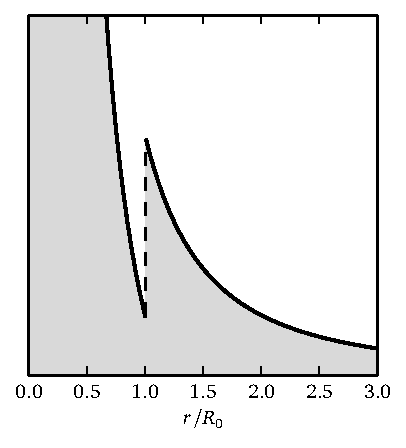
\includegraphics{figs/passive/quantumPotential.pdf}
	\caption[Effective radial potential associated with the homogeneous, circular cavity]
			{Effective radial potential associated with the homogeneous, circular cavity.
			We show the potential for $kR_0=5$, $m=10$ and $n_c=2$.}
	\label{fig:passive.formalism.quantumConnection}
\end{figure}

\begin{figure}
 \centering
 \def\svgwidth{0.4\textwidth}
 \input{figs/passive/dielectric.pdf_tex}
 \caption[Geometry of a bidimensional cavity]
	 {Geometry of a dimensional cavity. $R_0$ is the radius of the smallest circle
	 that encloses the physical microcavity, i.e. the last scattering surface. 
	 $R_V$ is the radius of a fictitious circle
	 that we will take to go to infinity.}
\label{fig:passive.formalism.geometry}
\end{figure}

We now return to the solution of the differential equations. 
We will adopt a scattering viewpoint. 
Imagine that the dielectric cavity is embedded in an infinite
medium of constant refractive index  $n_o=\sqrt{\epsilon\mu}$, 
as seen in Figure \ref{fig:passive.formalism.geometry}. 
Outside the cavity, $\bo{r}\not\in{\mathcal{C}}$, 
the r.h.s. of \eqref{eq:passive.formalism.fieldEquations} vanish. 
We call the surface that bounds the support of the function 
$n_o^2-n_c^2$ the \gls{lss}
The resulting equations are Helmholtz's and therefore have the well-known solution
  \begin{equation}
    \label{eq:passive.formalism.hankelSolution}
    \psi = \sum_{m} \left[A_m H_m^{(-)}(nkr) + B_m H_m^{(+)}(nkr)\right]e^{im\theta} \qquad (r>R_0).
  \end{equation}
where $H_m^{(\pm)}(z)$ are the Hankel functions of the first
and second kind. The Hankel functions are chosen in lieu of their
usual homologues $J_m(z)$ and $Y_m(z)$ as their asymptotic forms 
have incoming/outgoing cylindrical wave character, 
$H_m^{(\pm)}\propto \exp(\pm ikr)/\sqrt{r}$, thus ensuring that
the Sommerfeld radiation condition\index{Sommerfeld radiation condition} is fulfilled. The scattering
viewpoint essentially describes the relationship between the 
outgoing coefficients, $B_m$, and the incoming coefficients, $A_m$
via the \textit{scattering matrix}\index{scattering matrix}
  \begin{equation}
  	\label{eq:passive.formalism.defSmatrix}
    B_m = \sum_{m'}S_{mm'}A_{m'}. 
  \end{equation}
Much like its quantum-mechanical counterpart, the electromagnetic scattering
matrix can be interpreted as a phase shift acquired by the incoming
waves through interaction with the potential. This is most easily seen
by considering a central potential $V(r)$ where the \gls{sMatrix}
is diagonal. In that case, the $m$th component of the far-field can
be written as
  \begin{equation}
   \label{eq:passive.formalism.centralPotentialField}
   \psi_m^\text{FF} \propto \frac{1}{\sqrt{r}}\left[e^{-ikr}+e^{i\delta_m}e^{ikr}\right]
  \end{equation}
where we have written $S_{mm}=e^{i\delta_m}$ with $\delta_m\in\mathbb{R}$ 
as per the unitarity condition. The non-diagonal
generalization $S_{mm'}$ describes the coupling between angular
momenta $m\rightarrow m'$ and can be interpreted as a transition
probability.

When the \gls{sMatrix} is defined by the pair \eqref{eq:passive.formalism.hankelSolution}
and \eqref{eq:passive.formalism.defSmatrix}, it contains all near- and
far-field information. This is sharp contrast with the usual quantum 
scattering matrix, which is usually defined for a \gls{lss} having 
$r\rightarrow\infty$, i.e. in the far-field \cite{ROD1967,JOA1975,NEW1982}. In the scattering off dielectric structures, the potential 
$1-n^2$ has compact support in $\mathbb{R}^d$ and the \gls{lss} is taken to be 
a $(d-1)$-sphere containing the support of the potential.

In most applications (see the Introduction), we wish to find the \textit{resonances} of the
cavity. This is usually done by enforcing Sommerfeld radiation conditions
on Helmholtz's equation and looking for solutions of
  \begin{equation}
   \label{eq:passive.formalism.resonanceCondition}
   \mat{S}^{-1}\bo{B}=0;
  \end{equation}
for which a solution exists only if $|\det{\mat{S}(k)}|\rightarrow\infty$, 
i.e. at a pole of the \gls{sMatrix}. 
For real potentials, there cannot exist a solution on the real $k$ line because
of the flux conservation (unitarity) property of the \gls{sMatrix}. We 
must extend the search to the complex $k$ plane.

Equation \eqref{eq:passive.formalism.resonanceCondition} shows that the cavity 
\textit{creates} energy from nothing. In more physical terms, the cavity
has an infinite response to an infinitesimal energy input. This definition
of a resonance\index{resonance} implies that we should look in the $\Im{k}<0$ half-plane
for the poles of the \gls{sMatrix}. The solutions to this equation 
are known as QB states\index{quasi-bound states} as their intensity is usually larger
in the vicinity of the cavity and, contrary to their truly bound counterparts, 
have a small but non-zero value outside it. The ever so slowly decaying wavefunction
is thus non-normalizable (i.e. $\psi\notin L^2$). In this formulation, the field
has the following non-physical behaviour in the far-field
  \begin{align*}
   \psi_\text{FF}(\bo{r},t) 			&= \psi(\bo{r})e^{-i\omega t}	\\
						&\propto \exp\left[i(k'-ik'')r\right]\exp\left[-ic(k'-ik'')t\right]\exp[im\theta]	\\
   \left|\psi_\text{FF}(\bo{r},t)\right|^2 	&\propto e^{2k''r}e^{-2ck''t} 
  \end{align*}
where $k=k'-ik''$. The field thus exponentially increases with $r$, 
but exponentially \textit{decreases} with $t$. We can see, however, 
that the time scale of the exponential decrease is linked to the
imaginary part of the wavenumber by $\tau=\left(2ck''\right)^{-1}$.
We will use this relationship later in this essay.

It is interesting to note that the kind of resonances\index{resonance} supported
by dielectric cavities are of the same kind as those supported
by a forced, undamped harmonic oscillator. The incoming wave field
plays the part of the applied force. In the treatment of 
harmonic oscillators, it is usually noticed that adding a friction 
term in the equations curbs the infinities that the model otherwise 
yields. A parallel situation occurs in dielectric cavities. When there
is no absorption losses (friction), the response of the cavity 
to an incoming wave field is a result of the cumulative effect 
of the experimentally unattainable complex poles of the scattering matrix. 
However, when losses/gain are added into the model, the poles of the scattering
matrix begin to move in the complex plane; loss of unitarity implies that
it is possible that these poles may eventually move to the real $k$-line, 
making them experimentally feasible. This is in fact the backbone 
of the \gls{salt} \cite{GE2010a,GE2010b}.

Instead of directly looking for the poles, we will look for the signatures
of these poles on the real $k$ line by computing the \textit{energy}
of the modes and their complex coupling. This part of the formalism
was initially developed by G.P.-A. \cite{GAP2013a}: we will repeat
only what is necessary. 

Recall that the average electromagnetic energy of a field
in a given volume $V$
  \begin{equation}
   \mathcal{E}^V = \frac{1}{2}\mathop{\iiint}_V\left[\epsilon\bo{E}^*\cdot\bo{E}+\mu\bo{H}^*\cdot\bo{H}\right]d^3\bo{r}.
  \end{equation}
We form the energy matrix 
  \begin{equation}
   \mathcal{E}^V_{mm'} = \frac{1}{2}\mathop{\iiint}_V\left[\epsilon\bo{E}^*_m\cdot\bo{E}_{m'}+\mu\bo{H}^*_m\cdot\bo{H}_{m'}\right]d^3\bo{r}.
  \end{equation}
We will carry out the rest of the computation for the TM mode ($H_z=E_r=E_\theta=0$);
the argument holds for TE polarization \textit{mutatis mutandis} because of the
$k$-independence of the additional potential term in \eqref{eq:passive.formalism.TEequationPrime}
and also because $\bo{h}\propto\bo{H}$ for $r>R_0$. We thus have 
  \begin{align*}
    \bo{E}	&= \psi\bou{z}	\\
    \bo{H}	&= \frac{1}{ik}\nabla\times\bo{E}
  \end{align*}
and the energy matrix becomes
\begin{align}
    \mathcal{E}^V_{mm'}	&= \frac{1}{2}\mathop{\iiint}_V\left[\epsilon\psi^*_{m}\psi_{m'}+\frac{1}{k^2}\left(\nabla\times\psi_{m}\bo{\hat{z}}\right)\cdot\left(\nabla\times\psi^*_{m'}\bo{\hat{z}}\right)\right]d^3\bo{r}.	\nonumber\\
  \end{align}
Taking the parametric derivative of Helmholtz' equation, we get the 
following relations
  \begin{subequations}
  \label{eq:passive.formalism.parametricHelmholtz}
  \begin{align}
   \left[\nabla^2+n^2k^2\right]\psi								&=0	\\
   \left[\nabla^2+n^2k^2\right]\psi^*								&=0	\\
   \nabla^2\frac{\partial\psi}{\partial k}+2kn^2\psi+n^2k^2\frac{\partial\psi}{\partial k}	&=0
  \end{align}
  \end{subequations}
where we assume a real potential.
Forming the product\footnote{We use the identities \cite[Appendix II]{STR1941}
  \begin{equation*}
    \nabla\cdot\left(\phi\bo{A}\right) = \bo{A}\cdot\nabla\phi+\phi\nabla\cdot\bo{A}.
  \end{equation*}
and
  \begin{equation*}
    (\bo{a}\times\bo{b})\cdot(\bo{c}\times\bo{d}) = \bo{a}\cdot\left[\bo{b}\times(\bo{c}\times\bo{d})\right].
  \end{equation*}
}
  \begin{align*}
   \frac{1}{2k}\nabla\cdot\left[\frac{\partial\psi}{\partial k}\nabla\psi^*-\psi^*\nabla\frac{\partial\psi}{\partial k}\right]
	&= \frac{1}{2k}\left[\nabla\psi^*\cdot\nabla\frac{\partial\psi}{\partial k}+\frac{\partial\psi}{\partial k}\nabla^2\psi^*
			  -\nabla\frac{\partial\psi}{\partial k}\cdot\nabla\psi^*-\psi^*\nabla^2\frac{\partial\psi}{\partial k}\right]	\\
	&= \frac{1}{2k}\left[n^2\psi^*\left(2k\psi+k^2\frac{\partial\psi}{\partial k}\right)-\frac{\partial\psi}{\partial k}n^2k^2\psi^*\right]\\
	&= n^2\psi^*\psi
  \end{align*}
to write the energy matrix as
  \begin{align*}
    \mathcal{E}^V_{mm'} &= \frac{1}{4k}\int_V\nabla\cdot
			    \left\{
			      \frac{\partial\psi_{m'}}{\partial k}\nabla\psi^*_{m}-\psi^*_m\nabla\frac{\partial\psi_{m'}}{\partial k}
			+   \frac{2}{k}\left[\psi_{m'}\bo{\hat{z}}\times\nabla\times\psi^*_m\bo{\hat{z}}\right]\right\}d^3\bo{r}
  \end{align*}
Using the divergence theorem, noting that the normal vector
is the radial vector, we obtain
  \begin{align*}
    \mathcal{E}^V_{mm'}	&= \frac{wR_V}{4k}
			  \int_0^{2\pi}\left(\frac{\partial\psi_{m'}}{\partial k}\frac{\partial\psi^*_m}{\partial r}
					      -\psi^*_m\frac{\partial^2\psi_{m'}}{\partial k\partial r}\right)d\theta	\nonumber
			+\frac{wR_V}{2k}
			  \int_0^{2\pi}\psi_{m'}\frac{\partial\psi^*_m}{\partial r} d\theta
  \end{align*}
Using the exterior solution for $\psi_m$ and using the 
asymptotic expressions \eqref{eq:app.Bessel.asymptoticHankel} for the Hankel functions, we get
(after some algebra)
  \begin{align}
   \mathcal{E}^{\infty}_{mm'} &= \lim_{R_V\rightarrow\infty}\left[\frac{4n_0wR_V}{k}+\mathcal{O}(R_V^{-1})\right]\delta_{mm'}
			      + \frac{4w}{k}\left(-i\sum_\ell S^*_{\ell m}\frac{\partial S_{\ell m'}}{\partial k}\right)
  \end{align}
where $w$ is the thickness of the cavity. The first term is the 
diverging energy of the beam. Given that the incoming 
and outgoing waves are of infinite extent, this divergence
is only natural. The second term, however, depends only the
potential and can be interpreted as an excess energy due to the
cavity \cite{GAP2013a}. In matrix notation, we have
  \begin{equation}
  	\label{eq:passive.formalism.qMatrixDef}
    \mat{Q} = -i\mat{S}^\dagger\frac{d\mat{S}}{dk}.
  \end{equation}
This result coincides with the \gls{qMatrix} of quantum 
mechanics \cite{SMI1960}. The interpretation of this 
matrix is facilitated by \eqref{eq:passive.formalism.centralPotentialField}. 
Using the central potential, we can write
  \begin{equation}
    Q_{mm} = -ie^{-i\delta_m}\left(i\frac{\partial\delta_m}{\partial k}\right)e^{i\delta_m} = \frac{\partial\delta_m}{\partial k}.
  \end{equation}
The \gls{qMatrix} thus corresponds to the energy derivative of the 
phase shift, which has long been associated with the time-delay\index{time-delay}
introduced by the potential \cite{EIS1948,SMI1960,NUS1972,CAR2002,NUS1997,HAB2007}. 

The keen reader will have noticed that the above derivation
fails for complex potentials. The author has not found a proper
derivation for the extension to complex potentials. However, 
an expression can be found by this heuristic argument:
when the potential is complex, the phase shift $\delta_m$
becomes a complex function of $k$. In the preceding expression, 
we should take the inverse of the scattering matrix, not its Hermitian
transpose, to reproduce the energy derivative of the phase shift.
We thus have
  \begin{equation}
   \mat{Q} = -i\mat{S}^{-1}\frac{d\mat{S}}{dk}
  \end{equation}
as the proper generalization. This form was also used by Smith in
\cite{SMI1960}.
It is possible to arrive at this result with our derivation, but
with the extra term
	\begin{equation}
		-ik\mathop{\iint}_\mathcal{C}\Im{\epsilon(r,\theta)}\psi_m^*\frac{\partial\psi_{m'}}{\partial k}d^2\bo{r}
	\end{equation}
where $\mathcal{C}$ is the cavity region and the support of 
$\Im{\epsilon(r,\theta)}$. A similar result was obtained in 
\cite{MAR1975} where it was shown that this augmented \gls{qMatrix}
shares some properties of the Wigner-Smith time-delay matrix 
\eqref{eq:passive.formalism.qMatrixDef}. We will derive some of
these properties below. 

\subsection{Properties of the $\mat{S}$ and $\mat{Q}$ matrices}
The $\mat{S}$-matrix has multiple symmetries which can be used 
either to verify numerical implementations or to help tame 
numerical divergence issues. Most of the symmetries we will
expose in this thesis will concern the analytical continuation
of the scattering matrix in the complex $k$ plane. 

It is well known that the $\mat{S}$-matrix is unitary 
for real values of $n$ and $k$ \cite{NEW1982,LER2013}. However, 
it loses this important property is lost when we extend
to the complex plane \cite{MUG2004}. Looking at the complex conjugated versions
of our equation set, we see that we have
  \begin{align*}
    B_m		&= S_{mm'}(n,k)A_{m'}	\\
    A_m^*	&= S_{mm'}(n^*,k^*)B_{m'}^*
  \end{align*}
we can obtain the relation
  \begin{equation}
    \label{eq:passive.formalism.generalizedSmatrix}
    \mat{S}^{-1}(n^*,k^*) = \mat{S}^\dagger(n,k)
  \end{equation}
which reduces to the unitarity condition when 
the values are real. 

\begin{figure}
 \centering
 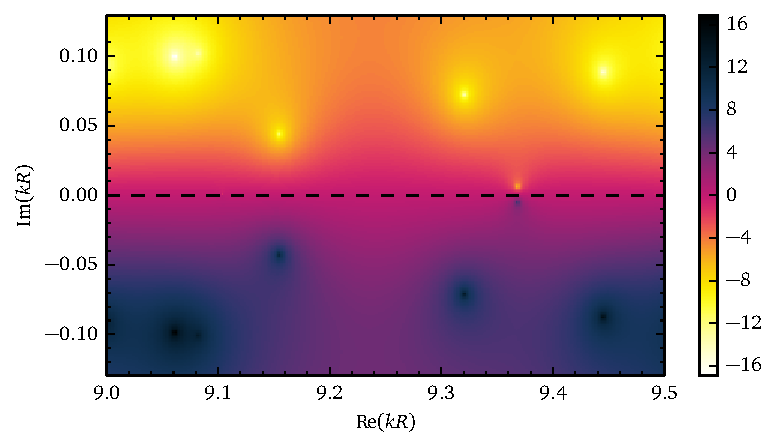
\includegraphics[width=0.8\textwidth]{figs/passive/determinantSmatrix.pdf}
 \caption[Mirror symmetry of the scattering matrix]
	 {Mirror symmetry of the scattering matrix. For this example, 
	 we computed $\log\left|\det\mat{S}(k)\right|$ for the scattering matrix of the
	 circular, homogeneous cavity with $n_c=3.2$ and $n_o=1$.}
  \label{fig:passive.formalism.symmetrySmatrix}
\end{figure}

Following \cite{GAP2013a}, we set up the following scattering
``experiment'':
  \begin{align*}
    H_m^{(-)}(z)e^{im\theta}					&\rightarrow \sum_{m'} S_{m'm}(n,k)H_{m'}^{(+)}(z)e^{im'\theta}	\tag{initial reaction}\\
    \sum_{m}S_{m'm}^*(n^*,k^*)H_m^{(-)}(z)e^{im\theta}		&\rightarrow H_{m'}^{(+)}(z)e^{im'\theta}			\tag{relation \eqref{eq:passive.formalism.generalizedSmatrix}}\\
    \sum_{m}S_{m'm}(n^*,k^*)\overline{H_m^{(-)}(z)}e^{-im\theta}&\leftarrow \overline{H_{m'}^{(+)}(z)}e^{-im'\theta}.		\tag{complex conjugate (time reversal)}
  \end{align*}
Use of \eqref{eq:app.Bessel.conjHankel}
leads to the relation, valid only when $k\in\mathbb{R}$
  \begin{equation}
    \label{eq:passive.formalism.timeReversalSymmetryReal}
    S_{m'm}(n,k) = (-1)^{m'}S_{-m-m'}(n^*,k)(-1)^m.
  \end{equation}
We can also write this in matrix form 
	\begin{equation}
		\mat{S}(n,k) = \mat{P}\mat{S}(n^*,k)^T\mat{P}
	\end{equation}
where $\left[\mat{P}\right]_{mm'} = (-1)^m\delta_{-mm'}$.
This relationship will be incredibly useful in the numerical implementation.

The \gls{qMatrix} also has some interesting properties. For real
potentials, it is Hermitian. This is a direct consequence of the
unitarity of the \gls{sMatrix} as 
  \begin{equation}
   \frac{d\mat{S}^\dagger\mat{S}}{dk} = \frac{d\mat{S}^\dagger}{dk}\mat{S}+\mat{S}^\dagger\frac{d\mat{S}}{dk} = 0
  \end{equation}
and
  \begin{equation}
   \mat{Q}^\dagger = i\frac{d\mat{S}^\dagger}{dk}\mat{S} = -i\mat{S}^\dagger\frac{d\mat{S}}{dk} = \mat{Q}
  \end{equation}
The delays associated with the potential are thus always real
and the delay eigenstates form a complete basis. Perhaps the
most interesting, and important, result concerning the 
\gls{qMatrix} is its connection with the complex poles of the
scattering matrix. It can be shown (see \cite{SHI2011,SHI2012,GAP2013a})
that we can seperate the scattering matrix in \textit{resonance channels} $\{\ket{p_j}\}$
and arrive at Simonius' form \cite{SIM1974}
  \begin{equation}
   \mathbf{S}(k)=\prod_{j=1}^\infty \mathbf{S}_j(k)
  \end{equation}
where
  \begin{equation}
   \mat{S}_j(k)\Ket{p_j} = \frac{k-k_j^*}{k-k_j}\Ket{p_j}.
  \end{equation}
Notice that this unitary expansion on the basis of the resonance
channels contains the mirror-symmetry of the poles and zeros of the 
scattering matrix. Figure \ref{fig:passive.formalism.symmetrySmatrix}
shows this symmetry in the case of the scattering matrix of the circular
disk. 

Using Simonius' expansion and the definition of the \gls{qMatrix}, we can obtain that
the eigendelays $q_p$ of each resonance channel have the form
  \begin{equation}
   \label{eq:passive.formalism.lorentzianDelays}
   q_p \propto \sum_j \frac{\Gamma_j}{\left(k-\Re{k_j}\right)^2-\Gamma_j^2/4}.
  \end{equation}
When the potential is real, it can be shown that 
	\begin{align}
		\mat{Q}\bo{A}^p	&= \tau_p\bo{A}^p &
		\mat{Q}\left(\mat{S}^\dagger\mat{P}\bo{A}^{p*}\right)	&=\tau_p\left(\mat{S}^\dagger\mat{P}\bo{A}^{p*}\right)
	\end{align}
share the same spectrum. Moreover, since $\mat{S}$ is unitary, we have 
$\left\|\mat{S^\dagger P}\right\|=1$ such that normalization is conserved. 
We can conclude that both sets of eigenvectors are related through a simple
phase factor such that
	\begin{equation}
		\left[\psi^p_\text{in}\right]^* = e^{-i\theta_p}\psi^p_\text{out}.
	\end{equation}
An interaction with a general potential changes the combination
of angular momenta of the incoming field (essentially the coefficients
of the Fourier-Bessel expansion, in our case) to a different one, 
forming a distinct outgoing field. The eigenvectors of the \gls{qMatrix}
form \textit{self-replicating modes}, as the interaction with the cavity
leave the angular momentum distribution unchanged and only phase shifts
the incoming wave. In turn, the energy derivative of this phase shift
gives information about the time-delay\index{time-delay} introduced 
by the interaction in the form of \eqref{eq:passive.formalism.lorentzianDelays}.

In the complex case, things become more complicated. Simonius' 
expansion is no more valid, as the poles and zeros are not 
longer symmetric along the real axis. The symmetry line
is shifted upward in the complex plane \cite{SAV2003,FYO2005}. 
Evaluating the \gls{qMatrix} along this line yields
a spectrum of real eigenvalues, referred to as the proper delay times. 
However, when the absorption is dispersive, the amount by which the symmetry
line depends on $\Re{k}$. We must thus evaluate the \gls{qMatrix} along
a curve in the complex $k$-plane. This shift depends non-trivially
on the absorption. It thus becomes rather hard to extract any meaningful
information for the \gls{qMatrix} for a general, complex, potential. 

\label{sec:passive.formalism.SpoleStructure}The \gls{sMatrix} also suffers some dramatic changes in its pole structure
\cite{JOF1973,KOK1981,CAS1982}, but the fact remains that the poles can still be
interpreted as the resonances of the cavity, and that the complex positions
yield information about the lifetimes of those resonances. Taking everything
into consideration, it seems that, for complex potentials, it is easier to 
work directly with the scattering matrix than to deal with the \gls{qMatrix}.

\section{Numerical Method I: SQA}
The numerical computation of the scattering matrix 
depends on two constructs: a polar discretization 
scheme colloquially denoted the onion discretization, and interior scattering matrices. We choose, for
the former, a rather standard radial discretization 
(see Fig. \ref{fig:passive.numerical.radialDiscretization}).
For easier reference, we dub the method \gls{sqa}.

\begin{figure}
 \centering
 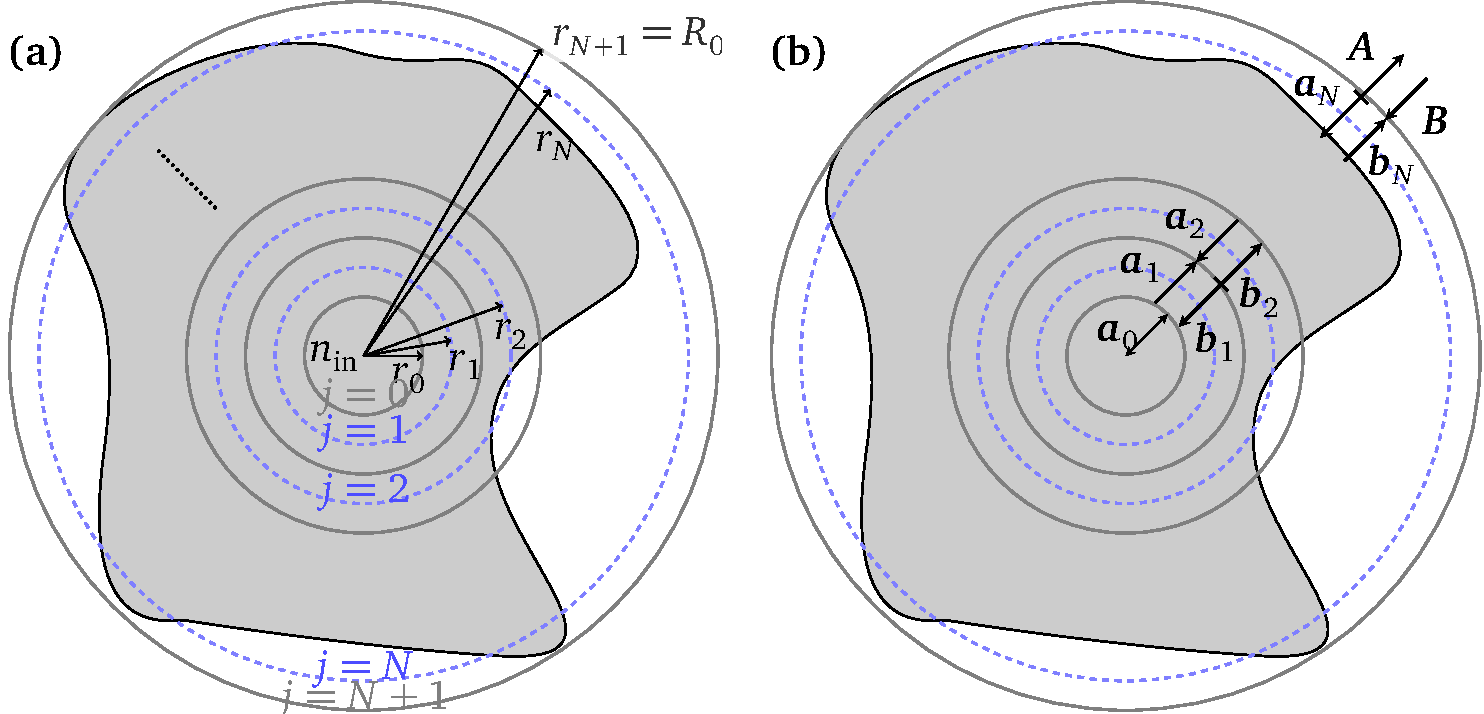
\includegraphics[width=0.9\textwidth]{figs/passive/figDisScatCoeff.pdf}
 \caption[Radial discretization for use in SQA]
	 {Radial discretization of the cavity for use in \gls{sqa}. The inner circle is assumed to 
	 have a constant refractive index denoted $n_\text{in}$. The full grey lines represent
	 the physical boundaries of each shell while the dotted blue lines represent their
	 center. \textbf{(a)} The central radius $r_j$ is the radial position at which the 
	 refractive index is sampled. Theh boundary conditions are enforced at $r=r_j\pm\epsilon$.
	 \textbf{(b)} Note the alternating propagation directions of the solutions inside each shell.
	 This reflects the local definition of ``incoming'' vs ``outgoing waves'' for each $r_j$.}
  \label{fig:passive.numerical.radialDiscretization}
\end{figure}

The latter relate the solutions
inside each radial shell to its neighboring shell. The final
interior scattering matrix relates the solution in the last shell
to the exterior solution, which is analytically known and is 
related to the \gls{sMatrix}\index{scattering matrix} of the cavity.

Our method is based on an algorithm originally developed by 
Rahachou and Zozoulenko \cite{RAH2004} and extended by \cite{GAP2013a}. 
We generalize the method to accept complex refractive index
profiles $n$.

\subsection{\textit{Divide et impera}}
We wish to solve the Hellholtz equation\footnote{The main text focuses on the
TM polarization; TE is treated in Appendix \ref{sec:app.numTools.scatMat}.}
  \begin{equation}
   \left[\nabla^2+k^2n^2\right]\psi = 0
  \end{equation}
inside the cavity. For $r>R_0$, the radius of the smallest circle
that encloses the whole dielectric, the solution is 
\eqref{eq:passive.formalism.hankelSolution}. We apply the discretization
of Fig. \ref{fig:passive.numerical.radialDiscretization}. We define a set of 
radii $\left\{r_j\right\}_{j=0}^{N+1}$ that denote the positions of the center
of the different shells. As such, $r_j-r_{j-1}=2\epsilon$ for the inner shells.
The cases $j=0$ and $j=N+1$ are different in that $r_0$ and $r_{N+1}$ denote 
the outer and inner limits of the domains, respectively. Moreover, $r_{N+1}-r_N=r_1-r_0=\epsilon\neq2\epsilon$.
As our first approximation, we suppose that the refractive index
inside the inner circle is constant and call it $n_\text{in}$. The Helmholtz equation then merely
becomes the Bessel equation \eqref{eq:app.Bessel.diffEquation}. Enforcing
finiteness of the field at $r=0$, we have the solution
  \begin{equation}
  	\label{eq:passive.formalism.innerCircleSoln}
   \Ket{\psi(r)} = \sum_{m}2a_m^0J_m(n_\text{in}kr)\Ket{\Phi_m^0}	\qquad (r<r_0)
  \end{equation}
where we have introduced bra-ket notation for the angular part of the 
solution. In that case, 
  \begin{equation}
   \Braket{\theta|\Phi_m^0} = e^{im\theta}.
  \end{equation}
In the shells $j>0$, the differential equation to solve is rather
  \begin{equation}
    \label{eq:passive.formalism.shellDiffEquation}
    \left[\frac{d^2}{dr^2}+\frac{1}{r}\frac{d}{dr}+\frac{1}{r^2}\frac{d^2}{d\theta^2}+k^2n^2(r,\theta)\right]\psi=0.
  \end{equation}
Inside each shell, we suppose that the potential strength depends only on the angular variable, i.e.
$k^2r^2n^2(r,\theta)\mapsto k^2r_j^2n^2(r_j,\theta)$ such that the angular sampling of the refractive
index is done at $r=r_j$ for each shell. \eqref{eq:passive.formalism.shellDiffEquation} 
is then amenable to a separation of variables
  \begin{subequations}
  \begin{align}
   \left[\rho_j^2\frac{d^2}{d\rho_j^2}+\rho_j\frac{d}{d\rho_j}-\xi^j\right]\mathcal{R}^j	&=0	\label{eq:passive.formalism.radialDiffEqn}	\\
   \left[\frac{d}{d\theta^2}+\left(k^2n^2(r_j,\theta)r_j^2+\xi^j\right)\right]\Phi^j		&=0
  \end{align}
  \end{subequations}
where $\rho_j=r/r_j$ is the scaled radial variable of the shell. 
These equations can readily be solved by noticing that
$\Phi^j(\theta+2\pi)=\Phi^j(\theta)$. We expand the solution
in a Fourier series
  \begin{equation}
   \Braket{\theta|\Phi_\mu^j} = \frac{1}{\sqrt{2\pi}}\sum_{m=-\infty}^\infty c_{m\mu}^je^{im\theta}
  \end{equation}
Projecting onto $\Ket{\Phi_m'^0}$ yields
\begin{equation}
    \sum_{m=-\infty}^\infty\left[-m^2\Braket{\Phi_{m'}^0|\Phi_m^j}+\xi^j\Braket{\Phi_{m'}^0|\Phi_m^j}+k^2r_j^2\Braket{\Phi_{m'}^0|n^2(r_j,\theta)|\Phi_m^j}\right]=0
  \end{equation}
Noticing that 
  \begin{equation}
    \Braket{\Phi_{m'}^0|\Phi_{m}^j} = \sum_{m=-\infty}^\infty c_{m\mu}^j \delta_{mm'}
  \end{equation}
we can write
  \begin{equation}
    \sum_m\left[-m^2\delta_{mm'}+\xi^j\delta_{mm'} + \frac{k^2r_j^2}{2\pi}\int_{0}^{2\pi}n^2(r,\theta)e^{i(m-m')\theta}d\theta\right]c_{m\mu}^j =0.
  \end{equation}
Using this last equation, we can set up an eigenvalue 
problem for the separation constant and the Fourier coefficients
  \begin{equation}
   \label{eq:passive.numerical.eigenvalue}
   \mat{L}^j\bo{c}_\mu^j=\xi_\mu^j\bo{c}_\mu^j
  \end{equation}
with
  \begin{equation}
    L_{mm'}^j = m^2\delta_{mm'}-\frac{k^2r_j^2}{2\pi}\int_0^{2\pi}n^2(r_j,\theta)e^{i(m-m')\theta}d\theta.
  \end{equation}
The particular form and additional properties of this matrix are discussed in 
Appendix \ref{sec:app.numTools.scatMat}.

Now that we know the set of eigenvalues $\{\xi_\mu^j\}$, we can solve the radial
equation \eqref{eq:passive.formalism.radialDiffEqn}. It is instantly recognized as 
a Cauchy-Euler equation. Given its coefficients, one can write the solution 
as \cite[p.~118-119]{GRE98}
  \begin{equation}
    \label{eq:sMatrix.radialSolution}
    \mathcal{R}_\mu^j(r) =  a_\mu^j\rho_j^{+\sqrt{\xi_\mu^j}}+b_\mu^j\rho_j^{-\sqrt{\xi_\mu^j}}.
  \end{equation}
  
Solving the $N$ eigenvalue problems \eqref{eq:passive.numerical.eigenvalue} gives
the solution in all space. We can now apply the boundary conditions \eqref{eq:passive.formalism.cylindricalBoundaryConditions}
at the interface of each shell $j\rightarrow j+1$. The process generates two sets of equations
  \begin{subequations}
  \label{eq:passive.numerical.boundaryCondition}
  \begin{align}
   \sum_\mu\left[a_\mu^j\rho_j^{+\sqrt{\xi_\mu^j}}+b_\mu^j\rho_j^{-\sqrt{\xi_\mu^j}}\right]\Ket{\Phi_\mu^j}
   &=
   \sum_\mu\left[b_\mu^{j+1}\rho_{j+1}^{+\sqrt{\xi_\mu^{j+1}}}+a_\mu^{j+1}\rho_{j+1}^{-\sqrt{\xi_\mu^{j+1}}}\right]\Ket{\Phi_\mu^{j+1}}	\\
   \frac{d}{dr}\sum_\mu\left[a_\mu^j\rho_j^{+\sqrt{\xi_\mu^j}}+b_\mu^j\rho_j^{-\sqrt{\xi_\mu^j}}\right]\Ket{\Phi_\mu^j}
   &=
   \frac{d}{dr}\sum_\mu\left[b_\mu^{j+1}\rho_{j+1}^{+\sqrt{\xi_\mu^{j+1}}}+b_\mu^{j+1}\rho_{j+1}^{-\sqrt{\xi_\mu^{j+1}}}\right]\Ket{\Phi_\mu^{j+1}}
  \end{align}
  \end{subequations}
The interior scattering matrices
are constructed via pre-multiplying by the left eigenvectors\index{left eigenvectors} $\Bra{\tilde{\Phi}_\mu^j}$ on each side. 
Combining both resulting equations leads to the linear system 
  \begin{equation}
    \begin{pmatrix}\mat{A} & \mat{B} \\ \mat{C} & \mat{D} \end{pmatrix} \begin{pmatrix} \bo{a}^j \\ \bo{a}^{j+1}\end{pmatrix}
    =
    \begin{pmatrix}\mat{E} & \mat{F} \\ \mat{G} & \mat{H} \end{pmatrix} \begin{pmatrix} \bo{b}^j \\ \bo{b}^{j+1}\end{pmatrix}
  \end{equation}
which can be inverted using Schur's complements\index{Schur complements} \cite[p.~123]{MEY2001} to yield a relationship between the 
$\bo{a}$ and $\bo{b}$ coefficients, i.e.
  \begin{equation}
   \mat{S}_j = \begin{pmatrix}\mat{E} & \mat{F} \\ \mat{G} & \mat{H} \end{pmatrix}^{-1}\begin{pmatrix}\mat{A} & \mat{B} \\ \mat{C} & \mat{D} \end{pmatrix}.
  \end{equation}
Physically, the $\mat{S}_j$ matrix relates the locally 
incoming waves from shell $j+1$ in shell $j$ to the locally 
outgoing from shell $j$ to shell $j+1$. The last necessary
breakthrough is to realize that we can connect the solutions
from shell $j$ to those of the shell $j+2$, then $j+3$ and 
so on. When started from $j=0$, this iterative process yields
the relationship
  \begin{equation}
   \begin{pmatrix}\bo{a}^0\\\bo{B}\end{pmatrix} = \mat{S}^{0,N}\begin{pmatrix}\bo{a}^0\\\bo{A}\end{pmatrix}
  \end{equation}
such that the \gls{sMatrix} of the system is
the block $\mat{S}_{22}^{0,N}$. More details can be found
in Appendix \ref{sec:app.numTools.scatMat}. 
  
\subsection{Numerical Analysis and Calibration}
While numerical analysis has been heavily formalized in recent years, 
it is still as much an art as a science. In implementing the algorithm, 
we thus came across two potential problems: the inversion of the 
$\mat{K}$ matrix (defined below) and the final Hadamard product
$\mathcal{H}\circ\mat{S}^{0,N}_{22}$. We analyze the two issues
and provide solutions to the instabilities they cause. We also 
calibrate the method with systems whose analytical solution
is known: the homogeneous circular cavity and the annular cavity.
We also compare our method to results obtained in the literature. 

\subsubsection{Numerical Back and Forth}
For the computation of each $\mat{S}_j$, we must invert
a matrix of the form 
  \begin{equation}
  \mat{K}^{j,j+1} = \left(\frac{r_j-\epsilon}{r_j+\epsilon}\right)^{\bo{\Lambda}^j}
		    -\tilde{\mat{S}}^{j+1}_{11}\left(\frac{r_j+\epsilon}{r_j-\epsilon}\right)^{\bo{\Lambda}^j}\tilde{\mat{S}}^{0,j}_{22}.
  \end{equation}
Given that the elements of this matrix highly depend upon the discretization
parameter $\epsilon$, the half-width of the shells, we can use the
condition number $W$ of this matrix as an indicator of the quality
of the discretization. It can be grossly estimated by the 
ratio of the maximum and minimum elements of the matrix. 
By assuming that there is no amplification in the system,
all interior scattering matrices have
$||\mat{S}||\leq1$ and we can approximate
  \begin{equation}
   W \sim \left(\frac{r_j+\epsilon}{r_j-\epsilon}\right)^{2\lambda_\text{max}}\sim 1 + \frac{4\lambda_\text{max}\epsilon}{r_j}
  \end{equation}
according to the binomial expansion.
To evaluate the $\lambda_\text{max}$ parameter, we will
have to take a detour and introduce the concept 
of \textit{\glspl{gerschgorin}} and some obscure
properties of Fourier series.

\paragraph{Gerschgorin Circles}
Gerschgorin circles provide a way to bound the spectrum 
of square matrices by simply examining its entries.

\begin{thm}[Gerschgorin circles \protect{\cite[p.~498]{MEY2001}}]
 The eigenvalues of a matrix $\mat{A}\in\mathbb{C}^{n\times n}$ are
 contained within the intersection $\mathcal{G}_r\cap\mathcal{G}_c$
 of the sets of row and column Gerschgorin circles, defined respectively as
  \begin{align*}
   \mathcal{G}_r	&= \left\{|z-a_{ii}| \leq \sum_{\stackrel{j=0}{j\neq i}}^{n-1} |a_{ij}|; \quad \forall i\right\}
  & \mathcal{G}_c	&= \left\{|z-a_{jj}| \leq \sum_{\stackrel{i=0}{i\neq j}}^{n-1} |a_{ij}|; \quad \forall j\right\},
  \end{align*}
 or, in a slightly more algorithmically-friendly form:
  \begin{equation}
   \mathcal{G}_r\cap\mathcal{G}_c = \left\{|z-a_{ii}| \leq \min\left(\sum_{\stackrel{j=0}{j\neq i}}^{n-1} |a_{ij}|,\sum_{\stackrel{j=0}{j\neq i}}^{n-1} |a_{ji}|\right)
				     ;\quad \forall i\right\}.
  \end{equation}
\end{thm}

\begin{corr}\label{corr:passive.numerical.diagDominantMatrices}
 Diagonally dominant matrices are non-singular.
\end{corr}

 \begin{proof}
  Diagonally dominant matrices, by definition, have 
    \begin{equation}
     |a_{ii}| > \max\left(\sum_{\stackrel{j=0}{j\neq i}}^{n-1} |a_{ij}|, \sum_{\stackrel{j=0}{j\neq i}}^{n-1} |a_{ji}|\right)
    \end{equation}
  and, by Gerschgorin's theorem, do not have 0 as an eigenvalue, $0\notin\sigma(\mat{A})$, and therefore are 
  non-singular.
 \end{proof}

\begin{exmp}
  Consider the matrix \cite[p.~499]{MEY2001}
  \begin{equation}
    \label{eq:passive.numerical.exampleMatrixGerschgorin}
    \mat{A} = \begin{pmatrix} 5 & 1 & 1 \\ 0 & 6 & 1 \\ 1 & 0 & -5 \end{pmatrix}.
  \end{equation}
  Its associated Gerschgorin circles are shown in Figure \ref{fig:passive.numerical.gerschgorinCircles}. 
  We see that the row and column circles give different bounds on the eigenvalues and their intersection 
  yields the best possible approximations for the eigenvalues. 
\end{exmp}

\begin{figure}
 \begin{subfigure}{\textwidth}
  \centering
  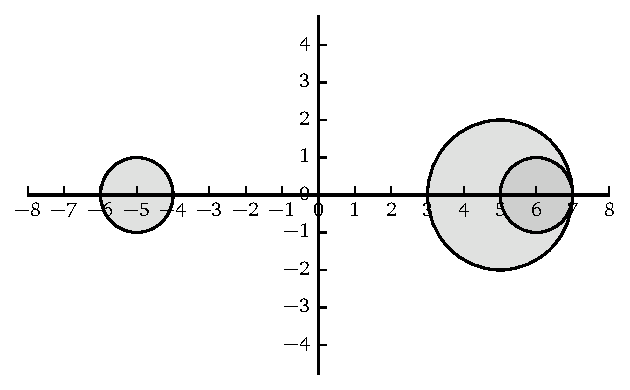
\includegraphics{figs/passive/gerschgorin-row.pdf}
  \caption{Row Gerschgorin circles}
 \end{subfigure}
 
 \begin{subfigure}{\textwidth}
  \centering
  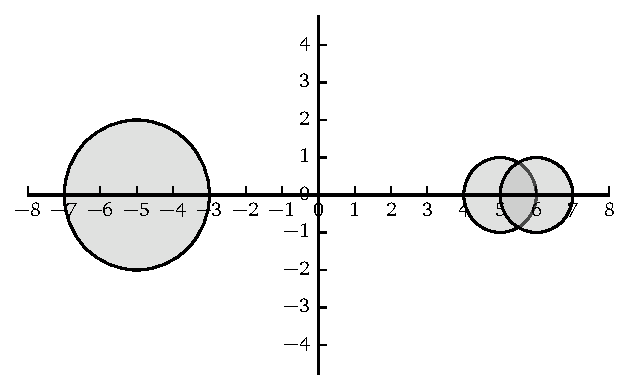
\includegraphics{figs/passive/gerschgorin-col.pdf}
  \caption{Column Gerschgorin circles}
 \end{subfigure}
 
 \begin{subfigure}{\textwidth}
  \centering
  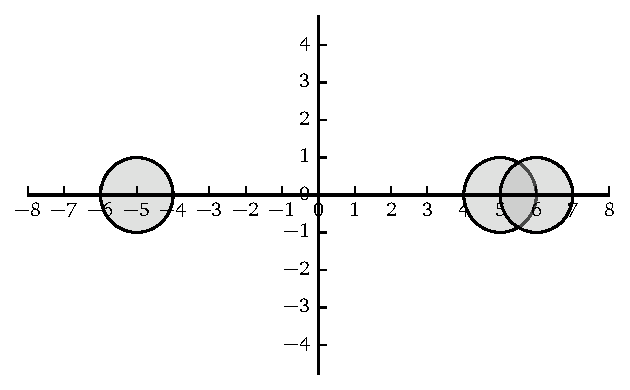
\includegraphics{figs/passive/gerschgorin-full.pdf}
  \caption{Intersection of both previous sets}
 \end{subfigure}
 \caption[Gerschgorin circles for an example matrix]
	 {Gerschgorin circles of the matrix defined in \eqref{eq:passive.numerical.exampleMatrixGerschgorin}.
	 Notice that the matrix is non-singular by Corrolary \ref{corr:passive.numerical.diagDominantMatrices}.}
 \label{fig:passive.numerical.gerschgorinCircles}
\end{figure}

We now apply the Gerschgorin circles to our $\mat{L}^j$ matrix. 
In Appendix \ref{sec:app.numTools.scatMat}, we show that a proper choice for $M$
is $M=2kR_0\sqrt{\mathop{\max}_{(r,\theta)}\left(n^2(r,\theta)\right)}$. This criterion
ensures that we sample the refractive index above the Nyquist frequency\index{Nyquist frequency}. The largest
diagonal element (the farthest Gerschgorin circle) corresponds
to the highest angular momentum and has a magnitude of 
$4k^2R_0^2\mathop{\max}_{(r,\theta)}\left(n^2(r,\theta)\right)-k^2R_0^2n^2(r,\theta)\sim3k^2R_0^2n^2$.
The radius is more complicated to estimate, as it is given by the sum of the norm
of the Fourier coefficients of $n^2(r,\theta)$, which we call $n_m$:
  \begin{equation}
   r = \sum_{m=1}^M |n_m|.
  \end{equation}
It can be shown that there exists an upper bound for the value of the
Fourier coefficients \cite{JAC1920}
  \begin{equation}
   |n_m| \leq \frac{V}{2m\pi}
  \end{equation}
where $V$ is the variation of the refractive index and is define as
  \begin{equation}
   V(r) = \int_0^{2\pi}\left|\partial_\theta n^2(r,\theta)\right|d\theta.
  \end{equation}
To go further, we must realize the mixed blessing of the logarithmic
divergence of the harmonic series\footnote{A better bound could be obtained, but requires conditions
on the behaviour $n^2(r,\theta)$ that the author is not comfortable assuming.}. We estimate the radius
of the Gerschgorin circle by taking $M=500$, an arbitrary bound
that is unattainable by our algorithm\footnote{The Bessel functions overflow our floating representation at approximately $M\sim250$,
rendering the algorithm useless.}
such that the upper bound for the radius becomes $r\leq 3V/\pi$. Taking the annular
cavity as an example, the variation is approximately given by 
$2n^2$. Pulling everything together, this yields an approximate upper
bound for the largest eigenvalue as
  \begin{equation}
   |\lambda_\text{max}| < 3nkR_0
  \end{equation}
A good choice of $\epsilon$ is thus
  \begin{equation}
   \epsilon \ll \frac{1}{12nk} \ll \frac{\lambda}{2n}
  \end{equation}
which mirrors the conventional wisdom. This empirical rule
is applied in every computation in this essay.

\subsubsection{Hadamard Product}
Like Frodo before Mount Doom, we must face a final challenge
before conquering upon all evil, or, in our case, computing
the scattering matrix. Our final demon
takes the form of the product
  \begin{equation}
   \mat{S} = \left[\mat{H}^{(+)}\right]^{-1}\mat{S}^{0,N}_{22}\mat{H}^{(-)}
  \end{equation}
where the $\mat{H}$ are diagonal matrices with entries $H_m^{(\pm)}(n_okR_0)$. 
We recast the matrix product as a Hadamard (element-wise) product
 \begin{equation}
  \mat{S} = \mathcal{H}\circ\mat{S}^{0,N}_{22}
 \end{equation}
with $\mathcal{H}_{mm'} = H_m^{(-)}(n_okR_0)/H_{m'}^{(+)}(n_okR_0)$.
A quick peek at Fig. \ref{fig:passive.numerical.hankelHadamard} 
announces the disaster. The region $|m'|>|m|$ increases 
exponentially with $|m'|-|m|$. This wouldn't be an issue 
if the corresponding elements of the block scattering
matrix $\mat{S}^{0,N}_{22}$ were exponentially decreasing (as
we physically expect them to); however, the numerical construction
of this matrix implies the addition and subtraction of $\mathcal{O}(1)$
floating-point numbers, limiting their range to about $10^{-15}$, the decimal
accuracy associated with \texttt{double} precision arithmetic. Consequently, 
the final Hadamard product yields scattering matrices with unphysically
large off-diagonal elements.

\begin{figure}
 \centering
 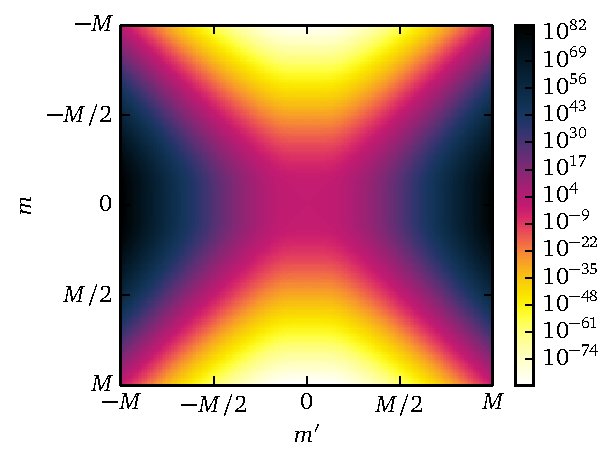
\includegraphics{figs/passive/absHadamard.pdf}
 \caption[General form of absolute value of the Hankel matrix $\mathcal{H}$]
	 {General form of absolute value of the Hankel matrix $\mathcal{H}$.
	 We have used the parameters $z=10$ and $M=100$, but
	  the pattern scales with $M$ and $z$.}
 \label{fig:passive.numerical.hankelHadamard}
\end{figure}

Several solutions to this numerical artefact have been considered, e.g. the use of matrix masks
and of higher precision arithmetic. The latter was swiftly abandoned
due to the difficulty of the implementation\footnote{Even if we disregard
the fact that no C++ compiler support the IEEE 754 \texttt{binary128}
quadruple precision float-point representation, we would still need
to find numerical libraries that extend the BLAS and LAPACK libraries
to work at higher precision.}, even though it could help stabilize the
numerical algorithm \cite[\S 5.8.4]{MIS2002}. The use of matrix masks is 
made possible by noting that the cavity cannot convert arbitrarily
high angular momenta. The maximum angular momentum it can affect, 
$M_\text{max}$ is a function of its ``degree of inhomogeneity'', 
characterized by the absolute size of the Fourier components
of the refractive index (which also depends on the geometry
of the cavity). This gives the \gls{sMatrix} a banded form 
(see Fig. \ref{fig:passive.numerical.bandedFormSmatrix} for
an example using the elliptical cavity). The width of
this band could be detected in $\mat{S}^{0,N}_{22}$ before
taking the Hadamard product, or inferred from the coefficients
of the Fourier transform of $n^2(r,\theta)$. After the product, all elements
outside this band could be set to zero. The interested 
reader might want to go through Türeci's discussion of
the banded form and the numerical problems associated 
with the Hankel matrices \cite[\S 3.4]{TUR2003}.

\begin{figure}
 \centering
 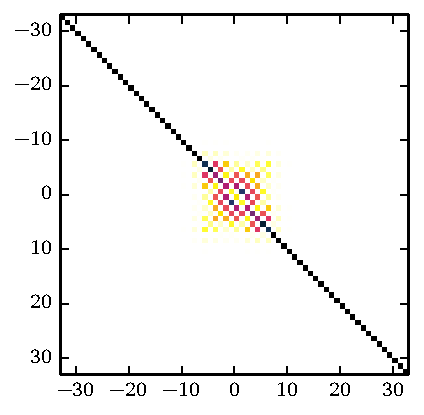
\includegraphics{figs/passive/sMatrixEllipseMag.pdf}
 \caption[Banded form of the scattering matrix of the elliptical cavity]
	 {Scattering matrix of the elliptical cavity with $n_c=3.3$, $a=1$
	 and $b=0.53477$, giving $e=0.845$. Recall that $r(\theta)=ab/\sqrt{(b\cos\theta)^2+(a\sin\theta)^2}$.
	 Notice that the non-vanishing elements have a banded form: they decrease with the distance
	 from the diagonal and eventually go to zero. Beyond a particular value of the angular momentum 
	 ($M_\text{max}=6$, in this case), the scattering matrix is diagonal: there is no mixing of angular momenta.
	 The value of $M_\text{max}$ depends on the inhomogeneity of both the boundary of the cavity and that of its
	 refractive index. It could be inferred from the Fourier transform of the refractive index.}
 \label{fig:passive.numerical.bandedFormSmatrix}
\end{figure}

We have, however, chosen a different path. 
It turns out that relation \eqref{eq:passive.formalism.timeReversalSymmetryReal}
precisely relates the diverging parts of the Hankel matrix
to its vanishing one. Imposing this symmetry on the numerical scattering
matrix allows the algorithm to return physical scattering matrices. 
This limits the scope of our method to real energies ($k$) and has a
high computational cost for complex refractive indices. This limitation, 
coupled to the fragility of the generalization to $n\in\mathbb{C}$\footnote{
We discuss this fragility in more detail in Appendix \ref{sec:app.numTools.scatMat}.} suggests
the use of other methods for complex energies and potentials.

\subsubsection{Calibration}
One of the most important step in algorithmic creation
is the \textit{\gls{calPhase}}. We calibrate the method
using the analytical form of the \gls{sMatrix} for the
homogeneous, circular cavity and compare the results 
from the literature. 

\paragraph{Homogeneous, Circular Cavity}
The scattering matrix of the homogeneous circular cavity
is trivially obtained. Assuming that the refractive index inside
the cavity is $n_c$ and $n_o$ outside, the solution inside the 
cavity is given by 
  \begin{equation}
   \psi^c = \sum_m a_m^cJ_m(n_okr)e^{im\theta}
  \end{equation}
while the solution outside the cavity is given by \eqref{eq:passive.formalism.hankelSolution}.
Imposing the electromagnetic boundary conditions yields two infinite sets of equations
for three sets of coefficients. Solving yields a linear relationship between the 
$A_m$ and $B_m$ sets, \textit{viz.} the scattering matrix
  \begin{equation}
   \label{eq:passive.numerical.sMatrixHomo}
   S_{mm'}^\text{HD} = -  \frac{\eta_{co}J_m'(Z_c)H_m^{(-)}(Z_o)-J_m(Z_c){H^{(-)}_m}'(Z_o)}
				{\eta_{co}J_m'(Z_c)H_m^{(+)}(Z_o)-J_m(Z_c){H^{(+)}_m}'(Z_o)}\delta_{mm'}.
  \end{equation}
where $Z_c = n_ckR_0$, $Z_o=n_okR_0$ and $\eta_{co}= n_c/n_o\; (n_o/n_c)$ in TM (or TE) polarization.

Before, we showed the correspondence between the poles of the scattering matrix and its associated
time delay spectrum analytically (see p.~\pageref{eq:passive.formalism.lorentzianDelays}). 
In Fig.~\ref{fig:passive.numerical.correspondanceRoots}, we show the
time delay spectrum of the homogeneous disk. The corresponding poles of the \gls{sMatrix} are denoted
by squares\footnote{The poles are computed via the zeros of the denominator of \eqref{eq:passive.numerical.sMatrixHomo}
using a Newton-Raphson algorithm. The initial guesses are provided by the asymptotic ($kR_0\gg m$) zeros
of the denominator. See \cite[Annexe A.2.4]{GAG2011} for a derivation.}. There seems to be a problem with the very high-$Q$ ones, but this is only due to the fact
that we have not used a proper discretization $\Delta k$. The other ones line up perfectly with the peaks
of the time delay. 

In Fig.~\ref{fig:passive.numerical.convergenceHomogeneousDisk}, we compare the analytical scattering
matrix to the one computed via SQA. We use 
  \begin{equation}
   E = \max\left[\mat{S}_\text{ana}-\mat{S}_\text{SQA}\right] 
  \end{equation}
as a function of the discretization size $kR_02\epsilon$ to measure
the error. Notice that the convergence speed is the same for all curves, 
regardless of the value of $kR_0$. Convergence does not depend on the value of $M$
as the homogeneous, circular cavity has a diagonal scattering matrix. 

\begin{figure}
  \centering
  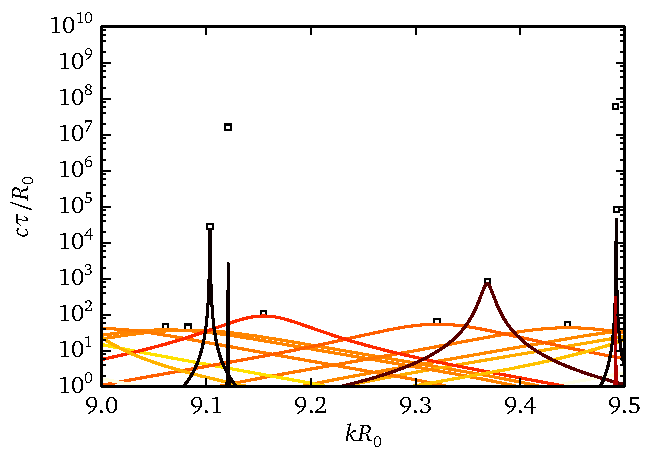
\includegraphics[width=0.8\textwidth]{figs/passive/correspondanceRootsPeaks.pdf}
  \caption[Correspondence between the poles of the scattering matrix and the peaks
	  of the time delay spectrum.]
	  {Time delay spectrum of a circular cavity with $n_c=3.2$ and $n_o=1$ in TM polarization. The squares
	  represent the complex position of the poles of the scattering matrix. The equivalent
	  time delay is computed using $c\tau/R_0=-\Re{kR_0}/2\Im{kR_0}$.}
  \label{fig:passive.numerical.correspondanceRoots}
\end{figure}


\begin{figure}
 \centering
 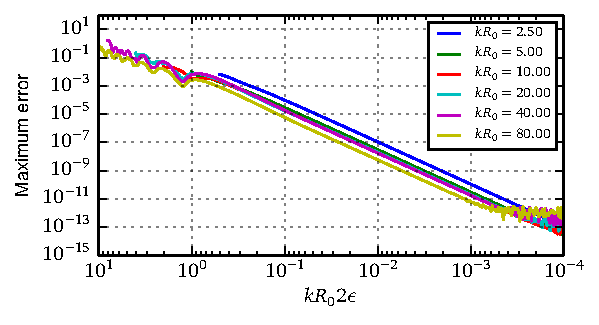
\includegraphics{figs/passive/convergenceHomo.pdf}
 \caption[Convergence properties of SQA when applied on the homogeneous disk]
	  {Calibration of \gls{sqa} against the homogeneous disk. The cavity 
	  has refractive index $n_c=1.5$ and is embedded in air $n_o=1$. The exterior
	  radius is set to $R_0=1$ and we take the number of shells to be $N=2$.
	  The error approximately follows a cubic power-law behaviour in the discretization
	  size.}
 \label{fig:passive.numerical.convergenceHomogeneousDisk}
\end{figure}

%\paragraph{Annular Cavity}
%The annular cavity is a circular cavity with constant refractive index
%profile in which a circular hole has been cut, see Fig. \ref{fig:passive.numerical.annularCavityGeometry}
%for a picture. 
%Derivation of the scattering matrix of the annular cavity is a little
%more involved. Suffice it to say that it is given by 
%  \begin{equation}
%   \mat{S}^\text{AC} = -\left[n_o{\mat{H}^{(-)}}'(Z_o)-n_c\mat{H}^{(-)}(Z_o)\mat{GF}^{-1}\right]
%			\left[n_o{\mat{H}^{(+)}}'(Z_o)-n_c\mat{H}^{(+)}(Z_o)\mat{GF}^{-1}\right]^{-1}
%  \end{equation}
%where 
%  \begin{align}
%   \mat{F} &= \mat{H}^{(-)}(Z_c)+\mat{H}^{(+)}(Z_c)\mat{S}^\text{HD} & \mat{G} = {\mat{H}^{(-)}}'(Z_c)+{\mat{H}^{(+)}}'(Z_c)\mat{S}^\text{HD}.
%  \end{align}
%A proper derivation can be found in \cite{HEN2002b}; an improved
%one can be found in \cite[Appendix D]{GAP2013a}.
%
%\begin{figure}
%  \begin{center}
%  \begin{tikzpicture}[scale=3]
%   % -- Draw basic geometry
%   \draw[very thick,fill=gray!30!white] (0,0) circle (1);
%   \draw[very thick,fill=white] (0.35,0.35) circle (0.25);
%  
%   % -- Draw coordinate systems and distances.
%   % Center line.
%   \draw[dash pattern=on 5pt off 2pt,thick] (-1,0) -- (1,0);
%   
%   % Coordinates of big cavity.
%   \draw[->,>=stealth,thick] (0,0) -- (-0.5,0.5) node[above left] {$r$};
%   \draw (0.1,0) arc (0:135:0.1) node[midway,above] {$\theta$};
%   
%   % Radius of big cavity.
%   \draw[->,>=stealth,thick] (0,0) -- (-0.96,-0.2588) node[near end,below] {$R_0$};
%   
%   % Center lines for inclusion.
%   \draw[dash pattern=on 5 pt off 2pt, gray] (0.1,0.35) -- (0.6,0.35);
%   \draw[dash pattern=on 5 pt off 2pt, gray] (0.35,0.1) -- (0.35,0.6);
%   
%   % Coordinates of inclusion w/r to big cavity.
%   \draw[->,>=stealth,thick,BurntOrange] (0,0) -- (0.35,0.35) node[near end, above] {$d$};
%   \draw[BurntOrange] (0.15,0) arc (0:45:0.15) node[midway,right] {$\Theta$};
%  \end{tikzpicture}
%  \end{center}
%  \caption[Geometry of the annular cavity]
%	  {Geometry of the annular cavity. The circular cavity has coordinate system
%	  $(r,\theta)$ and radius $R_0$ Its refractive index is denoted by $n_c$. 
%	  The circular inclusion has position $\color{BurntOrange}(d,\Theta)$
%	  in the main coordinates and its refractive index is $n_h$. It isually is the same
%	  as $n_0$, the refractive index of the environment.}
%  \label{fig:passive.numerical.annularCavityGeometry}
%\end{figure}
%
%
%\todo[inline]{Calibration with annular cavity.}

\paragraph{Comparison to other methods}
To make sure we can blindly accept the results of our numerical
technique, we apply it to non-integrable geometries that have been
studied by other means in the literature. Table \ref{tab:passive.numerical.comparisonLiterature}
shows a comparison of the positions of the certain resonances 
for a set of selected geometries. Fig. \ref{fig:passive.numerical.squareSpectrum}
shows the time delay spectrum of the square cavity. The higher-delay mode, 
highlighted in the figure, has a field profile (inset) that resembles
a WGM. The localization of light in square cavities has since been 
confirmed experimentally \cite{BIT2013} and observed in other geometries
\cite{SON2013}.

We also notice that the resonance at $k=4.53$ is degenerate. The highlighted
mode has a high delay, but it coexists with a low delay mode. In practice, when
there are imperfections, this might become a problem, as the high-$Q$ modes
are highly sensitive to perturbations \cite{RAH2004}. Another interesting
feature can be seen at $k\sim4.545$, where two modes show an avoided
crossing. The vertical line the spectrum corresponds to where the modes
``switch''. 

\begin{table}
  \newcolumntype{d}{D{.}{.}{3}}
  \begin{tabular*}{\columnwidth}{l@{\extracolsep{\fill}}ddddc}
  \hline\hline
  \multirow{2}{*}{Cavity}	& \multicolumn{2}{c}{SQA}					& \multicolumn{2}{c}{Emission Viewpoint}				& \multirow{2}{*}{Source}	\\
				& \multicolumn{1}{c}{$kR_0$}	& \multicolumn{1}{c}{$2R_0/c\tau$}	& \multicolumn{1}{c}{$\text{Re}\{kR_0\}$}&\multicolumn{1}{c}{$|\text{Im}\{kR_0\}|$}	&\\
\hline\hline
  Square			& 4.53				& \multicolumn{1}{c}{$1.06\times10^{-4}$}& 4.54					&\multicolumn{1}{c}{$1.05\times10^{-4}$}&\cite{GUO2003}\\
  Stadium			& 4.89				& 0.052					& 4.89					&0.055					&\cite{LEE2004}\\
  Ellipse			& 6.499				& 0.029					& 6.50					&0.032					&\cite{UNT2008}\\
  Annular			& 10.266			& 0.083					& 10.268				&0.081					&\cite{GAP2013a}\\
  \hline\hline
  \end{tabular*}
  \caption[Comparison of SQA results with results from the literature]
	  {Real and imaginary parts of the resonant frequencies computed with SQA compared
	  with results from the literature.}
  \label{tab:passive.numerical.comparisonLiterature}
\end{table}

\begin{figure}
 \centering
 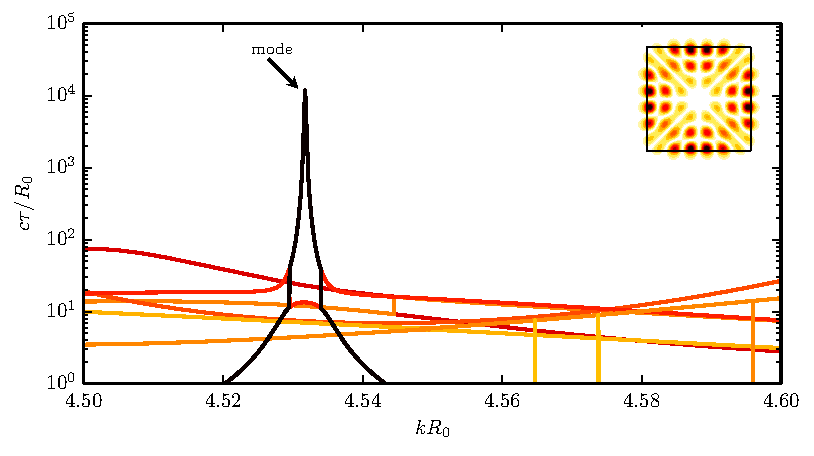
\includegraphics{figs/passive/spectrum_square_inset.pdf}
 \caption[Delay spectrum of the square cavity]
	 {Delay spectrum of the square cavity. The highlighted mode 
	 has a high $Q$-factor, which can be explained by its 
	 WGM-like field recirculation. The inset of the figure shows
	 the actual field profile of the mode. It was computed 
	 using COMSOL by G.P.-A. \cite{GAP2013a}.}
 \label{fig:passive.numerical.squareSpectrum}
\end{figure}

\section{Case Study: Gaussian Deformation of the Refractive Index}
As an academic demonstration of the power of the method, 
we present a study of a circular cavity whose refractive index
has a Gaussian shape
  \begin{equation}
   n(r,\theta) = n_0 + \delta n\exp\left[-\frac{r^2+2dr\cos\left(\Theta-\theta\right)+d^2}{2w^2}\right],
  \end{equation}
where $n_0$ is the background refractive index, $\delta _n$ the 
deformation amplitude, $w$ its half-width and $(d,\Theta)$
its position relative to the center of the cavity. 

As previously noted by G.~P-A. \cite{GAP2013a}, a peculiar
duality exists between high-$Q$ resonances and directional emission.
Working with a cavity similar to the annular one, it stands to reason
that we will recover the same pattern. This study will be used
as a stepping stone for our inquiries in the realm of non-uniformly
pumped active microcavities. 

\subsection{Loss of Integrability and the KAM Scenario}
When $d=0$, the potential is central and angular momentum is 
conserved. If the system is also unitary
(no absorption nor gain), it can be shown that the system is
integrable\footnote{The covariant form of Maxwell's equation and their
associated Euler-Lagrange equation make this conservation perfectly clear.}. 
This conservation of angular momentum in turn
implies circular symmetry of the fields and hence of the 
far-field radiation pattern. Since most applications (particularly lasers)
require a certain directionality in the emission, our goal is to break 
the circular symmetry in such a way as to minimize the degradation of the
finesse ($Q$-factor) and maximizing the output directionality. Historically, 
this goal has spawned the research field of \glspl{arc} \cite{NOC1997,HEN2002b,SCH2004a,TUR2005,HIS2013,SHU2013} wherein the boundary
of the circular cavity is parametrically deformed to yield limaçon, stadium, 
elliptical, quadrupolar, and other shapes. 

The underlying classical mechanics of \glspl{arc} follow the KAM scenario 
as the geometry is perturbed away from a perfect circle. In phase space, 
regularity yields to the chaotic sea, dividing it into regions of regular
motion and regions of ergodic motion. The Hamiltonian nature of the 
dynamics has been thoroughly studied and has been used to tame the 
animosity of directionality and high-$Q$ emission \cite{KWA2013,KIM2013}

In our case, we do not deform the boundary, leaving it a perfect circle, 
but use a deformation of the refractive index. This particular deformation
-- the Gaussian one -- 
is of theoretical and practical interest, as it can easily be induced
by shining light on the dielectric from above. This refractive
index profile is also obtained when pumping a microcavity laser
with another laser.

\subsection{Numerical Results}
Fig.~\ref{fig:passive.gaussian.numericalResults.farField} shows our primary
result, i.e. that loss of symmetry may introduce directionality
in the far-field. The directionality is mild in our example, but the 
cavity serves as a proof-of-concept. In Fig.~\ref{fig:passive.gaussian.numericalResults.spectrum}, 
the dotted blue lines show the delay spectrum of the centered Gaussian (CG) deformation, 
an integrable cavity, and the full red lines the spectrum of the non-centered Gaussian
(NG) deformation. Notice that the higher-delay modes are barely affected by 
the inhomogeneity. While we do not know the field profile, 
it is safe to assume the two high-delay modes behave like WGMs. Although it is not shown, 
both modes have isotropic far-fields. The rather small shift in wavenumber can be
understood by the slight rarefaction of the medium near the deformation. 
The field must ``evade'' being caught by the deformation to retain
its WGM properties, which results in slight positive increase in $k$ (smaller wavelength). 

\begin{figure}
 \centering
 \begin{subfigure}{0.6\textwidth}
  \centering
  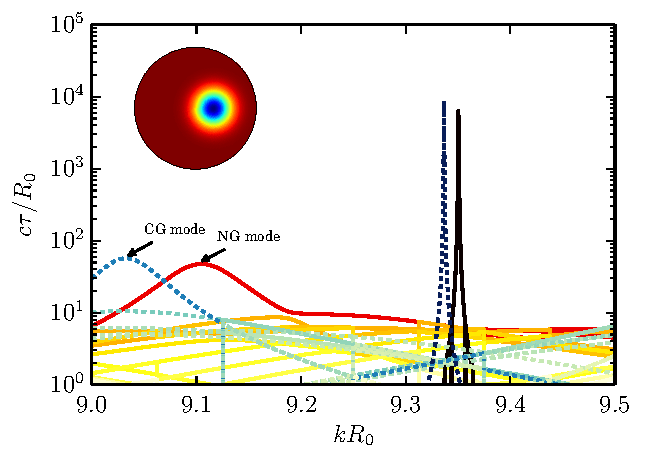
\includegraphics[width=\textwidth]{figs/passive/spectrum_gaussian_inset.pdf}
  \caption[Delay spectrum of the Gaussian microcavity]
	  {Delay spectrum of the gaussian microcavity. The dotted blue lines show the spectrum
	  for the integrable case of the deformation, i.e. $d=\Theta=0$ (CG mode). The full red lines
	  show the spectrum for the deformation centered at $d=0.3R_0$ and $\Theta=0$ (NG mode).}
  \label{fig:passive.gaussian.numericalResults.spectrum}
 \end{subfigure}
 \begin{subfigure}{0.39\textwidth}
  \centering
  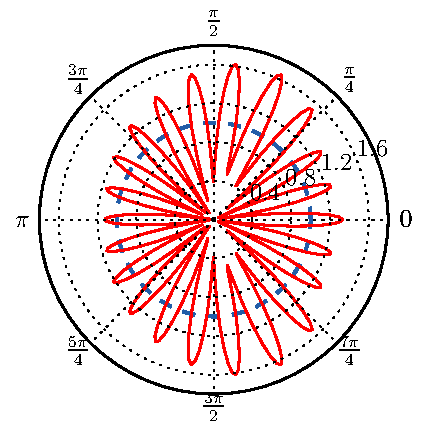
\includegraphics[width=\textwidth]{figs/passive/farField_gaussian.pdf}
  \caption{Far-fields of both CG (dotted blue) and NG (full red) modes. The isotropy is broken 
	  when the potential loses its circular symmetry. The NG mode has mild directionality
	  in the directions $\theta=\pm65^\circ$, owing to the diverging lens effect of the deformation.}
  \label{fig:passive.gaussian.numericalResults.farField}
 \end{subfigure}
 \caption[Delay spectrum of the Gaussian cavity and the far-fields of two chosen modes]
	  {Delay spectrum and far-field. \textbf{\subref{fig:passive.gaussian.numericalResults.spectrum}} 
	  Delay spectrum of cavity with the Gaussian deformation with parameters $n_0=2$, $\delta n=-1$ and $w=0.2R_0$.
	  \textbf{\subref{fig:passive.gaussian.numericalResults.farField}} shows the far-field of the both the CG and NG modes.
	  Notice the mild directionality of the NG mode.}
 \label{fig:passive.gaussian.numericalResults}
\end{figure}

The lower delay modes, the highlighted ones in \ref{fig:passive.gaussian.numericalResults.spectrum}
are more affected by the inhomogeneity, as their field must be more
extended in the dielectric. The field thus ``feels'' a greater
rarefaction of the medium and the mode suffers both a greater $\Delta k$
and a pronounced change in its emission properties. The angular momentum
mixing is such that that the ``backscattering'' $|\psi_\text{FF}(\theta=\pi)|$
is minimized and that the scattering in directions $\theta\sim\pm3\pi/8$
is favoured. This directionality may somewhat be explained by a
ray analysis of the system, as the deformation acts as a diverging
lens. The next section will explain this in more detail. 

\subsection{Geodesics and Ray Analysis\footnote{We use Schutz's \cite{SCH2009} notation in this section.
Repeated indices are summed over; $g_{\alpha\beta}$ is the metric tensor; the notation 
$M_{\alpha\beta,\gamma}$ indicates differentiation with respect to $\gamma$. The contravariant
tensor $g^{\alpha\beta}$ is the inverse of $g_{\alpha\beta}$, i.e. $g^{\alpha\beta}g_{\beta\gamma}={\delta^\alpha}_\gamma$.}}
While our numerical method allows us tu perform full-wave
simulations of cavities, it is often useful to consider the associated
billiard\index{billiard} system, which is the small wavelength approximation of 
Helmholtz's equation. In homogeneous ARCs\index{asymmetric resonant cavity}, photons follow straight path
trajectories and are specularly reflected at the interfaces. In inhomogeneous
\glspl{arc}, photons follow curved trajectories that obey Fermat's principle. 
The general equations defining those \textit{geodesic} paths can be found
by using the metric
  \begin{equation}
   (dt)^2=g_{\mu\nu}dx^\mu dx^\nu. 
  \end{equation}
For photons, the metric is simply given by the optical length 
of the medium, $g_{\mu\nu}=n^2(\bo{r})\delta_{\mu\nu}$. 
The time it takes to travel a particular trajectory is given by
  \begin{equation}
   t = \int_{\lambda_0}^{\lambda_1} \sqrt{g_{\mu\nu}\dot{x}^\mu\dot{x}^\nu}\,d\lambda
  \end{equation}
where $\lambda$ is a parameter of the curve. By Fermat's principle, photon 
trajectories minimize the time of flight. We thus apply the Euler-Lagrange
equation 
  \begin{align}
   \frac{\partial L}{\partial x^\alpha}-\frac{d}{d\lambda}\frac{\partial L}{\partial\dot{x}^\alpha}=0
  \end{align}
on the functional $L=\sqrt{w}=\sqrt{g_{\mu\nu}\dot{x}^\mu\dot{x}^\nu}\,d\lambda$ Evaluating the derivatives
  \begin{align*}
  0	&=\frac{\partial\left(\sqrt{w}\right)}{\partial x^\alpha}-\frac{d}{d\lambda}\frac{\partial\left(\sqrt{w}\right)}{\partial\dot{x}^\alpha}	\\
  {}	&=\frac{\partial w}{\partial x^\alpha}+\frac{1}{2\sqrt{w}}\frac{dw}{d\lambda}\frac{\partial w}{\partial\dot{x}^\alpha}-\frac{d}{d\lambda}\frac{\partial w}{\partial\dot{x}^\alpha}
  \end{align*}
When $\lambda$ is an affine parameter, the derivative $dw/d\lambda$ vanishes \cite{TOP2005,SCH2009}
and the Euler-Lagrange equation becomes
  \begin{align*}
  \frac{\partial w}{\partial x^\alpha}			&= \frac{d}{d\lambda}\frac{\partial w}{\partial\dot{x}^\alpha}	\\
  g_{\mu\nu,\alpha}\dot{x}^\mu\dot{x}^\nu		&= \frac{d}{d\lambda}\left[g_{\mu\nu}{\delta_\alpha}^\mu\dot{x}^\nu+g_{\mu\nu}{\delta_\alpha}^\nu\dot{x}^\mu\right]	\\
							&= \frac{d}{d\lambda}\left[g_{\alpha\nu}\dot{x}^\nu+g_{\mu\alpha}\dot{x}^\mu\right]					\\
							&= g_{\alpha\nu,\lambda}\dot{x}^\lambda\dot{x}^\nu+g_{\alpha\nu}\ddot{x}^\nu+g_{\mu\alpha,\lambda}\dot{x}^\lambda\dot{x}^\mu+g_{\mu\alpha}\ddot{x}^\mu \tag{chain rule: $\frac{dg_{\mu\nu}}{d\lambda}=\frac{\partial g_{\mu\nu}}{\partial x^\lambda}\frac{dx^\lambda}{d\lambda}$}	\\
  g_{\alpha\nu}\ddot{x}^\nu+g_{\mu\alpha}\ddot{x}^\mu	&= \dot{x}^\mu\dot{x}^\nu\left[g_{\mu\nu,\alpha}-g_{\alpha\nu,\mu}-g_{\mu\alpha,\nu}\right]	\tag{collecting differentiation orders}	\\
  {\delta^\sigma}_\mu\ddot{x}^\mu			&= \frac{1}{2}g^{\sigma\alpha}\left[g_{\mu\nu,\alpha}-g_{\alpha\nu,\mu}-g_{\alpha\mu,\nu}\right]\dot{x}^\mu\dot{x}^\nu	\tag{symmetry of $g_{\mu\nu}$ and $\times g^{\sigma\alpha}$}
  \end{align*}
This finally yields the equation
  \begin{equation}
   \ddot{x}^\sigma + {\Gamma^\sigma}_{\mu\nu}\dot{x}^\mu\dot{x}^\nu=0
  \end{equation}
where ${\Gamma^\sigma}_{\mu\nu}$ are the Christoffel symbols of the second kind. 

This last equation describes the trajectories of classical photons in any media. 
At interfaces, where the optical parameters have a jump discontinuity, one must use
Fresnel's laws, and possibly their generalization for curved interfaces \cite{HEN2002a}.

We will now obtain the equations for our Gaussian deformation. The author of this essay
would have expected that an analytical solution be available for the central Gaussian
potential, but the non-linearity of the equations spoil the symmetry and the hopes 
of finding a solution. We will thus solve the equations in Cartesian coordinates
for the centered formation:
  \begin{equation}
   n(x,y) = n_0 + \delta n \exp\left[-\frac{x^2+y^2}{2w^2}\right].
  \end{equation}
In Cartesian coordinates, the six independent Christoffel symbols have
value
  \begin{align*}
   {\Gamma^x}_{xx}			&= \frac{n_x}{n}	&	{\Gamma^y}_{xx}	&=-\frac{n_y}{n}\\
   {\Gamma^x}_{xy}={\Gamma^x}_{yx} 	&= \frac{n_y}{n}	&	{\Gamma^y}_{xy}={\Gamma^y}_{yx}&=\frac{n_x}{n}\\
   {\Gamma^x}_{yy}			&= -\frac{n_x}{n}	&	{\Gamma^y}_{yy}	&=\frac{n_y}{n}
  \end{align*}
which yield the equations
  \begin{subequations}
  \begin{align}
   \ddot{x}	&= \frac{x/w^2}{1+\frac{n_0}{\delta n}\exp\left[\frac{x^2+y^2}{2w^2}\right]}\left(\dot{x}^2-\dot{y}^2\right)
	    +\frac{2y/w^2}{1+\frac{n_0}{\delta n}\exp\left[\frac{x^2+y^2}{2w^2}\right]}\dot{x}\dot{y}				\\
   \ddot{y}	&= \frac{y/w^2}{1+\frac{n_0}{\delta n}\exp\left[\frac{x^2+y^2}{2w^2}\right]}\left(\dot{y}^2-\dot{x}^2\right)
		  +\frac{2x/w^2}{1+\frac{n_0}{\delta n}\exp\left[\frac{x^2+y^2}{2w^2}\right]}\dot{x}\dot{y}.
  \end{align}
  \end{subequations}
We seperate the two second-order equations in four first-order equations by defining $p_x=\dot{x}$ and $p_y=\dot{y}$. 
We solve the equations for photons coming in from $x(0)\rightarrow-\infty$ with $p_x(0)=\text{const}$
and $p_y(0)=0$ for different values of the impact parameters $y(0)=b$. The results are shown in 
Fig.~\ref{fig:passive.gaussian.geodesics} and from this simple analysis we see that 
the deformation acts as a diverging lens. 
\begin{figure}
 \centering
 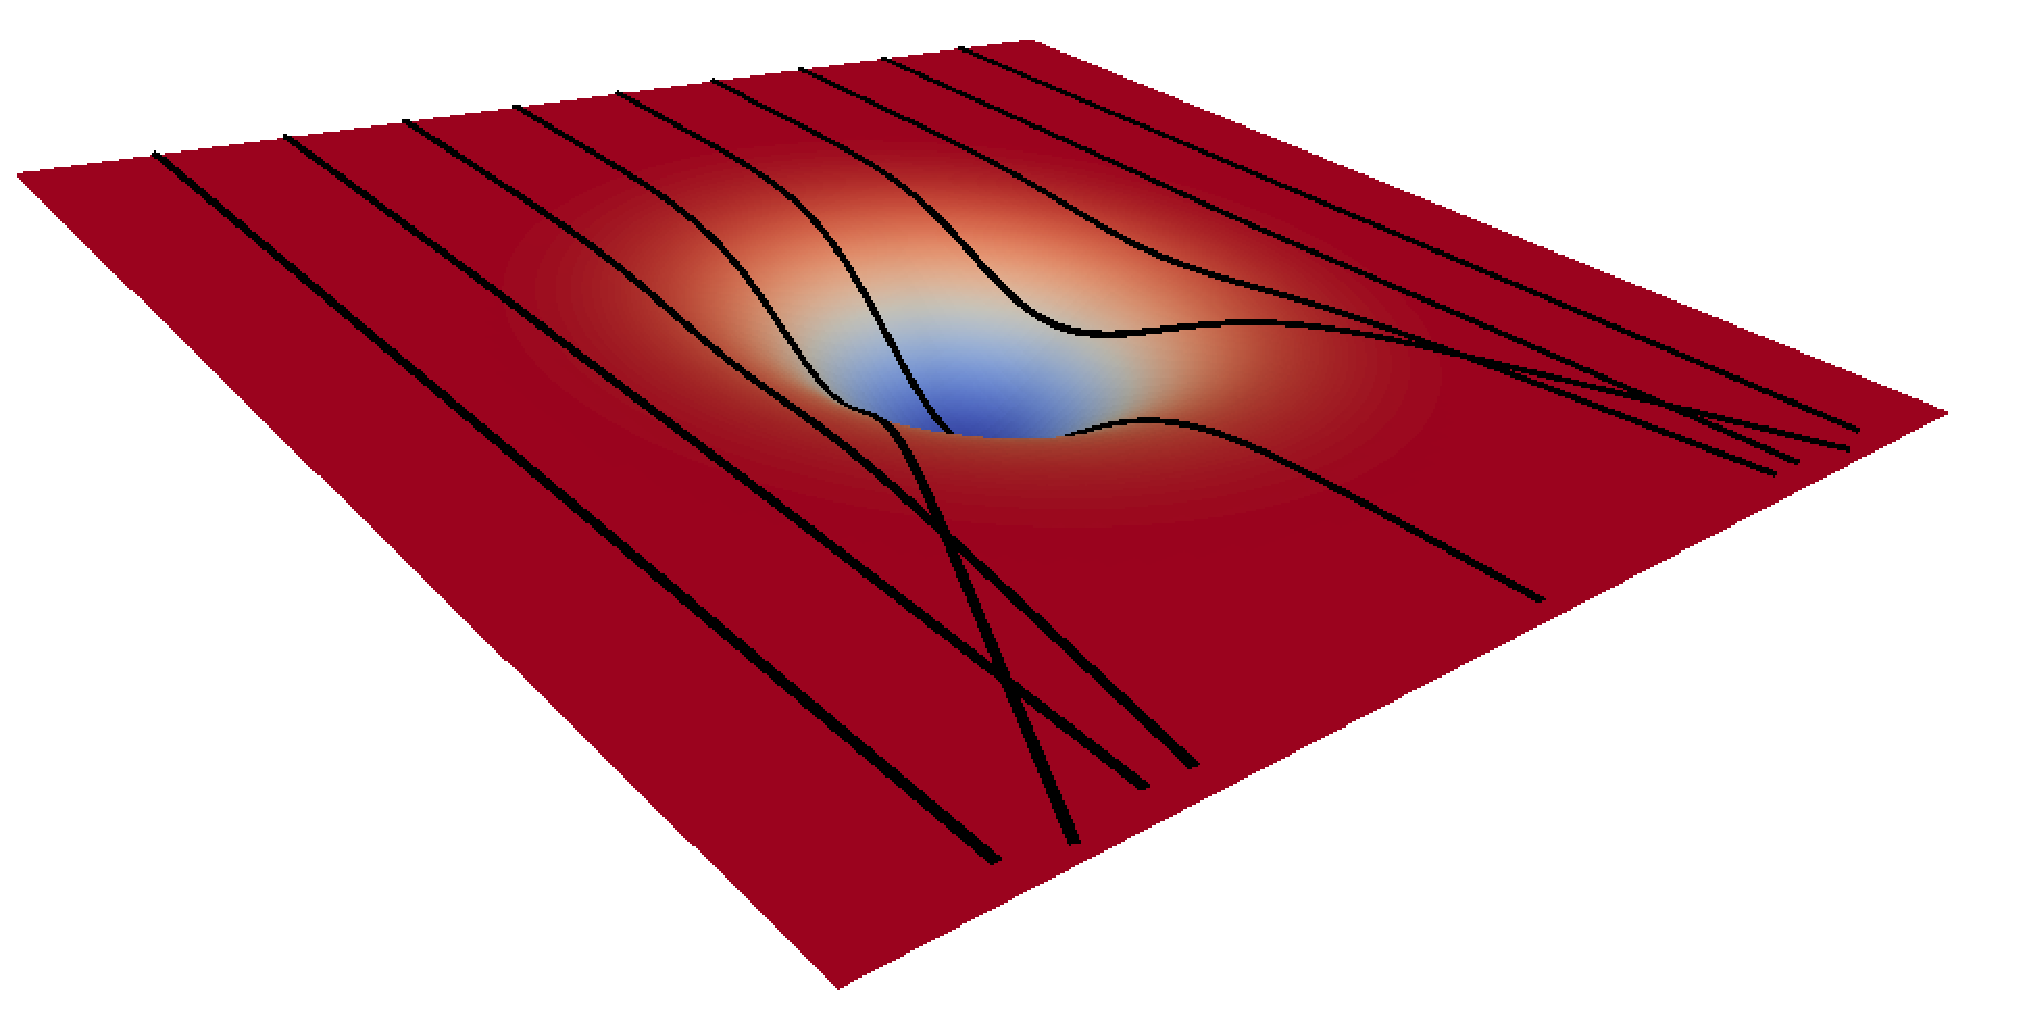
\includegraphics[width=0.75\textwidth]{figs/passive/geodesics-1.eps}
 \caption[Photon trajectories in a Gaussian deformation of the refractive index]
	  {Trajectories for photons of different impact parameters. The trajectories are
	  the geodesics of the relevant ``optical spacetime'', where the curvature of 
	  space represents the optical distance that the photon has to traverse. The central
	  region, where the refractive index is lower, acts as a diverging lens.}
 \label{fig:passive.gaussian.geodesics}
\end{figure}

From these equations, a more sophisticated algorithm could be developed to study
the associated classical mechanics of inhomogeneous billiard systems, as was done
in \cite{SAI2005}. The algorithm would need to include collision detection with the 
boundary of the billiard as well as formulas for the reflection and transmission coefficients
at this boundary.

\section{Conclusion and Perspectives}
This section solved the scattering problem of bidimensional
dielectric cavities\index{dielectric resonators}. Using information on the real $k$-line,
the \gls{qMatrix} allows for the computation of the complex poles
of the scattering matrix, which in turn correspond to the resonances
of the scatterer. The eigenvectors of the \gls{qMatrix} define 
a set of modes that exist each real value of $k$. The eigenvectors
which correspond to peaks in the time delay spectrum can be associated
with the complex poles of $\mat{S}(k)$.

The formalism is coupled to a numerical method that computes 
the scattering matrix for inhomogeneous bidimensional cavities.
The method is based on an onion-like discretization scheme
where the solution of Helmholtz's equation can be reduced to an 
eigenvalue problem. This leads to the construction of local, or 
``shell scattering matrices''. The boundary conditions allow to fuse
the shells of the onion and compute the effect of the whole scatterer, 
viz. the scattering matrix.

The method is fast enough that it is possible to consider
an optimization problem with one or several cost functions
that quantify the performance of the scatterer for a
given application. A few examples spring to mind, such as
a dielectric optical switch, beam splitters, biosensors and others. 
If the material is active, one cold optimize the form of the pump 
profile to minimize thresholds and maximizing, for instance, output
directionality and power. This will be discussed in the following chapter.

One subject we have failed to mention in the main text is the 
fragility of the generalization of the \gls{sqa} to complex
energies $k$ and potentials $n$; it also becomes computationally
heavy. The details of the fragility are discussed in Appendix
\ref{sec:app.numTools.scatMat}. This, coupled to the instabilities
related to the reconstruction of the field inside the scatterer
has been a motivation to look for other numerical methods. In 
the next chapter, we will develop an \textit{integral} method
for the computation of the scattering matrix. This flexible
method will be use of great use in discussing active material 
and 3D geometries. 

% %From the general to the specific, scattering methods to solve
% %Maxwell's equations. 
% 
% \begin{itemize}
%  \item Lippmann-Schwinger type method. 
%   \begin{itemize}
%     \item Allows for full control over discretization. 
%     \item Takes Sommerfeld radiation condition into account analytically.
%     \item Must perform solution of vectorial 3D Fredholm equation. 
%   \end{itemize}
%  \item SQA
%   \begin{itemize}
%     \item Derivation of equations.
%       \begin{itemize}
% 	\item Effective Index Approximation and $\beta=0$.
% 	\item TM + TE polarizations.
%       \end{itemize}
%     \item Generalization of method to complex $n$.
%       \begin{itemize}
% 	\item Dual basis. 
% 	\item Numerical analysis of algorithm.
%       \end{itemize}
%     \item Difficulty: Field reconstruction. 
%   \end{itemize}
%  \item Variable Phase Method
%   \begin{itemize}
%     \item Derivation for 2D (3D?)
%     \item Results
%   \end{itemize}
%   
% \end{itemize}

% !TeX root = ../msc_thesis_jayd.tex
\chapter{Active Media and Radiation}
The previous chapter set the stage for the study of 
the scattering of light on general, albeit passive, 
potentials. The relative simplicity of the geometry
and of the physics allowed for a solution rich 
in physical information and lead to a rather simple
numerical solution. 

In the first section, we test the limits of the our analytical formalism
and of our numerical advances. To more accurately model
microlasers, we model the interaction of light with the underlying
quantum gain medium, i.e. we solve the Maxwell-Bloch, or Schrödinger-Bloch, 
matter equations. We will specifically use the \gls{salt}, a recently 
formulated steady state laser theory. In this theory, the effect 
of the active medium is reduced to an additional frequency and pump-dependent
term in the refractive index. This extra term has a Lorentzian frequency
dependence, as physically expected, and has non-zero real and imaginary
parts. The fragility of our extension of SQA is then exposed and some replacement
methods are suggested. 

The second section studies the experimental response
of different realizations of a specific type of antenna
known as \glspl{lcx}. The genesis of this study lies in
the hopes of designing an antenna that can be seamlessly
integrated into textile. The sheer complexity of the
antenna, as we will show, bars the use of the methods developed
in this essay in favour of the all-numerical \gls{fem}. 
This particular choice will be motivated and the design 
parameters of the antenna thoroughly explained. 

\section{Lasing and Scattering}
A recently formulated laser theory, named the 
\gls{salt} and developed by A. D. Stone's group
at Yale, has been shown to be an accurate model 
of the light-matter interaction involved in bidimensional
microlasers. Its steady-state nature allows us to apply
the formalism developed in the previous section 
to the theory. However, in light of the several shortcomings
of the \gls{sqa}'s numerical implementation, we have studied 
two other numerical methods. The first one, the \gls{vpm}, is based on 
differential equations and shares some of the problems of 
the onion method, but has a nice physical interpretation
in terms of phases and is more easily generalizable to 
3D scattering. 
To find a more robust solution, we completely forgo 
differential equations in favour of integral ones. 
Our brief incursion into the rich field of integral equations
is a rather recent one, and might leave the reader hungry for more.

\subsection{Primer on Steady State ab initio Laser Theory (SALT)}
Our exposition of \gls{salt} will be divided into two main sections:
the first will describe the details of the interaction of light with
the quantum gain medium and provide a steady-state solution
of the resulting Maxwell-Bloch equations. The second
will discuss the constant-flux states and their computation
using the aforementioned numerical methods. 

\paragraph{Solving the Matter Equations}
Our starting point, as always, is
  \begin{align}
   \nabla\times\bo{E}	&= ik\mu\bo{H};	&	\nabla\times\bo{H}	&= -ik\epsilon\bo{E}-ik\bo{P}^{NL}
  \end{align}
where $\bo{P}^{NL}$ now represents the possibly non-linear response
of the underlying quantum gain medium to the electric field $\bo{E}$.
We separate the fields in transverse and longitudinal
components, as we did for the passive cavities. Assuming 
that the propagation constant $\beta$ vanishes, we can 
separate two polarization states and write decoupled differential
equations for the longitudinal components of the fields
	\begin{subequations}
	\begin{align}
		\left[\nabla^2+k^2n^2\right]E_z	&= \frac{1}{\mu}\nabla E_z\cdot\nabla\mu -k^2\mu P_z	\tag{\theequation.TM}\\
		\left[\nabla^2+k^2n^2\right]H_z	&= \frac{1}{\epsilon}\nabla H_z\cdot\nabla\epsilon-
											\frac{ik}{\epsilon}\bo{P}^{NL}\times\nabla\epsilon
											-ik\nabla\times\bo{P}^{NL}							\tag{\theequation.TE}\label{eq:active.salt.TEeqn}
	\end{align}
	\end{subequations}
where the last equation is the \textit{proper} generalization for TE modes. 
To derive these equations, we made the implicit assumptions that the 
non-linear electric susceptibility tensor, 
	\begin{equation}
		\bo{P}^{NL} = \bo{\chi_e}^{NL}(\bo{r};\omega)\bo{E}(\bo{r}),
	\end{equation}
is at least a diagonal tensor, or a scalar. In the TM polarization, 
$E_r=E_\theta=0\Rightarrow P_r=P_\theta=0$, such that $\bo{P}^{NL}$
has a single non-zero component, while in the TE polarization only
the $P_r$ and $P_\theta$ components are non-zero. The vectors resulting
from the cross-product and curl in \eqref{eq:active.salt.TEeqn} possess
only a $z$-component, as needed. 

To go any further, we must compute the value of the non-linear electric
susceptibility tensor. 
To show the main features of the theory, we assume a two-level quantum 
system as the gain medium, although the method is generalizable to 
multi-level systems \cite[\S2.3]{GE2010b}. 

\begin{figure}
 \begin{center}
 \begin{tikzpicture}[scale=1.5]
  % -- Draw quantum system. 
  \draw[very thick] (0,0) -- (2,0) node[right] {$\Ket{1}$};
  \draw[very thick] (0,2) -- (2,2) node[right] {$\Ket{2}$};
  \draw[thick,->,>=stealth] (1,2) -- (1,0) node[near end,right] {$\gamma_\parallel$};
  
  % -- Draw incoming light.
  \draw[decorate,decoration={snake,amplitude=0.5cm,segment length=0.5cm}] (-3,1) -- (-0.25,1);
  \draw[->,>=stealth] (-2.5,1.8) -- (-.75,1.8) node[midway,above] {$\bo{E}$};
 \end{tikzpicture}
 \end{center}
 \caption[Pictorial representation of the quantum gain medium]
	 {Pictorial representation of the interaction between the
	 quantum gain medium and the incoming field. The quantum system has 
	 two levels, the wavefunction being either $\Ket{1}$ or $\Ket{2}$. The relaxation
	 rate from level 2 to level 1 is given by $1/\Gamma_{21}$.}
 \label{fig:active.salt.twoLevelSystem}
\end{figure}

Solving Schrödinger's equation for a ``bare'', i.e. non-interacting
two-level system yields
  \begin{equation}
   H_0\Ket{\psi}=\omega_j\Ket{\psi}	\qquad j=0,1
  \end{equation}
and corresponding eigenfunctions $\Ket{1}$ and $\Ket{2}$. 
The incoming light field acts as a perturbation and source of energy
that stimulates a population transfer from level 1 to level 2 that decay
at rate $1/\gamma_\parallel$. The perturbation can be written as
  \begin{equation}
   H_1 = e\bo{\mu}\cdot\bo{E}
  \end{equation}
where $e$ is the electric charge and $\bo{\mu}$ is the 
dipole moment tensor of the material.  We expand the solution 
of the perturbed in the states of the unperturbed system
  \begin{equation}
   \Ket{\psi_1(t)}=C_1(t)\Ket{1}+C_2(t)\Ket{2}
  \end{equation}
and form the density matrix
  \begin{equation}
   \rho(t) = \Ket{\psi_1(t)}\Bra{\psi_1(t)}.
  \end{equation}
It allows us to solve the problem for an ensemble
of two-level systems \cite{GE2010b}.
Using the well-known evolution equations of the density
matrix \cite[\S6.2]{BOY2008} and defining
$D=\rho_{22}-\rho_{11}$, the population difference between the two
levels,  we obtain the equations
\cite[\S5.3]{HAK1985b}
  \begin{align}
   \dot{\bo{P}}^{NL}	&= -\left(i\omega+\gamma_\perp\right)\bo{P}^{NL}+\frac{g^2}{i\hbar}\bo{E}D	\\
   \dot{D}				&= \gamma_\parallel\left(D_0-D\right)-\frac{2}{i\hbar}\bo{E}\cdot\bo{P}^{NL}
  \end{align}
where $g^2$ is the dipole moment of the system, 
$\gamma_\perp$ is an \textit{ad hoc} phenomenological damping
term that comes from the interaction of the ensemble of two-level systems\footnote{The author surmises that it 
could be computed with a mean field approximation.}
and $D_0$ is the equilibrium population. The approach 
uses a \gls{rwa}, but, contrary 
to most derivations, does not invoke the \gls{svea}. 
One of the main approximations, one that is necessary to make
ground, is the \gls{sia}, i.e. $\dot{D}=0$. Writing the fields
as Fourier series
	\begin{align*}
		\bo{P}^{NL}	&= \sum_{\mu}\bo{p}_\mu e^{-ik_\mu t}	&	\bo{E}	&= \sum_{\mu} \bo{\Psi}_\mu e^{-ik_\mu t}
	\end{align*}
leads to the relationship\footnote{We have skipped some steps. See \cite[\S2.2]{GE2010b} for details.}
  \begin{equation}
   \bo{p}_\mu = \frac{g^2}{\hbar}\frac{1}{k_\mu-k+i\gamma_\perp}\frac{D(\bo{r})}{1+\sum\frac{4g^2}{\gamma_\perp\gamma_\parallel}\Gamma(k_\mu)\left|\Psi_\mu(\bo{r})\right|^2}\bo{\Psi}_\mu(\bo{r}).
  \end{equation}
In the TM polarization, this leads to the equation
  \begin{equation}
   \left[\nabla^2+k^2\left(\epsilon(\bo{r})+\frac{g^2}{\hbar}\frac{1}{k_\mu-k+i\gamma_\perp}\frac{D(\bo{r})}{1+\sum_\mu\frac{4g^2}{\gamma_\perp\gamma_\parallel\Gamma(k_\mu)}\left|\Psi_\mu(\bo{r})\right|^2}\right)\right]\Psi_\mu(\bo{r})=0
  \end{equation}
where
	\begin{equation}
		\Gamma(k_\mu) = \frac{\gamma_\perp^2}{(k-k_\mu)^2-\gamma_\perp^2}
	\end{equation}
$\Psi_\mu(\bo{r})$ is the longitudinal component of the field. 

\paragraph{Constant-flux States and Scattering}
The derivation above, novel to SALT and slightly more accurate
than the standard derivations \cite{GE2010a,GE2010b,EST2013}, shows
that the effect of the quantum gain medium can be modeled as an extra
term in the refractive index in the TM polarization, but leads to an altogether
different differential equation in the TE polarization. To the author's knowledge,
this is never specifically addressed in the SALT articles, except in the vectorial
generalization of SALT \cite{GE2010b}. In the following, we will also focus on the
TM polarization. 

The central feature of \gls{salt} is the introduction of the constant-flux (CF)
states, which are defined by
	\begin{subequations}
	\begin{align}
		\left[\nabla^2+\epsilon(\bo{r})K^2(k)\right]\psi(\bo{r})	&=	0	& \bo{r}\in\mathcal{C}		\label{eq:active.salt.cfCavity}\\
		\left[\nabla^2+\epsilon(\bo{r})k^2\right]\psi(\bo{r})		&=	0	& \bo{r}\notin\mathcal{C}	\label{eq:active.salt.cfOutside}
	\end{align}
	\end{subequations}
where $\mathcal{C}$ is the cavity region. Inside $\mathcal{C}$, 
the frequency $K(k)$ is allowed to be complex, but outside the cavity
we force $k$ to be real. This allows us to bestow physical meaning
unto the CF states, as they do not suffer from the exponential
growth of the QB states. Despite the non-linearity of the equations, 
the CF states can be used as a basis for the laser modes, and can even 
take into account saturation, spatial hole burning and non-uniform
pumps through the 
	\begin{equation*}
		\label{eq:active.salt.tlms}
		\frac{D(\bo{r})}{1+\sum_\mu\frac{4g^2}{\gamma_\perp\gamma_\parallel}\left|\Psi_\mu\right|^2}
	\end{equation*}
term. If we restrict our analysis to near-threshold modes, we can neglect the sum in the previous term
and, writing the pump profile as a pump strength multiplied by a shape function $D(\bo{r})=D_0F(\bo{r})$, 
we obtain
	\begin{align}
		\left[\nabla^2+k^2\left(\epsilon(\bo{r})+\frac{\gamma_\perp D_0F(\bo{r})}{k_\mu-k+i\gamma_\perp}\right)\right]\psi &=0 & \bo{r}\in\mathcal{C}
	\end{align}
where now the fields and the pump strength are dimensionless parameters measured in units of $D_{0c}=\hbar\gamma_\perp/(4\pi g^2)$
and $e_c = \hbar\sqrt{\gamma_\parallel\gamma_\perp}/(2g)$, respectively \cite[p.~19--20]{GE2010b}. 
The solutions of this equation describe the lasing action near lasing thresholds, the threshold lasing modes (TLMs). 
In the case of uniform pumping, i.e. $F(\bo{r})=1$,
CF are in a one-to-one correspondence with TLMs, as we can see by comparing
\eqref{eq:active.salt.cfCavity} and \eqref{eq:active.salt.tlms}. To find
the TLMs, one needs to compute the CF states and find the values of $K^2(k)$
infer the values of $D_0$. When the exterior frequency $k$ is such that $D_0$
is real, the resulting couple $(k_a, D_0^a)$ reveals the frequency and threshold
of the lasing mode. This was done in \cite{GAG2014a}. 

However, we will mostly be interested in the case of non-uniform pumping
and/or inhomogeneous refractive index distribution. To find the couple
$(k_a,D_0^a)$, we must solve \eqref{eq:active.salt.tlms} self-consistently
for a real value of $D_0$ such that a pole of scattering matrix hits 
the real $k$-line. In the following sections, we will propose two
numerical methods that can compute the non-unitary scattering matrix
of our problem and determine its poles. Our last method can also 
treat the spatial hole burning term and compute the non-linear 
\gls{sMatrix}.

\subsection{Methods of Solution}
\paragraph{Variable Phase Method}
This elegant method has its roots deep in the literature of quantum-mechanical
scattering. It is based on the fact that, for central potentials, the 
\gls{sMatrix} is diagonal and that its elements can be written as
$e^{i\delta_k}$, where $\delta_k$ is the phase shift suffered by the 
$k$th partial wave. One can thus find a first order, non-linear differential
equation \cite{CAL1967} for each $\delta_k$. The method transforms the \gls{bcp} to an \gls{ivp}, as the phase shift
is bounded. In our present case, the potential is not a central one and the
\gls{sMatrix} is not diagonal. We will need to solve a coupled system 
of differential equations to represent the coupling between the different
partial waves. The \gls{vpm} will give rise to an \gls{ivp} matrix \gls{ode}.

The initial motivation for the use of \gls{vpm} was the computation 
of the field inside the scatterer. In the \gls{sqa}, modifying 
the linear algebra operations of the reduction phase yields
an algorithm that computes the field from given $\bo{A}$ and $\bo{B}$
coefficients. It is unfortunately highly unstable, to the point 
of being unusable. The authors of \cite{FOR2012} suggested that
the \gls{vpm} was stable, suggesting its use over the onion
discretization of \gls{sqa}. While the \gls{vpm} has some inherent
issues and our implementation is far from complete, we present
here the main development both for the interested reader and for 
future reference. 

The method starts with the angular momentum expansions
  \begin{subequations}
  \begin{align}
   H_z(r,\theta)	&= \frac{1}{\sqrt{2\pi}}\sum_{m=-\infty}^\infty \frac{1}{\sqrt{r}}\psi_m(r)e^{im\theta}	\\
   n(r,\theta)		&= \frac{1}{\sqrt{2\pi}}\sum_{m'=-\infty}^\infty n_{m'}(r)e^{im'\theta}.
  \end{align}
  \end{subequations}
Substituting these expansions in Helmholtz's equation and projecting
onto the eigenstate 
	\begin{equation*}
		\sqrt{r}e^{-im''\theta}/\sqrt{2\pi}
	\end{equation*} 
yields a system of coupled \glspl{ode} for each moment of the field $\psi_m$
	\begin{equation}
		\label{eq:active.vpm.equation}
		\bo{\psi}''-\frac{\mat{M}^2-\mat{I}/4}{r^2}\bo{\psi}+\frac{k^2}{2\pi}\mat{N}^2\bo{\psi}=0
	\end{equation}
where 
	\begin{equation*}
		\left[\mat{N}(r)\right]_{mm''}=\sum_{m'}n_{m'}(r)\delta_{m+m',m''}.
	\end{equation*}
Notice that the free case is recovered when $n(r,\theta)=1$, as 
then $n_{m'}=\delta_{m'0}$ and 
	\begin{equation}
		\bo{\psi}''-\frac{\mat{M^2}-\mat{I}/4}{r^2}\bo{\psi}+k^2\bo{\psi}=0
	\end{equation}
a system of uncoupled Bessel equations. At this point, we 
introduce the matrix \gls{ode}, i.e. \eqref{eq:active.vpm.equation} with as many 
rows as columns. Each column solves the ODE, but has different boundary conditions
\cite[\S15.2]{NEW1982}. Since the scattering solution must obey Sommerfeld's radiation
condition, we use the factorization
	\begin{equation}
		\bo{\psi} = \mat{G}_k(r)\mat{W}^{+}(kr)
	\end{equation}
where $\left[\mat{W}^{\omega}(kr)\right]_{mm''}=H_m^{(\omega)}(kr)\delta_{mm''}$.
Outside the \gls{lss}, the solution must be $\mat{W}^+(kr)$. In the general potential
scattering theory, the \gls{lss} is usually a sphere at infinity, which yields the 
initial value conditions
	\begin{align}
		\mat{G}_k(\infty)	&=\mat{I}	&	\mat{G}_k'(\infty)=\mat{0}.
	\end{align}
with 
	\begin{equation}
		\mat{G}_k''+2\mat{G}_k'\frac{d\log\mat{W}^\omega}{dr}+\frac{1}{r^2}\left[\mat{G}_k,\mat{M}^2-\mat{I}/4\right]
					+\frac{k^2}{2\pi}\left(\mat{N}^2-2\pi\mat{I}\right)=0.
	\end{equation}

The $\mat{G}_k(r)$ matrix represents the phase shifts accumulated by each partial wave $m$ 
and caused by the $m'$th angular moment of the potential. The factorization procedure 
effectively transforms the \gls{bcp} to an \gls{ivp}, with the data provided on the 
\gls{lss}. The matrix ODE can thus be solved by using any good integration routine\footnote{Although
make sure you use a stiff equation solver. See Appendix \ref{sec:app.numTools.vpm} for details.}.

The scattering matrix of the problem can also be obtained if we 
compute the conjugate solution, solving with the incoming radiation $\bo{\psi}=\mat{G}_{-k}\mat{W}^-(kr)$
instead of the outgoing one. The physical wave function is thus given by 
	\begin{equation}
		\bo{\psi} = \mat{G}_{-k}(r)\mat{W}^-(kr)+\mat{G}_k(r)\mat{W}^+(kr)\mat{S}_k(k).
	\end{equation}
Using the finiteness condition of the field at origin, we have
	\begin{equation}
		\mat{S}_k = -\lim_{r\rightarrow0}\mat{W}^{+}(kr)^{-1}\mat{G}_k^{-1}(r)\mat{G}_{-k}(r)\mat{W}^-(kr).
	\end{equation}

\paragraph{Green's Function Method}
Seeing the differential methods fail, the author of this essay, 
then on the brink of despair, first took notice of the 
power of integral methods. Simply rewriting Helmholtz's 
equation as
  \begin{equation}
   \left[\nabla^2+\epsilon_B(\omega)k^2\right]\psi=-k^2\Delta\epsilon(\bo{r};\omega)\psi
  \end{equation}
where 
  \begin{equation}
  \Delta\epsilon(\bo{r};\omega)=\epsilon(\bo{r};\omega)-\epsilon_B(\omega)
  \end{equation}
where $\epsilon(\bo{r};\omega)$ is the permittivity profile of the scatterer
and $\epsilon_B(\omega)$ the constant permittivity of the environment, or background.
This allows to write a formal solution using the Green's function of Helmholtz's equation
  \begin{equation}
  	\label{eq:active.vpm.fredholmEqn}
  	\psi(\bo{r}) = \phi(\bo{r}) - k^2\mathop{\iint}_\mathcal{C}G_{+}(\bo{r},\bo{r}')\Delta\epsilon(\bo{r}';\omega)\psi(\bo{r}')d^2\bo{r}'
  \end{equation}
where $\phi(\bo{r})$ is a solution of the homogeneous problem and
  \begin{equation}
  	G_\omega(\bo{r},\bo{r}') = -\frac{i}{4}H_0^{(\omega)}(k\sqrt{\epsilon_B}|\bo{r}-\bo{r}'|).
  \end{equation}
While \eqref{eq:active.vpm.fredholmEqn} is very general: it can be applied to 
any $\Delta\epsilon(\bo{r};\omega)$, even to non-linear problems, 
the method of solution we will use restricts us to linear problems.

Instead of a \gls{pde}, we now must solve an implicit 
integral equation for the field. It is a Fredholm 
equation of the second kind with a weakly singular, compact
operator. This ensures the existence
and uniticity of the solution \cite{GOH1981,COL2013}.
We solve the surface integral equation in real space by meshing
the cavity $\mathcal{C}$. The details of the meshing is left to 
Appendix \ref{sec:app.basisEqn.greenFunction}. Let us denote the set
of cells of our mesh by $\Delta$. We can thus cast the integral
equation as
	\begin{equation}
		\psi_j = \phi_j -k^2\sum_{j'\in\Delta} G_{jj'}\Delta\epsilon_{j'}A_{j'}\psi_{j'}
	\end{equation}
where $\psi_j=\psi(\bo{r}_j)$ and similarly for the other quantities. We can
rewrite this as the matrix problem\footnote{This, of course, only holds if the
kernel is linear.} 
	\begin{equation}
		\left(\mat{I}+\mat{K}\right)\bo{\psi}=\bo{\phi}.
	\end{equation}
where 
	\begin{equation}
		K_{jj'} = G_{jj'}\Delta\epsilon_{j'}A_{j'}.
	\end{equation}

The matrix equation is then solved using any good 
linear algebra solver. This yields values for the
field inside the scatterer. The integral equation
is then explicit for the field outside the scatterer. 
Our interest, however, still lies in the computation
of the scattering matrix. It turns out that, if we
use 
	\begin{equation}
		\phi = J_M(kr)e^{iM\theta}
	\end{equation}
as the ``incoming'' field, one may find that the scattering
matrix can be computed via
	\begin{equation}
		S_{mM} = \delta_{mM} - \frac{ik^2}{2}\mathop{\iint}_\mathcal{C}e^{-im{\theta'}}J_m(kr')\Delta\epsilon(\bo{r}')\psi^{(M)}(\bo{r}')d^2\bo{r}'.
	\end{equation}
In Appendix \ref{sec:app.basisEqn.greenFunction}, we lay out the method in more detail, 
discuss the numerical implementation and present a generalization for the complete 
vectorial electromagnetic fields.

\subsection{Examples}

\section{Smart Textile Antennae}
The last part of this essay recounts the author's contributions
in a project involving the design and theoretical characterization
of fibre-antennas. This section departs a little from the more theoretical
and numerical musings of the others and presents both the modeling of the 
antennae and their experimental characterization.   

The goal of the original project was to develop an antenna that is compatible with 
WiFi standards (i.e. emits at $f=2.45\,\unit{GHz}$) and can be easily integrated
to textile. These two requirements impose multiple restrictions on both
the materials that can be used and the geometry of the antenna. For instance, 
we would like the antenna to be spun directly into the textile as to have, 
so to speak, a seamless integration of the antenna.

Most solutions today merely affix a patch antenna to a less 
encumbered part of the textile \cite{CAT2004,JAI2013}, e.g. 
on the should pads of a shirt or the front of a t-shirt.
A metallic plate shields the user from the electronic components 
of the patch antenna. Because the properties of patch antennas are
well known \cite{ELL2003}, very little engineering is required and this solution
is thus quite cheap\footnote{The general availability of consumer-grade ``smart''
textile on the Web should suffice to prove this point.}. However, integration 
with the textile is far from seamless, as it is very apparent to the
user that he has become a giant walking antenna. Our project thus 
strives to find antenna designs that have emission properties
as flexible as a patch antenna's while improving textile integration
as to make it transparent to the user.

The concept of a fibre-antenna rapidly established itself
as an ideal solution in our research group, as it provides a rich
architecture upon which to build. A fibre-antenna has the potential
of having good mechanical properties, of shielding the electronic
components from both the user and the washing machine and 
can be loaded directly unto the spools that deliver textile to industrial 
looms, making it both easy to manufacture and transparent to the user.

Before showing the details of our contribution, 
we will first show the important quantities when
working with antennas, and more importantly the design
parameters.

\subsection{Basic Antenna Theory}
Even today, a full 140 years after the publication of 
Maxwell's \textit{Treatise on Electricity and Magnetism}, 
the electromagnetic modeling of radiating structures 
is an ongoing research problem. The notorious difficulty 
of solving Maxwell's equations seriously hampers analytical efforts
and, due to the nature of electromagnetic radiation, numerical
progress is not easier to achieve.

In what follows, we present the Stratton-Chu equations, 
a rigorous solution of Maxwell's equations which relates 
the electric and magnetic fields to the currents and charges 
that ``produce'' them. They can alternatively compute the fields
in all space if they are known on any given surface(s).

\subsubsection{Stratton-Chu Solution}
In antenna problems, we want to compute the field values as a function of 
the sources that contribute to these fields. From electrostatics, we know 
that a current density $\bo{J}$ gives rise to an electric field and a charge 
density $\rho$ gives rise to a magnetic field. In the time-varying picture, 
the electric and magnetic fields become coupled and we take the viewpoint that
the $\bo{J}$ and $\rho$ give rise to both electric and magnetic fields. 

To compute the field from these sources, which are presupposed to exist, 
we must use the Stratton-Chu integrals. The derivation is standard, so we 
refer to \cite{ELL2003}. Consider a volume $V$ of free space containing
sources and possibly excluded sub-volumes $V_i$ bound by surfaces $S_i$ that contain matter
of some kind. By the use of Green's and Stokes' theorems and other vectorial 
identities, we find that the field outside the excluded sub-volumes
can be expressed as
	\begin{subequations}
  \begin{align}
   \bo{E} &= \frac{1}{4\pi}\mathop{\iiint}_V \left(\rho\nabla G+i\omega G\bo{J}\right)dV
	+\frac{1}{4\pi}\oiint_{S_1,\cdots,S_N}\left[\bo{n}\cdot\bo{E}\nabla G+(\bo{n}\times\bo{E})\times\nabla G+i\omega G(\bo{n}\times\bo{H})\right]dS\label{eq:active.antennae.strattonChuE}\\
  \bo{H} &= \frac{1}{4\pi}\mathop{\iiint}_V \bo{J}\times\nabla G dV
	+\frac{1}{4\pi}\oiint_{S_1,\cdots,S_N}\left[-i\omega G(\bo{n}\times\bo{E})+(\bo{n}\times\bo{H})\times\nabla G+(\bo{n}\cdot\bo{H})\nabla G\right]dS\label{eq:active.antennae.strattonChuH}
  \end{align}
where $G$ is the Green's function of the problem
  \begin{equation}
   G(\bo{r},\bo{r}') = \frac{e^{ik|\bo{r}-\bo{r'}|}}{4\pi|\bo{r}-\bo{r}'|}.
  \end{equation}
	\end{subequations}

These two equations are rigorous solutions of Maxwell's equations. 
They can be used with any antenna and provide ways to compute the 
current distribution if is unknown (constitutes an integral equation in the current\footnote{
This is the basis of the popular computational method known as the \textit{method of moments}
\cite[\S7.5]{ELL2003}.})
and can be used to compute the far-field of antennae when either 
(i) the current distribution is known or (ii) the near-field around the antenna
is known. 
These two properties discriminate antennae into two categories, denoted Type I and Type II.

Type I antennae have a well-approximated current distribution, which means that there are no
sub-volumes to be excluded and therefore no surface integrals in expressions 
\eqref{eq:active.antennae.strattonChuE} and \eqref{eq:active.antennae.strattonChuH}. 
	\begin{exmp}[Dipole Antenna]
		This is an example.
	\end{exmp}

On the other hand, Type II antennae have well-approximated near-fields, leading
us to exclude the volume containing the antenna. Expressions \eqref{eq:active.antennae.strattonChuE}
and \eqref{eq:active.antennae.strattonChuH} contain only surface integrals, then.
	\begin{exmp}[Near- to Far-Field Transformation]\label{ex:active.antennae.nearToFarTrans}
		This is another example.
	\end{exmp}

\subsubsection{Antenna Parameters}
In the design of our antenna, we will want to optimize the value
of some parameters. We will now describe some of these parameters.

\paragraph[Directivity and Gain]{Directivity and Gain \cite[\S 1.16]{ELL2003}}
Given a radiation pattern measured (in the far-field) as the power density 
$\mathcal{P}(\theta,\varphi)$, we can define its \textit{directivity}
as
  \begin{equation}
   D(\theta,\varphi) = \frac{4\pi\mathcal{P}(\theta,\varphi)}
			{\int_0^\pi\int_0^{2\pi}\mathcal{P}(\theta',\varphi')\sin\theta'd\theta'd\varphi'}.
  \end{equation}
The value of the directivity is less than unity if the power density radiated at angle $(\theta,\varphi)$
is less than the average power radiated. For instance, an isotropic antenna will possess a unit directivity
for all angles while a highly directional antenna will have a sharp peak  in its directivity function 
at some angle $(\theta,\varphi)$.

Another interesting concept to introduce is \textit{partial directivity}. 
The power density can be divided into two contributions: the $\theta$-polarized
and the $\varphi$-polarized polarization and we can write
  \begin{equation}
    \mathcal{P}(\theta,\varphi) = \mathcal{P}_\theta(\theta,\varphi)+\mathcal{P}_\varphi(\theta,\varphi)
  \end{equation}
where the subscripts indicate the polarization state. The partial 
directivities hence follow
  \begin{equation}
   D(\theta,\varphi) = D_\theta(\theta,\varphi)+D_\varphi(\theta,\varphi).
  \end{equation}

We can also introduce the gain, which characterizes the loss
and the directivity of the antenna simultaneously. It is simply given
as
  \begin{equation}
    G(\theta,\varphi) = \frac{4\pi r^2\mathcal{P}(\theta,\varphi)}{P}
  \end{equation}
where $P$ is the power fed into the antenna. Because of the 
losses, 
	\begin{equation*}
		P/r^2>\int_0^\pi\int_0^{2\pi}\mathcal{P}(\theta',\varphi')\sin\theta'd\theta'd\varphi'
	\end{equation*}
such that $G(\theta,\varphi)<D(\theta,\varphi)$. 

We can also define partial gains in the exact same fashion we defined partial
directivities.

Radiation efficiency $\eta$ is defined as the ratio of the total radiated power 
to the power accepted by the antenna \cite{IEEE145-1993}.

\paragraph{Scattering Parameters}
The scattering parameters (or $S$-parameters) are
usually defined through a linear $N$-port network. 
Suppose we have an electronic device comprising
$N$ ports, or points of entry. Imagine shining light onto, 
or make a current flow into,
one of the ports, say port $j$. A certain percentage
of the power carried by this light be reflected 
by this port and the rest will be transmitted to the
other ports or absorbed in the medium. The \textit{reflection}
coefficient is given by $S_{jj}$ while the transmission
coefficients are given $S_{ji}$ ($i\neq j$) where $\mat{S}$
is the scattering matrix of the network. In a reciprocal (in the sense
of Lorentz) network, the scattering matrix will be equal to its
transpose, i.e. $S_{ij}=S_{ji}$. In a lossless network, the scattering
matrix will be unitary. 

\begin{figure}
 \begin{center}
 \begin{tikzpicture}
  % -- Draw the overall shape.
  \draw[very thick] (0,0) -- (8,0) -- ++(0,-2) -- ++(-3,0) -- ++(0,-2) -- ++(-2,0) -- ++(0,2) -- ++(-3,0) -- ++(0,2); 
  
  % -- We draw the reflected/transmitted arrows.
  \draw[->,>=stealth] (8.25,-0.5) -- ++(1,0) node[near end,above] {$a_1$};
  \draw[<-,>=stealth] (8.25,-1.5) -- ++(1,0) node[near end,above] {$b_1$};
  \draw[<-,>=stealth] (-1.25,-0.5) -- ++(1,0) node[near start,above] {$a_2$};
  \draw[->,>=stealth] (-1.25,-1.5) -- ++(1,0) node[near start,above] {$b_2$};
  \draw[->,>=stealth] (3.5,-4.25) -- ++(0,-1) node[near end,right] {$a_3$};
  \draw[<-,>=stealth] (4.5,-4.25) -- ++(0,-1) node[near end,right] {$b_3$};
 \end{tikzpicture}
 \end{center}
 \caption[Example of a 3-port network]{Example of a 3-port network. The ``ends'' of the structure are generally used at its ports.}
 \label{fig:active.antennae.network}
\end{figure} 

This is, of course, highly reminiscent of the scattering operator
in quantum-mechanical scattering which relates the outgoing (scattered)
components to the incoming (incident) components
  \begin{equation}
   \Ket{\Psi_\text{out}}=\mathcal{S}\Ket{\Psi_\text{in}}.
  \end{equation}
In this case, the ``ports'' are the different angular momenta
components rather than physical input/output connections. 
The precise nature of ports is somewhat arbitrary in optical structures.

\subsection{The Leaky Coaxial Cable}
A standard antenna design, the leaky coaxial cable, or \gls{lcx}, will be the primary 
object of our present study. Its relatively design simple: a coaxial cable from which
some parts of the metal coating are removed as to form ``windows'', made it a safe choice
to toy with both the experimental fabrication procedure and its numerical modeling. 
Usual LCXs are much longer than the wavelength at which they are meant to operate, with 
a unit cell (see Figure \ref{fig:active.antennae.fibre-antenna}) of comparable size.

Our antennae, contrary to typical LCXs, have lengths similar to that of the operating
wavelength. Figure \ref{fig:active.antennae.fibre-antenna.xsection} shows a cross-section of
of a typical LCX antenna and Figure \ref{fig:active.antennae.fibre-antenna.topview} shows
a top view of the fibres our group actually made. They all contain three windows of varying
widths $S_z$ and distance between windows $d_z$, making for fibres having all approximately
$L\sim24\,\unit{cm}$. Table \ref{tab:active.antennae.rfxx-parameters} shows the geometrical parameters
of the fabricated antennae, while Table \ref{tab:active.antennae.physicalParameters} shows the 
physical parameters of the materials involved. 

\begin{figure}
  \centering
  \begin{subfigure}[b]{\textwidth}
    \centering
   \begin{tikzpicture}
    % -- Draw different materials of the antenna.
    \coordinate (O) at (0,0);
    \draw (O) circle (1);											% Vacuum core
    \draw[fill=blue, even odd rule] (O) circle (1.2) (0:1) arc (0:360:1);					% Silver layer
    \draw[fill=orange!50!white, even odd rule] (O) circle (2.6) (0:1.2) arc (0:360:1.2);			% Dielectric (Si) layer
    \draw[fill=purple!40!white, even odd rule] (O) circle (3) (0:2.6) arc (0:360:2.6);				% Dielectric (polyamide) layer
    \draw[fill=blue,even odd rule] (45:3) -- (45:3.2) arc (45:-225:3.2) -- (-225:3) arc (-225:45:3) -- cycle;	% Second silver layer
    \draw[fill=blue,opacity=0.5,even odd rule,yshift=0.4cm] (45:3) -- (45:3.2) arc (45:135:3.2) -- (135:3) arc (135:45:3) -- cycle;
    
    % -- Draw the angular size of the window.
    \draw[->,>=stealth,thick] (O) -- (-2.8,2.8);
    \draw[->,>=stealth,thick] (O) -- (2.8,2.8);
    \draw[thick] (45:0.3) arc (45:135:.3); 
    \node at (0,0.5) {$\theta_w$};
    
    % -- Place text for materials
    \node at (0,-0.25) {Vacuum};
    \node[text=white,fill=blue,fill opacity=0.25,text opacity=1] at (0,-1.1) {Ag};
    \node at (0,-1.9) {Si};
    \node at (0,-2.8) {Polyamide};
    \node[text=white,fill=blue,fill opacity=0.25,text opacity=1] at (0,-3.2) {Ag};
   \end{tikzpicture}
   \vspace{0.25cm}
   \caption{View of the cross-section: in order of increasing radius, we have: vacuum, silver, silica, polyamide and silver.
	    We have shown a cross-section where there is a ``window''. When there are no windows, 
	    the outer silver layer takes up the entire circumference of the fiber.
	    $\theta_w$ is the angular size of the windows.}
   \label{fig:active.antennae.fibre-antenna.xsection}
  \end{subfigure}
  
  \vspace{4cm}
  
  \begin{subfigure}[b]{\textwidth}
    \centering
   \begin{tikzpicture}
    \draw[blue,thick] (0,-0.5) rectangle (15,2.5);
    \draw[purple!40!white] (2,0.5) rectangle (4,1.5);
    \draw[purple!40!white] (6,0.5) rectangle (8,1.5);
    \draw[purple!40!white] (10,0.5) rectangle (12,1.5);
    
    \draw[<->,>=stealth,thick] (0,1) -- (2,1) node[midway,fill=white] {$d_L$};
    \draw[<->,>=stealth,thick] (2,1) -- (4,1) node[midway,fill=white] {$S_z$};
    \draw[<->,>=stealth,thick] (4,1) -- (6,1) node[midway,fill=white] {$d_z$};
    \draw[<->,>=stealth,thick] (6,1) -- (8,1) node[midway,fill=white] {$S_z$};
    \draw[<->,>=stealth,thick] (8,1) -- (10,1) node[midway,fill=white] {$d_z$};
    \draw[<->,>=stealth,thick] (10,1) -- (12,1) node[midway,fill=white] {$S_z$};
    \draw[<->,>=stealth,thick] (12,1) -- (15,1) node[midway,fill=white] {$d_R$};
    \draw[|-|,thick] (-0.01,2.8) -- (15.01,2.8) node[midway,fill=white] {$L=d_L+d_R+(n-1)P+S_z$};
    \draw[|-|,thick] (5.99,0.2) -- (10.01,0.2) node[midway,fill=white] {$P=S_z+d_z$};
    \draw[|-|,thick] (5,2) -- (9,2) node[midway,fill=white] {unit cell};
   \end{tikzpicture}
   \vspace{0.25cm}
   \caption{Top view: the positions of the windows are usually asymmetric, i.e. $d_L\neq d_R$. The distance between
	    the windows is given by $d_z$ and the length of the windows are $S_z$. We notice that the length of the 
	    fibre is given by $L=d_L+d_R+(n-1)P+S_z$ where $P=S_z+d_z$ is the period between windows and $n$ is the number
	    of windows.}
   \label{fig:active.antennae.fibre-antenna.topview}
  \end{subfigure}
  \caption{Geometry of the fibre-antenna}
  \label{fig:active.antennae.fibre-antenna}
\end{figure}

\paragraph{Modeling \glspl{lcx}}
The modelization of \gls{lcx} is not a new field \cite{DEL1980,WAN2001,KIM2007,ADD2008}.
They have been studied using a variety of analytical and numerical methods. Most of them 
depend on a set of \textit{crucial} approximations that cannot be assumed to hold 
in our particular case.

\begin{description}
	\item [Periodicity of the structure] The $z$-periodicity of the geometry and 
		and material parameters paves the way for a Floquet-Bloch expansion of the 
		fields. This is used in \cite{WAN2001}.
	\item [Narrow slits] A perturbation theory, where slits are supposed to be 
			small as compared to the wavelength, $kS_z\ll1$, is used in \cite{KIM2007}.
	\item [Transmission line behaviour] One of the most important approximation, it stipulates
			that the \gls{lcx} supports a single TEM propagating mode. This allows the 
			unambiguous use of scalar voltages and currents as the physical observables
			\cite{PAU2007}. It also allows
			the use of simpler numerical methods, such as using the overlap between the 
			propagating mode and the radiation continuum to quantify the radiation 
			properties \cite{SHI1989,ADD2008}. 
\end{description}

In our case, the worst offender is the last one, as our metal deposition method
does not allow for a fine control of the thicknesses deposited, nor ensure its
smoothness. The TEM approximation relies on the metal layers behaving almost as 
perfect conductors. Our metallic layers are typically smaller than the skin
depth of the metal, which makes the approximation invalid (we will explore
this in depth later in this essay). 

Moreover, we cannot consider the structure to be periodic, as the total 
length of the fibre-antenna is of the order of the wavelength ($\lambda\sim12\unit{cm}$) and the period
of the slots is smaller than the wavelength. Given the size of the slots, 
the author is comfortable to say that we neither are in the perturbation regime. 
Figure \ref{fig:active.antennae.fibre-antenna} shows the actual design and the important parameters.

\paragraph{Specifications of the Devices}
To be able to theoretically investigate the behaviour of these antennas, we must
know their physical and geometrical properties. 
The parameters of the dielectric materials are provided by the manufacturer of the
optical fibres we use as a building platform,
Polymicro Technologies, and are reproduced in \ref{tab:active.antennae.modelParameters}.

The thickness of the metallic layers is more delicate and depends on the 
minute details of the deposition method. 
As a first approximation,  we can compute the thicknesses by measuring
the D.C. resistance of the inner and outer layers of silver and
using the relation \cite[p.~204]{CHE1989}
  \begin{equation}
    \label{eq:active.antennae.dcResistivity}
    R = \frac{L}{\sigma A}
  \end{equation}
where $L$ is the length of the fibre, $\sigma$ the conductivity of the silver
layer and $A$ its area. For the inner and outer layers, we have
  \begin{align}
    A_\text{inner}	&= \int_0^{2\pi}\int_{t_\text{vac}-t_\text{Ag1}}^{t_\text{vac}}r\,dr d\theta= \pi\left(2t_\text{vac}t_\text{Ag1}-t_\text{Ag1}^2\right)	\\
    A_\text{outer}	&= \int_0^{2\pi}\int_T^{T+t_\text{Ag2}}r\,dr d\theta = \pi\left(2Tt_\text{Ag2}+t_\text{Ag2}^2\right)
  \end{align}
where $T=t_\text{vac}+t_\text{Ag1}+t_\text{Si}+t_\text{pyamide}$. 
Substituting these results into \eqref{eq:active.antennae.dcResistivity}
yields
  \begin{subequations}
  \label{eq:active.antennae.thickGeneralEquations}
  \begin{align}  
   -t_\text{Ag1}^2 + 2t_\text{vac}t_\text{Ag1}-\frac{L}{\sigma_\text{Ag0}\pi R_\text{inner}}	&=0	\\
   t_\text{Ag2}^2 + 2Tt_\text{Ag2}-\frac{L}{\sigma_\text{Ag0}\pi R_\text{outer}}			&=0
  \end{align}
  \end{subequations}
where the $R$s are the measured D.C. resistances for each shell. 
This can readily be solved using the quadratic equation. Using the bulk conductivity
of silver (see Table \ref{tab:active.antennae.physicalParameters}) yields the
thicknesses found in Table \ref{tab:active.antennae.rfxx-parameters}.

Notice that this assumes smooth metallic layers (no surface inhomogeneities) and
constant conductivity within the whole volume. We will return to this assumption
shortly. 

\begin{table}
  \newcolumntype{d}{D{.}{.}{3}}
  \caption[Geometric and physical parameters of the \gls{lcx} antennae]
	  {Geometric and physical parameters of the \gls{lcx} antennae.
	  Units are repeated from column above if not indicated.}
	\label{tab:active.antennae.modelParameters}
 \begin{subtable}[t]{0.65\textwidth}
 \caption[Geometric parameters of the RF21/RF33 fibre designs]
	  {Geometric parameters of the fibre designs. 
	  The thicknesses of the layers are listed in order, stating
	  from the inner layer to the outer layer of the fibre-antenna.}
 \label{tab:active.antennae.rfxx-parameters}
 \begin{tabular*}{\textwidth}{l@{\extracolsep{\fill}}c@{\extracolsep{\fill}}d@{\extracolsep{\fill}}d@{\extracolsep{\fill}}d@{\extracolsep{\fill}}d}
  \hline\hline
  Quantity			& Unit			& \multicolumn{1}{c}{RF21} 	& \multicolumn{1}{c}{RF27\parnote{Measurements are approximate; values for the inner and outer resistances were lost. We assume they are identical to the RF29.}}	& \multicolumn{1}{c}{RF29}	& \multicolumn{1}{c}{RF33}	\\
  \hline
  $t_\text{vac}$	& $\unit{\mu m}$& 99.874					& 99.900					& 99.646			& 99.924			\\
  $t_\text{Ag1}$	& 				& 0.126						& 0.100						& 0.354				& 0.0766			\\
  $t_\text{Si}$		& 				& 273						& 273 						& 273				& 273				\\
  $t_\text{pyamide}$& 				& 24						& 24 						& 24 				& 24				\\
  $t_\text{Ag2}$	& 				& 0.101						& 0.100						& 0.306				& 0.030				\\
  $d_L$				& $\unit{mm}$	& 27						& 30						& 31				& 30.91				\\
  $d_R$				& 				& 55						& 55						& 55				& 54.72				\\
  $S_{z1}$\parnote{Each window has a different $S_z$ and $d_z$.}
					& 				& 32						& 34						& 33				& 34.36				\\
  $S_{z2}$			& 				& 32						& 34						& 34				& 34.06				\\
  $S_{z3}$			& 				& 32						& 34						& 33.5				& 33.87				\\
  $d_{z1}$			& 				& 28						& 28						& 29				& 27.44				\\
  $d_{z2}$			& 				& 28						& 28						& 28.5				& 28.36				\\
  $L$				& $\unit{cm}$	& 30.0						& 24.3						& 24.4				& 24.372			\\
  $\theta_w$		& $\unit{deg}$	& 180						& 180						& 180 				& 180				\\
  $R_\text{inner}$	& $\unit{\Omega}$& 60.0						& \multicolumn{1}{c}{---}	& 60				& 80.5				\\
  $R_\text{outer}$	&				& 20.0						& \multicolumn{1}{c}{---}	& 20				& 59.8				\\
  \hline\hline
 \end{tabular*}
 \begin{flushleft}
 \parnotes
 \end{flushleft}
 \end{subtable}\hfill
 \begin{subtable}[t]{0.3\textwidth}
  \begin{center}
 \caption{Physical parameters of the materials used in the fibre-antennae.}
 \label{tab:active.antennae.physicalParameters}
 \begin{tabular*}{\textwidth}{l@{\extracolsep{\fill}}c@{\extracolsep{\fill}}d}
  \hline\hline
  Quantity			& Unit			& \multicolumn{1}{c}{Value}		\\
  \hline
  $\epsilon_\text{Si}$		& --			& 3.77		\\
  $\epsilon_\text{pyamide}$	& --			& 3.50		\\
  $\sigma_\text{Ag0}$		& $\unitfrac{MS}{m}$	& 63.0		\\
  $\sigma_\text{AgO0}$		& 			&  6.79		\\
  $\lambda_\text{Ag}$		& $\unit{nm}$		& 40		\\
  \hline\hline
 \end{tabular*}
 \begin{flushleft}
 \parnotes
 \end{flushleft}
 \end{center}
 \end{subtable}
\end{table}

\paragraph{Choice of simulation software}
The LCXs to be modeled have a decidedly complex geometry that
no possess no symmetry and metallic layers of high, though not infinite,
conductivity. To properly take the effects of both situations into account, 
one would need to use multi-scale discretization techniques at the very least.
Unfortunately, the extremely wild range in the characteristic sizes of the structures
(from the nanometer to the millimeter) makes meshing the LCX geometry a Herculean, 
if not even Sisyphean, task. 
The issue of meshing thin silvers layers has already been solved in the literature
and involves replacing the silver shells by appropriate boundary conditions \cite{MIT1968}. 

The two requirements discussed above essentially destroy all hope of using any
of the methods we have devised in the last sections of this essay. The eigenbasis
expansions suffer from poor mesh control\footnote{There exists, for instance, 
algorithms that compute the Discrete Fourier Transform for non-uniform
samples, and such endeavors are worthwhile, but their sizable numerical
cost and their only slightly better mesh control is not worth their effort in 
our particular case.}, directly integrating Helmholtz's or Maxwell's equations
is usually unstable\footnote{Not always however, as the FDTD method does just that.
It requires, however, some numerical legwork.} and it is notoriously difficult
to incorporate boundary conditions naturally in the framework of the Fredholm 
integral methods \cite{MAR2003}. This leaves us with two choices: the \gls{fdtd}
method and the \gls{fem}. The former can deal with arbitrary boundary conditions
rather easily, but generates a fixed scale mesh \cite{OSK2010}. The latter, by the use of the weak
form of Maxwell's equations, can easily incorporate any type of boundary conditions
and work with multi-scale and even adaptive meshes. We thus use the commercial \gls{fem}
software Ansys HFSS to model the frequency response of the the \gls{lcx} antennae.

The software comes with bundled CAD capabilities. The cylinder is drawn inside 
a cylinder of larger radius that acts as the ``environment''. Its borders are
terminated by perfectly matched layers, or PMLs \cite{BER1994}, that absorb the field emanating 
from the antenna. They serve to emulate the Sommerfeld radiation condition\footnote{
This type of absorbing boundary conditions has been used for decades and has lead
to a number of problems, which in turn led to a rich literature. It was shown that naïvely using 
PMLs led to spurious solutions \cite{KON1976,KOS1984,KOS1985}. They are usually removed by
adding the null term $\left(\nabla\cdot\bo{H}^*\right)\left(\nabla\cdot\bo{H}\right)$
in the functional that is minimized. For more details about the functional and its
other uses, see Appendix \ref{sec:app.numTools.vpm}.
In the microcavities field, specifically in the finding of resonances, it was 
found out that the PMLs caused large errors in the determination of the
imaginary part of the resonant $k$ \cite{HOW1993,HOE1998,BOR2004} The problem
was recently solved for microcavities having azimuthal symmetry \cite{OXB2007,CHE2013}.}
and to ensure that the waves radiated by the antenna are not reflected back to it
from the edges of the computational domain. In a driven problem like ours, some
numerical back-reflections from the PMLs can and do occur, but cause little
to no problem. The metallic layers are implemented as ``Layered Impedance Boundary
Conditions'', which are essentially a generalization to an arbitrary number of
layers of the formalism laid out in \cite{MIT1968}. The ports of the structure
are its left and right coupling points, or simply ``ends.'' Technically, we could
define the windows as open ports, but their frequency response is difficult to 
measure experimentally and consider the light radiating through them as loss 
in the system. In other words, $|\det\mat{S}|<1$. Solving the system boils down
to the definition of the input field on the ports and letting the solver solve
Maxwell's equations in the computational domain. The $S$-parameters correspond
to the fraction of the power that either (i) returned back into the source port
or (ii) traveled all the way to the other port. This is done for both ports in turn. 
The far-field associated with each run is computed via the near- to far-field 
transformation that is discussed in Example \ref{ex:active.antennae.nearToFarTrans}, 
most likely using the boundary of the antenna as the \gls{lss}.

The traces of the $S$-parameters, i.e. the value of $S_{ij}$ as a function of 
the frequency of the input fields, will be of primary interest. The frequency
response can give information about the finesse of the resonances, as well as
hinting at specific radiation mechanisms. The analysis below will be divided
in two parts: the analysis of the traces on their own, and comparison with the 
theoretical/simulation traces. Notice that our device is reciprocal, such that
$S_{12}=S_{21}$. We only have three independent scattering parameters to study.

\subsubsection{Analysis of Experimental Traces}
Before showing the correspondence (or lack thereof) between the
simulated and measured traces, we will analyze the traces by themselves
and try to extract any information we can. The main tool 
we will use to do so is the autocorrelation of the traces. It is defined
as 
	\begin{equation}
		c_{XX}(\Delta t) = \frac{\avg{\left[X(t+\Delta t)-\avg{X(t)}\right]\left[X(t)-\avg{X(t)}\right]}}{\avg{X(t)^2}-\avg{X(t)}}
	\end{equation}
for a time series $X(t)$. Since the autocorrelation of a signal has the same periodicity
as the input signal, it is a practical way to reduce the noise of experimental
data and detect periodicity. 

Another interesting property that can be used to theoretically characterize
the type of scattering occurring in our structures is the decay of the 
autocorrelation function. In the 1980s, it was shown that if the underlying
classical mechanics of the structure showed chaoticity, the corresponding
open quantum scattering problem retained the signature of chaos 
through the Lorentzian decay of the autocorrelation of the scattering matrix 
elements \cite{BLU1988}. We will thus use a Lorentzian fit of the form 
	\begin{equation}
		L(x;\bo{p}) = p_0 \frac{p_1/2}{x^2-p_1^2/4}
	\end{equation}
where $\bo{p}$ is a vector of parameters to be fitted. The quality of the
fit will serve as a qualitative way to determine the quality of the
fibre-antenna. A good Lorentzian fit indicates irregularity of the spectral
response and consequently of the bad quality of this particular fibre-antenna
realization. The reasoning is that the resonances (or dips in the traces, rather) are the result
of the commensuration between the geometry and the wavelength of the light and 
are thus expected to repeat periodically. 

\paragraph{RF10}
This is the first realization of the fibre-antenna and, 
consequently, its $S$-parameters are far from the desired
ones (see Figure \ref{fig:active.lcx.rf10sParameters}), as they
show a single dip at $f\sim800\,\unit{MHz}$. The rapid decrease
of the autocorrelation reflects on the poor fabrication process.
In other words, the lengths of the window are so different
that the wave essentially undergoes random motion. 

\begin{figure}[h]
 \centering
 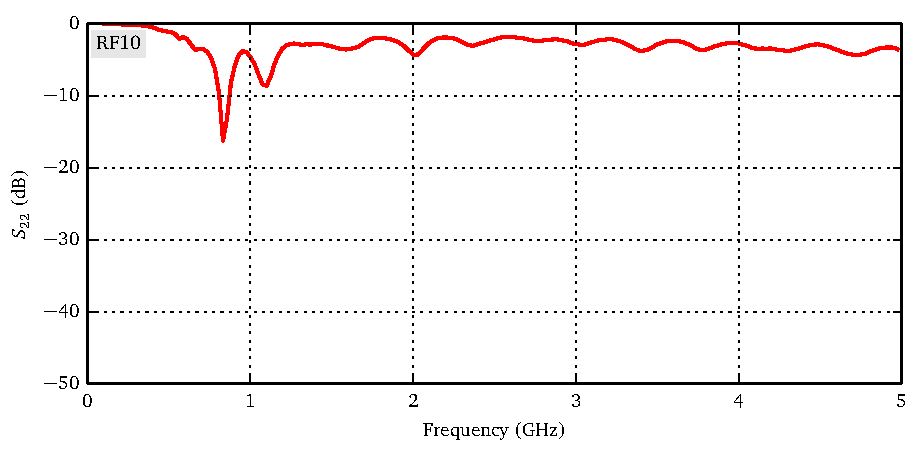
\includegraphics{figs/active/RF10-sParameters.pdf}
 \caption[Experimental $S_{22}$ trace of the RF10 fibre-antenna]
 		{Experimental $S_{22}$ trace for the RF10 fibre-antenna. 
 		The relatively background value of $\sim -4\,\unit{dB}$ indicates
 		that much of the power is reflected back from port 2 (the right-hand side of
 		the antenna, according to our specifications). Also, its single dip at $f\sim800\,\unit{MHz}$
 		is mostly useless for our purposes.}
 \label{fig:active.lcx.rf10sParameters}
\end{figure}

\begin{figure}[h]
 \centering
 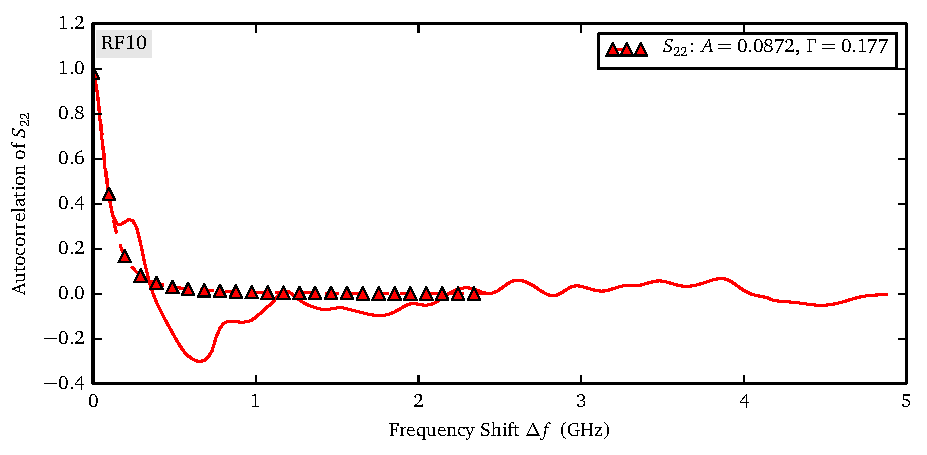
\includegraphics{figs/active/RF10-autoCorrelation.pdf}
 \caption[Autocorrelation of the experimental trace of $S_{22}$ for the RF10 fibre-antenna]
 		{Autocorrelation of the experimental trace of $S_{22}$ for the RF10 fibre-antenna.
 		The dotted line represents the Lorentzian fit. Despite relatively strong negative correlation around $800\,\unit{MHz}$,
 		it is almost zero over the whole interval, but does not fit the Lorentzian.}
 \label{fig:active.lcx.rf10autocorrelation}
\end{figure}

\paragraph{RF21}
The traces of this particular realization shows definite dips, particularly
in the transmission coefficient $S_{12}$, with associated although weaker
dips in both reflection coefficients. The two dips, occurring at $f\sim1.8\,\unit{GHz}$
and $f\sim3.0\,\unit{GHz}$, correspond to optical wavelengths $\lambda_\text{opt}=c/(nf)$ 
of approximately $8.5\,\unit{cm}$ and $5.3\,\unit{cm}$, respectively. They correspond
to the lengths of the first and last scattering cells, approximately; the existence
of these two dips thus seems predicated on the asymmetry of the cells ($d_L\neq d_R$). The fact that all
traces show dips at these frequencies implies that energy is lost in the system. Neglecting
the losses to the metallic layers (they are thinner than the skin depth, minimizing the losses),
we can assume that the lost energy is radiated away through the windows. This design thus 
has two operating frequencies, both outside the desired range, however. 


\begin{figure}[h]
 \centering
 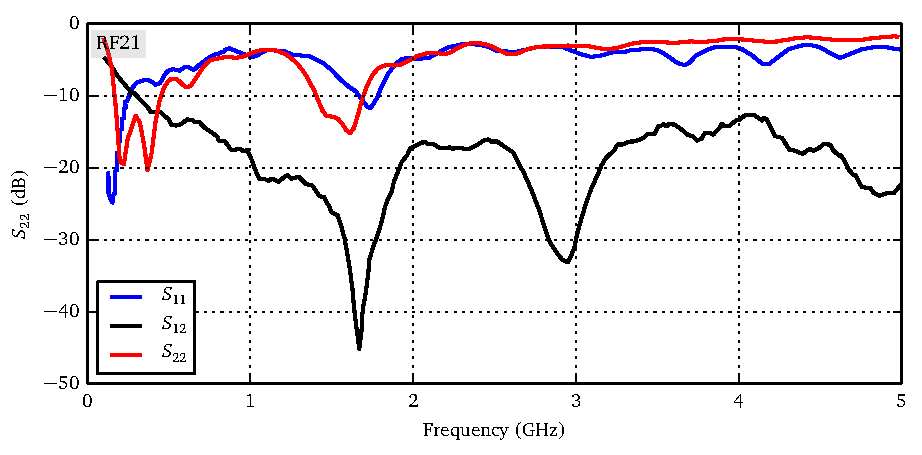
\includegraphics{figs/active/RF21-sParameters.pdf}
 \caption[Experimental $S_{22}$ trace for the RF21 fibre]
 		{Experimental $S_{22}$ trace for the RF21 fibre.}
 \label{fig:active.lcx.rf21sParameters}
\end{figure}

\begin{figure}[h]
 \centering
 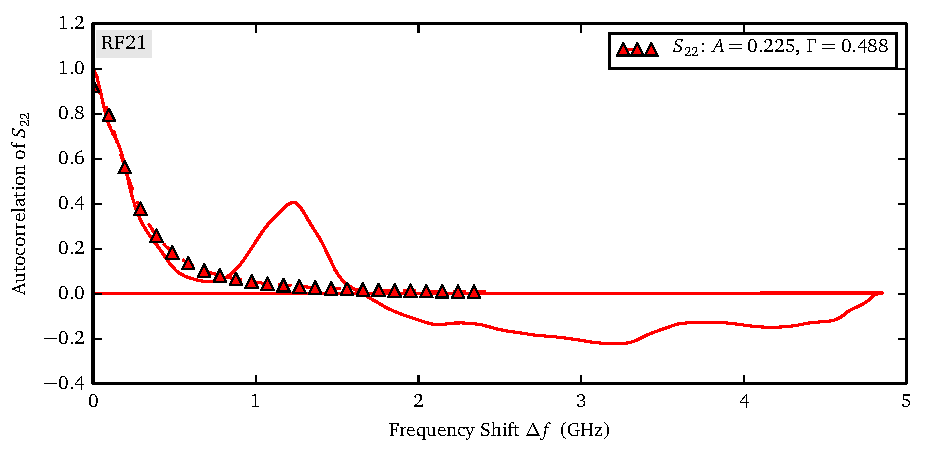
\includegraphics{figs/active/RF21-autoCorrelation.pdf}
 \caption[Autocorrelation of the experimental $S_{22}$ trace for the RF21 fibre-antenna]
 		{Autocorrelation of the experimental $S_{22}$ trace for the RF21 fibre-antenna.}
 \label{fig:active.lcx.rf21autocorrelation}
\end{figure}

\paragraph{RF27 and RF29}
As we can see from Table \ref{tab:active.antennae.rfxx-parameters}, these two antennae
are rather similar. It is thus not surprising that their $S$-parameters
show similar behaviour (compare Figures \ref{fig:active.lcx.rf27sParameters} and
\ref{fig:active.lcx.rf29sParameters}). Their small differences can be explained
away by the experimental variability of both the metal deposition and window
sizing protocols, as they have identical specifications.

Notice the quick decay of the autocorrelation function of the reflection 
coefficients, $S_{11}$ and $S_{22}$. If it were not for the hint of
regularity present in the autocorrelation function of $S_{12}$, 
it could be swiftly concluded that both antennae show chaotic scattering.
In any case, the lack of periodicity in the signals seems to indicate 
that the dip is not due to the geometry of the fibre-antenna. 

\begin{figure}
 \centering
 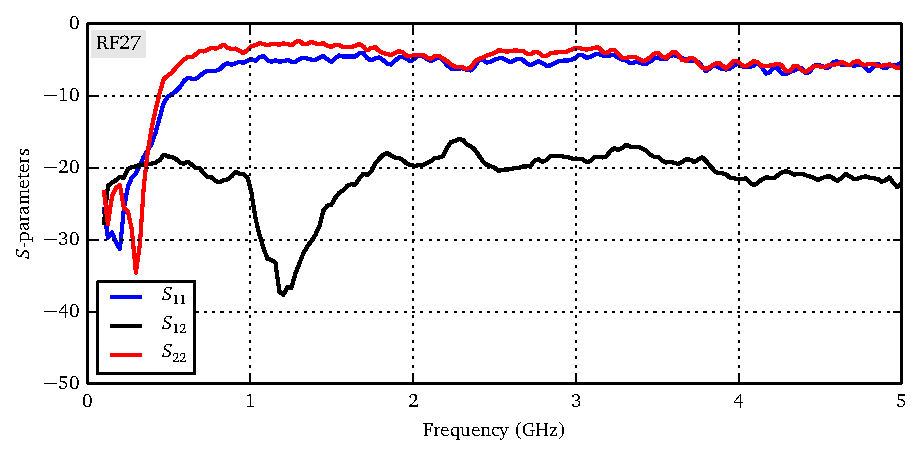
\includegraphics{figs/active/RF27-sParameters.pdf}
 \caption[Experimental $S$-parameter traces for the RF27 fibre-antenna]
 		{Experimental $S$-parameter traces for the RF27 fibre-antenna.}
 \label{fig:active.lcx.rf27sParameters}
\end{figure}

\begin{figure}
 \centering
 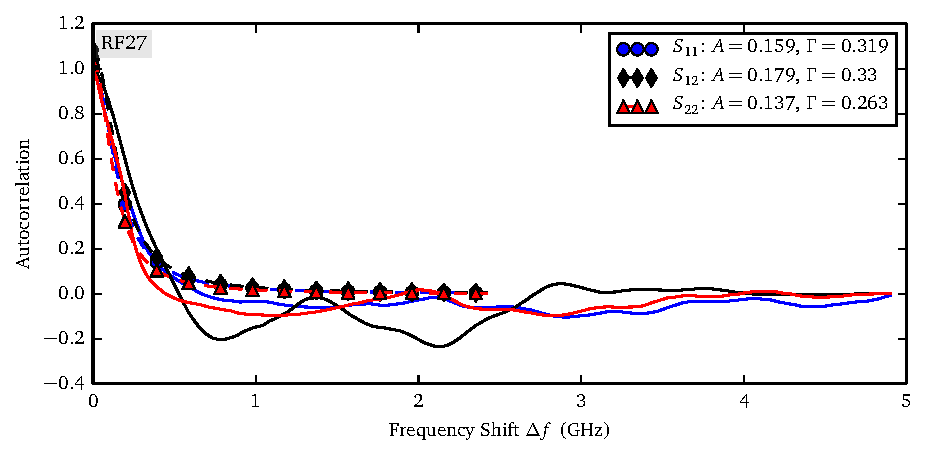
\includegraphics{figs/active/RF27-autoCorrelation.pdf}
 \caption[Autocorrelation of the experimental $S$-parameter traces for the RF27 fibre-antenna]
 		{Autocorrelation of the experimental $S$-parameter traces for the RF27 fibre-antenna.}
 \label{fig:active.lcx.rf27autocorrelation}
\end{figure}


\begin{figure}
 \centering
 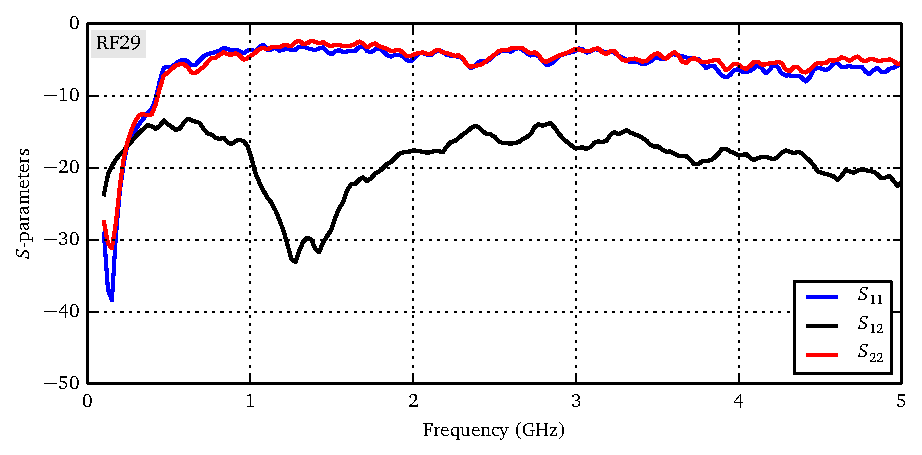
\includegraphics{figs/active/RF29-sParameters.pdf}
 \caption[Experimental $S$-parameter traces for the RF29 fibre-antenna]
 		{Experimental $S$-parameter traces for the RF29 fibre-antenna.}
 \label{fig:active.lcx.rf29sParameters}
\end{figure}

\begin{figure}
 \centering
 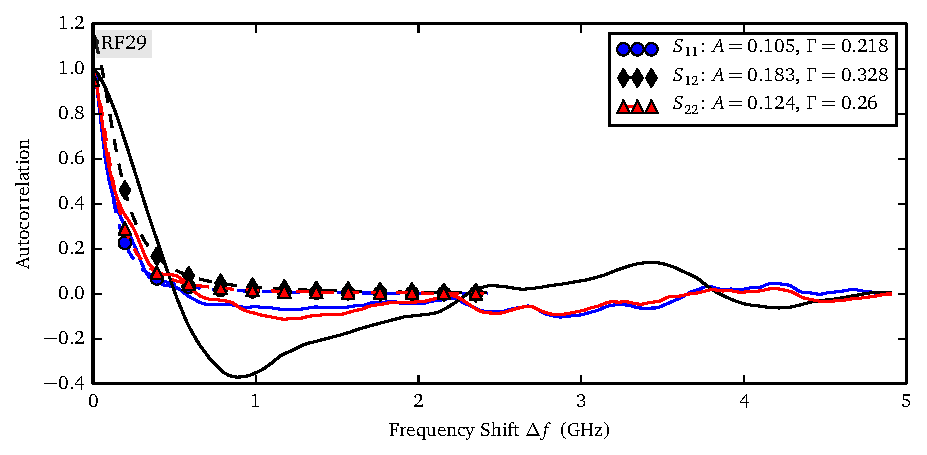
\includegraphics{figs/active/RF29-autoCorrelation.pdf}
 \caption[Autocorrelation of the experimental $S$-parameter traces for the RF29 fibre-antenna]
 		{Autocorrelation of the experimental $S$-parameter traces for the RF29 fibre-antenna.}
 \label{fig:active.lcx.rf29autocorrelation}
\end{figure}

\paragraph{RF33}
The RF33 fibre-antenna, the final antenna produced, is the most mature
one in terms of experimental protocol and is therefore most
worthy of study. Notice that the baseline for this fibre is 
higher than that of the other fibres. The dips also show lower finesse,
although it is possible to make the LCX operate as an antenna
at some of the frequency dips. Specifically, there is a dip at
$f\sim2.6\,\unit{GHz}$, which is close to our requirements. 
There is however, an increase in the reflection coefficients
at this frequency, hinting that the antenna might not be 
efficient at that frequency. There seems to be a repetition 
of the trace at every $2\,\unit{GHz}$. 

The autocorrelation of the trace of $S_{22}$ shows a strong
periodic component, which we have isolated by taking the 
FFT of the signal. 

We have also taken the Fourier transform of the experimental
and simulation data (for $\delta_1=0$). To our discontent, 
it seems that the datasets do not share periodic properties. 
Figure \ref{fig:active.lcx.rf33fft} shows the intensity
of the FFT transform. To see if the periodic components corresponded
to particular lengths in the system, we converted the associated
wavelengths to frequencies and plotted them as vertical lines in the figure. 
$f_1$ is the fundamental mode of infinite \gls{lcx} \cite{WAN2001}, namely
  \begin{equation}
   f_1 = \frac{c}{\left(S_z+d_z\right)\left(\sqrt{\epsilon_\text{Si}}+1\right)} \sim 1.6\,\unit{GHz}.
  \end{equation}
The frequency associated with the optical and the actual lengths of the window
are
  \begin{align*}
   l_\text{opt}	&= \frac{c}{S_z\sqrt{\epsilon_\text{Si}}} \sim 4.5\,\unit{GHz}	\\
   l_\text{phy}	&= \frac{c}{S_z} \sim 8\,\unit{GHz}.
  \end{align*}

Nothing thus far seems to explain the periodic properties of the 
experimental $S_{22}$ trace, although it might just be that 
$f_1$ depends on the sizes $d_L$ and $d_R$ and what we see is
the fundamental mode of our quasi-LCX. 

\begin{figure}
 \centering
 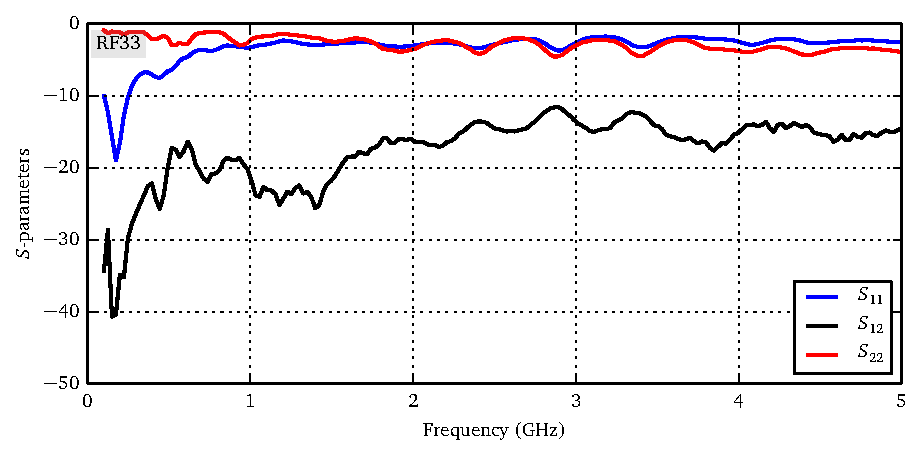
\includegraphics{figs/active/RF33-sParameters.pdf}
 \caption[Experimental $S$-parameter traces for the RF33 fibre-antenna]
 		{Experimental $S$-parameter traces for the RF33 fibre-antenna.}
 \label{fig:active.lcx.rf33sParameters}
\end{figure}

\begin{figure}
 \centering
 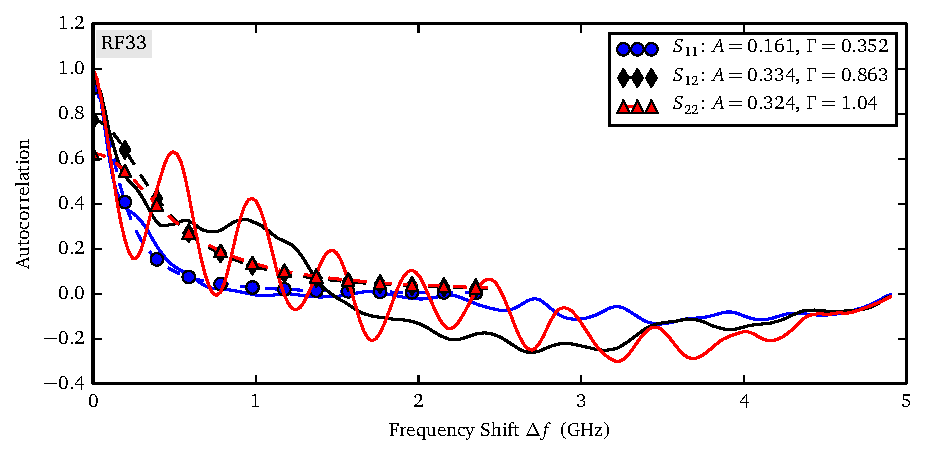
\includegraphics{figs/active/RF33-autoCorrelation.pdf}
 \caption[Autocorrelation of the experimental $S$-parameter traces for the RF33 fibre-antenna]
 		{Autocorrelation of the experimental $S$-parameter traces for the RF33 fibre-antenna.}
 \label{fig:active.lcx.rf33autocorrelation}
\end{figure}

\begin{figure}
 \centering
 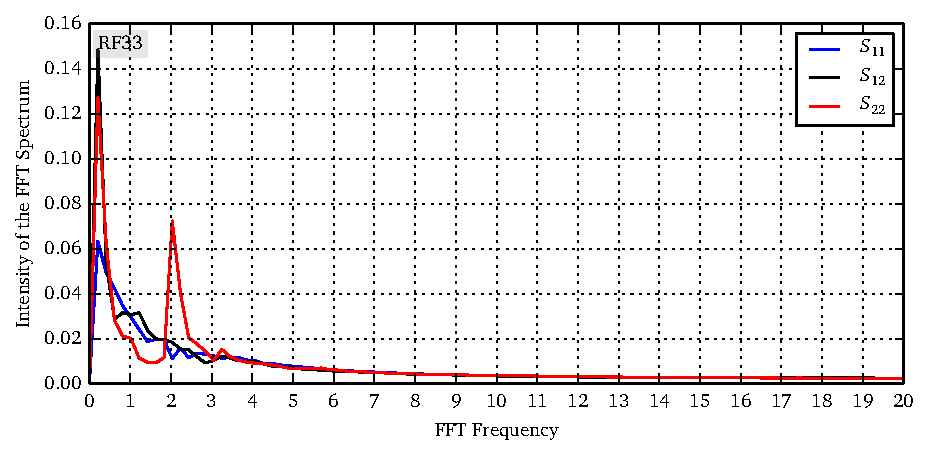
\includegraphics{figs/active/RF33-fft.pdf}
 \caption[FFT spectrum of the autocorrelation functions of the $S$-parameters of the RF33 fibre-antenna]
 		{FFT spectrum of the autocorrelation functions of the $S$-parameters of the RF33 fibre-antenna.}
 \label{fig:active.lcx.rf33fft}
\end{figure}


\subsubsection{Comparison with Simulation Results}
The specifications of each RFxx was based on the numerical simulation
of the antennae. However, once they were built, it became clear the 
numerical modeling did not correlate well with the experimental
realizations. As we will see, the experimental traces rarely possessed
the same features as the numerical ones and the far-field patterns 
did not match. 

The main cause for such poor agreement between theory and experiment
was hypothesized to be related to the metallic layers. As discussed
above, the experimental method the group used did not allow for any
control over the thickness of metal deposited, and did not guarantee
its mechanical properties nor its chemical ones. In other words, 
the layers could be grainy and contain impurities. The former was taken
into account directly in the HFSS software, as the ``Layered Impedance
Boundary Conditions'' module allows for inhomogeneities in the surfaces.
The author of this essay thus tried to model the effects of impurities 
on the conductivity and the effect of the resulting small thicknesses
of the layers. The next section details the modeling efforts.  

\paragraph{Preliminary Results}
Because of its easily interpretable traces and of its (at the time)
quality, the RF21 fibre is the one we analyze. Figure
\ref{fig:active.lcx.rf21sParameters-sim} shows both the experimental traces
and the numerically predicted ones. Note that this simulation did not contain
any effective boundary conditions, but assumed that the silver layers had a 
constant $2\,\unit{\mu m}$ thickness. We can see transmission-line behaviour
in the $S_{12}$ parameter, as the wave is transmitted without much loss
regardless of frequency. Clearly, this model does not represent reality
well. Removing the silver layers and replacing them by effective boundary
conditions does not solve the problem, as is shown in Figure 
\ref{fig:active.lcx.rf21sParameters-concSweep}. 

\begin{figure}
 \centering
 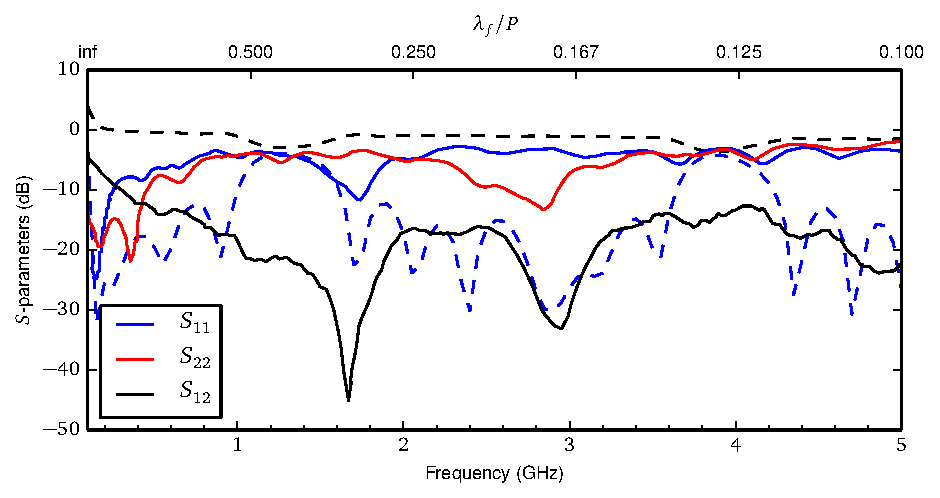
\includegraphics[width=\textwidth]{figs/active/sParametersRF21.pdf}
 \caption[$S$-parameters of the RF21 fibre design]
 		{$S$-parameters of the RF21 fibre design. The full lines represent
	  	the experimental data while the dotted lines represent the simulation data.
	  	The top $x$ axis shows the $S$-parameters as a function of the ratio of the 
	  	vacuum wavelength $\lambda_f$ over the period of the windows $P$.}
 \label{fig:active.lcx.rf21sParameters-sim}
\end{figure}

AFM pictures (see Figure \ref{fig:active.lcx.AFM})  have suggested that the deposited
metal is in fact a mixture of silver and silver oxide. To evaluate
the effective conductivity of the mixture, we have used Bruggeman's model \cite{LAN1978}.
The model starts from a homogeneous medium, call it medium 1, 
of conductivity $\sigma_1$ and replaces spherical portions of this material 
by another one of conductivity $\sigma_2$. When this process is done, 
we are left with a inhomogeneous material with partial concentrations $\delta_i$
of each material. The effective conductivity $\sigma_e$ of the medium can be computed
using the relation (for an arbitrary number of materials)
  \begin{equation}
    \sum_i^n \delta_i \frac{\sigma_i-\sigma_e}{\sigma_i+(d-1)\sigma_e} =0 
  \end{equation}
where $\sum_i\delta_i=1$ and $d$ is the dimensionality of the system.
Solving for $\sigma_e$ in the case $n=2$ yields
  \begin{equation}
   (d-1)\sigma_e^2+\left[\left(d\delta_1-1\right)\sigma_1+\left(d\delta_2-1\right)\sigma_2\right]+\sigma_1\sigma_2=0.
  \end{equation}
The positive solution is, defining $q=\left(d\delta_1-1\right)\sigma_1+\left(d\delta_2-1\right)\sigma_2$
  \begin{equation}
   \label{eq:antenna:bruggeman}
   \sigma_e = \frac{1}{2d-2}\left[q+\sqrt{q^2+4(d-1)\sigma_1\sigma_2}\right].
  \end{equation}
Using this effective conductivity in \eqref{eq:active.antennae.thickGeneralEquations} yields 
the associated thicknesses. 

\begin{figure}
 \centering
 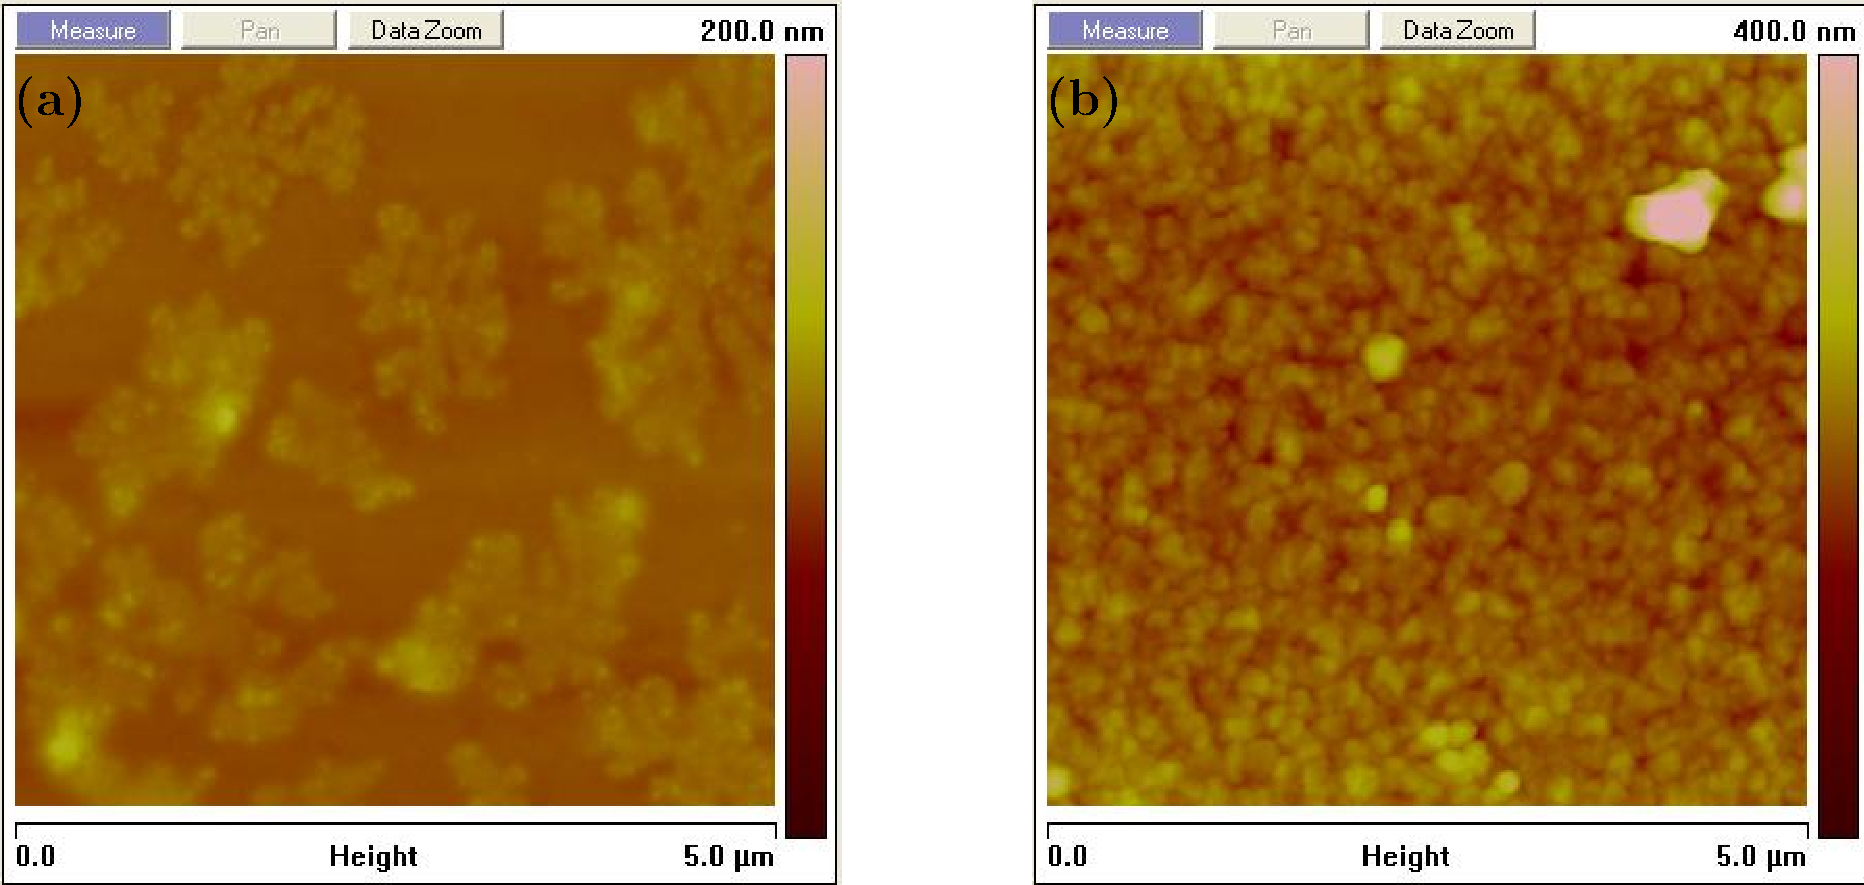
\includegraphics[width=0.8\textwidth]{figs/active/out/AFM.pdf}
 \caption[AFM pictures of silver deposited onto glass plates]
 		{AFM pictures of silver deposited onto glass plates. \textbf{(a)} Flakes of silver oxide seem to be forming onto the deposited
	  	silver layer. \textbf{(b)} Sample image showing the inhomogeneity of the
	  	silver layer.}
 \label{fig:active.lcx.AFM}
\end{figure}

It also came to light that the conductivity 
of thin metal films can be a function of their thicknesses. 
The state-of-the-art model to describe this dependence is the 
\textit{Fuchs-Sondheimer} model, which essentially computes the 
electron distribution in the metal as a function of its thickness. 
From Ohm's law, it is then trivial to obtain the value of the 
conductivity \cite{FUC1938,SON1952,PUR2007}. The general relationship
is
	\begin{multline}
		\frac{\sigma_F}{\sigma_0} = 
			1-\frac{3(1-p)}{8\kappa}\\+\frac{3}{4\kappa}\left(1-p\right)^2
			\sum_{\nu=1}^\infty p^{\nu-1}
			\left\{
				\int_{\kappa\nu}^\infty\frac{e^{-\xi}}{\xi}d\xi\left(\kappa^2\nu^2-\frac{\kappa^4\nu^4}{12}\right)
				+e^{-\kappa\nu}\left(\frac{1}{2}-\frac{5\kappa\nu}{6}-\frac{\kappa^2\nu^2}{12}+\frac{\kappa^3\nu^3}{12}\right)	
			\right\}
	\end{multline}
where $\kappa=t/\lambda_0$ where $\lambda_0$ is the mean free path of the electrons in the metal and
$t$ the thickness of the sample. The parameter $p$ is the proportion of electrons that are reflected
elastically at the boundary. For rough edges, we expect the electrons to be scattered off randomly 
and thus $p\sim0$. Notice that the above expression is extremely unwieldy and yields to a highly
non-linear root search when substituted in \eqref{eq:active.antennae.thickGeneralEquations}. 
We will use the much more convenient form 
  \begin{equation}
      \sigma_F = \frac{\sigma_0}{1+\frac{3\lambda}{8d}\left(1-p\right)}
  \end{equation}
which leads to a simpler cubic equation for the thickness.
This model states that conductivity
diminishes as the thickness of the metallic layer gets smaller, 
as one would expect.

In Figure \ref{fig:antenna.thicknessRatios}, we compare the 
thicknesses obtained via the bulk conductivity model (Bruggeman 
effective conductivity) and the Fuchs-Sondheimer model with 
effective conductivity for the RF33 fibre. Given that the AFM pictures
show surface inhomogeneity, we assume diffuse scattering in 
the FS model ($p=0$). We see that choosing a dimensionality 
of 3 or 2 does not significantly affect the thicknesses, but
we see a difference of about 20\% in the effective conductivities.

The most interesting thing, though, is that the FS
model predicts metallic layers that are 10\% to 80\% thicker 
than with the bulk conductivity model. 

\begin{figure}
  \centering
  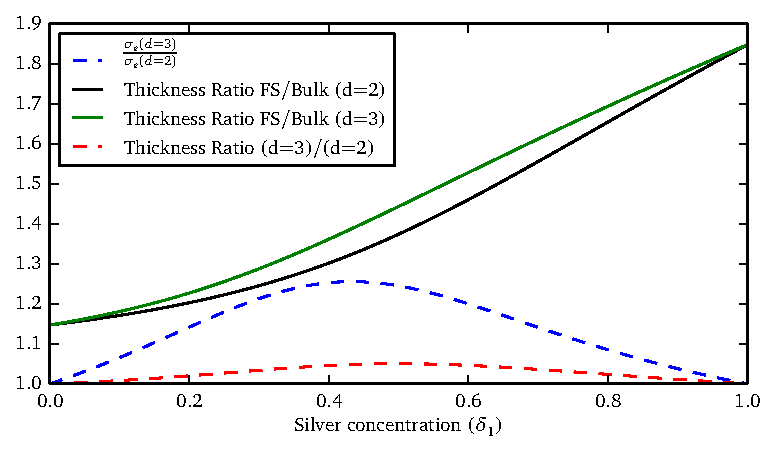
\includegraphics[width=0.9\textwidth]{figs/active/comparisonThickness.pdf}
  \caption[Thickness ratios as a function of the silver concentration]
	  {We show multiple ratios as a function of the silver concentration,
	  $\delta_1$. The blue line shows the ratio between the effective
	  conductivities for a choice of $d=2$ and $d=3$. The black and 
	  green lines show the ratio of the thickness predicted by using
	  the Fuchs-Sondheimer conductivity in Eq. \eqref{eq:antenna:thickGeneralEquations}
	  to the thickness predicted by using the bulk conductivity.
	  The red line shows the ratio of the green line to the black line.}
  \label{fig:antenna.thicknessRatios}
\end{figure}

We have simulated the RF21 fibre using Bruggeman's model
for the effective conductivity and with values
of $\delta_1\in\{0,1\}$ and $d=3$ in \eqref{eq:antenna:bruggeman}.
After obtaining the simulated $S_\text{11}$ parameter of the fibre,
we compared it to the experimentally obtained one using the Pearson
correlation coefficient. For two samples $\{X_i\}$ and 
$\{Y_i\}$, it is defined as
  \begin{equation}
    r = \frac{\sum_i^n\left(X_i-\left\langle X\right\rangle\right)\left(Y_i-\left\langle Y\right\rangle\right)}
	     {\sqrt{\sum_i^n\left(X_i-\left\langle X\right\rangle\right)^2}\sqrt{\sum_i^n\left(Y_i-\left\langle Y\right\rangle\right)^2}}.
  \end{equation}
From the definition, we see that the simultaneous linear transformations $X_i\rightarrow b+aX_i$ and $Y_i\rightarrow d+cY_1$
do not change the value of the Pearson coefficient. This means that even if the two samples
do not have the same normalization or are shifted by a constant amount, the correlation 
will stay the same. As such, the Pearson correlation measures the degree at which 
both samples are linearly related. 

Figure \ref{fig:active.lcx.rf21sParameters-sim} shows the experimental and simulated
$S_{11}$ parameter. At first look, it might seem like the general form 
of the curves are similar, but our quantitative analysis will show 
that that would be wrong. To make sure that our simulation data was not simply
shifted in frequency due to an small error in the geometry, we have
also calculated the correlation for a shifted dataset 
\footnote{To do so, we simply right-shifted the arrays containing
the simulation data and removed the data that fell outside the frequency range 
of the experimental data.}. This changes
the Pearson correlation because we must elide some of the experimental
and simulation data to do so. Figure \ref{fig:antenna.shiftCorrelation}
shows our results. We see that there are little to no correlation
between the simulation data and the experimental data with $r\in\{-0.04,0.05\}$. 

\begin{figure}
 \centering
 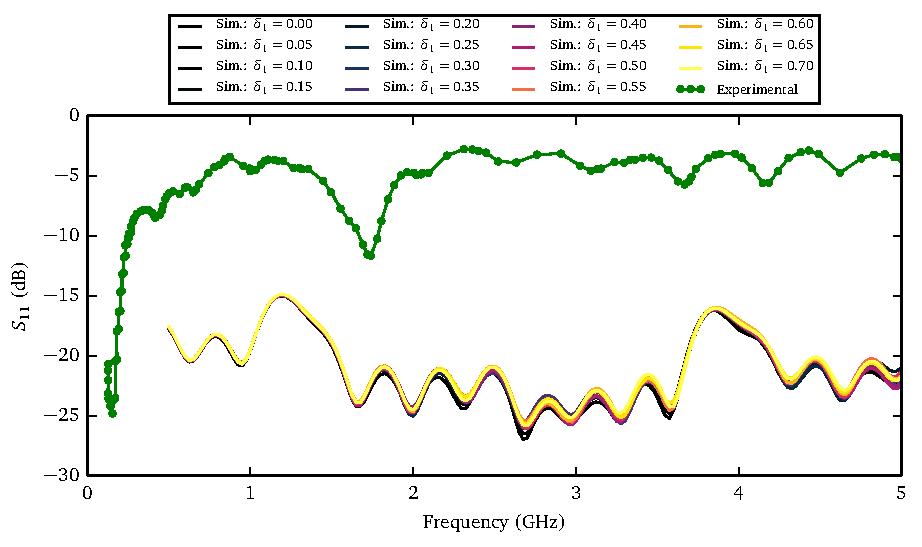
\includegraphics[width=0.8\textwidth]{figs/active/sParameters-concSweepS11.pdf}
 \caption[Experimental and simulated $S_{11}$ parameter for the RF21 fibre]
	 {Experimental and simulated $S_{11}$ parameter for the RF21 fibre.}
 \label{fig:active.lcx.rf21sParameters-concSweep}
\end{figure}

\begin{figure}
 \centering
 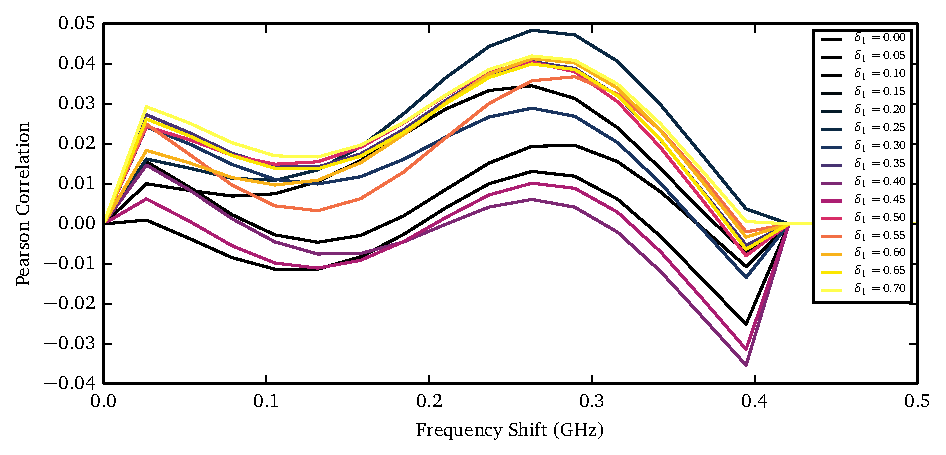
\includegraphics[width=0.8\textwidth]{figs/active/shiftCorrelationS11.pdf}
 \caption{Pearson correlation coefficient as a function of the frequency
	  shift of the data.}
 \label{fig:antenna.shiftCorrelation}
\end{figure}

We unfortunately conclude this section by noting that the above phenomena
are not sufficient to explain the lack of correlation between the experimental
and simulation datasets. The models do predict dramatically different properties
for the metallic layers, but it seems that this does not affect the $S$-parameters
all that much. One explanation is that the effect of the surface inhomogeneities
are \textit{not} taken into account when computing the thicknesses. By using a
\textit{ad hoc} model to compute the effects of randomly distributed inhomogeneities
on the base conductivity $\sigma_0$ of the metallic layers \cite{CUR2012}, one could obtain a better
estimate of the thicknesses and possibly a better fit between the experimental and simulated datasets.

We can see, however, that while of the details of the $S$-parameters are not well reproduced, some
dips appear both in experimental and simulated traces. The irregular scattering, due to the experimental
variations of the geometry, could account for the suppression of some dips and the possible shifts. 
However, it is difficult to predict \textit{a priori} which ones will be suppressed and which ones will
be shifted, as we do not have ``robustness'' information. 
% !TeX root = ../msc_thesis_jayd.tex
\chapter{Conclusion}
\epigraph{Qui va ça et là finit par arriver.}{Wisdom of a Fortune Cookie}
\section{Summary}
We have presented some results about the modelization of bidimensional
resonators, both passive and active, and have designed a leaky coax
antenna for smart textile applications. 

Throughout this essay, we have made use of the \gls{sMatrix} formalism
to compute the resonances of the devices under study. For passive
(and lossless) cavities, the formalism was augmented by the
introduction of the time-delay matrix, or \gls{qMatrix}, which
is related to the overlap of the normal modes of the resonator.
The eigenvalues of this matrix turned out to be related to the
poles of the \gls{sMatrix} and be composed of a sum of Lorentzian
curves.  The eigenvalues were in fact the time-delays associated with
the interaction of the incoming light field with the scatterer. 
The eigenvectors of the \gls{qMatrix} describe a set of modes that exist for
every continuous value of $k$. The set of modes has the property of 
interacting in a \textit{self-replicating} manner with the cavity. 
While the interaction does not disturb the angular momentum distribution,
it incurs a phase shift on the incoming field, and the energy derivative
of this shift is the time-delay suffered by the mode. It can be directly
related to the $Q$-factor of the mode. The introduction of the 
\gls{qMatrix} transforms the search for the poles of the \gls{sMatrix}
in the complex plane in a search for the maxima of the time-delay spectrum
on the real $k$-line.

The properties of the \gls{qMatrix}, and its simple interpretation, 
mostly depend on the unitarity of the \gls{sMatrix}. When the 
potential is complex, this is no longer true. It is however still
possible to define a Hermitian \gls{qMatrix} with the sought-after properties,
but it requires the evaluation of the \gls{qMatrix} along a curve in 
the complex $k$-plane. This makes the interpretation of the spectrum
of $\mat{Q}$ as a time-delay more difficult, and most importantly 
makes their relationship with the poles of the \gls{sMatrix} clouded.
It also nullifies the computational advantages of working with $k\in\mathbb{R}$.
The author thus concluded that for active (or lossy) cavities, it is best
to stick with the \gls{sMatrix} alone. 

This seemed a perfect segue into the study of active cavities, where
the SALT is used to model the effect of a quantum gain medium as
an additional term in the refractive index\footnote{This is valid for the TM
mode only.}. The latter is dispersive and complex, possibly non-linear.
This motivated the development of a more stable numerical method. 
We used a Lippmann-Schwinger approach. The method is calibrated using
the homogeneous circular cavity laser and we discuss the pole structure
of the scattering matrix.

We then turn our attention to the design of a LCX antenna. The complex
geometry of the antenna and the perplexing features of the metallic
layers made for a complicated modeling task. Some attempts were made
at explaining the major discrepancies between the experimental
and simulation datasets. We quantified the effects of mixing
different materials and of thin films using the Bruggeman
and Fuchs-Sondheimer models, respectively. Using FEM software
to incorporate these models, as well as taking into account
possible surface inhomogeneities via a dedicated module in the
software, the author concluded that an \textit{ab initio}
model of the effect of the surface inhomogeneities was needed
in order to properly assess the thicknesses of the silver layers.

This last paragraph should convince the reader that data alone is 
not sufficient to explain everything. The first section showed that
theory can give both qualitative and quantitative insight into
the systems under study. Data is of course necessary to confirm 
or infirm theory, but, for intellectual and practical reasons, cannot
stand alone. The intellectual exercise of probing the working of the 
universe, in itself, better the state of our knowledge. The resulting
theories provide guidelines for future research and new experiments
\footnote{Guidelines that must sometimes be broken, of course \cite{KUH1996}.}
and ease the interpretation of the data. On the more practical side, the 
guidelines can dramatically reduce the cost of the design phase of 
any kind of device. 

\section{Perspectives}
While most of this essay limited its scope to bidimensional cavities, 
many of the tools can be directly generalized to three dimensions. Much
work was done by the author to find methods that would work reasonably
well in 3D, but it was never seen to completion. The last appendix of this
essay presents some of the basic tools for 3D scattering. They are published
here in the hope that they may be useful in the future. 

One of the main approximations generally used in the study of microcavities
in the assumption that the fields exist in infinitely long cylinders. 
This works reasonably well, but is not enough for accurate comparison with 
experiments. One interesting project would be to use a full 3D numerical
method and investigate the 2D limit of electromagnetism in microcavities, 
if it is well-defined. This could in turn be used to properly model 
polarization effects, which could perhaps be put to use as an 
extra degree of freedom in biodetection devices.

\section{Technical Acknowledgements}
This work would not have been possible without \cite{SAN2010}, a C++ linear algebra
library. We also wish to thank \cite{GEI2013} for the color-blind compliant color maps.

% -------------------- Appendices ---------------------	%
% Due to the technical nature of the work done, the 	%
% appendices mostly contain derivations and notes on 	%
% numerical implementations of algorithms.				%
% -----------------------------------------------------	%
\appendix
% !TeX root = ../msc_thesis_jayd.tex
\chapter{Bessel Functions}
This appendix contains some results concerning the 
Bessel functions. Given our redution of Maxwell's equations 
from 3D to 2D using cylindrical coordinates, the 
Bessel functions will form the basis of our analysis, 
as they are the eigenfunctions of
Helmholtz's equation in those coordinates.

We thus wish to collect some of their most important
properties here for easy reference. Most of them come from the celebrated
volume by Abromowitz \& Stegun \cite{ABR1965}, while a few
come from \cite{CUY2008}. Proper reference will be given when needed. 

In what follows, $\nu,z\in\mathbb{C}$ and $n\in\mathbb{N}$ unless explicitly
stated otherwise.

\section{Definition and Elementary Properties}

\subsection{Differential Equation}
The Bessel functions solve the differential equation
  \begin{equation}
   \label{eq:app.Bessel.diffEquation}
   z^2\frac{d^2w}{dz^2}+z\frac{dw}{dz}+(z^2-\nu^2)w=0
  \end{equation}
which is a special case of the confluent hypergeometric
differential equation, which is in turn a special case
of the hypergeometric differential equation. When solved
via Fröbenius' method, it yields the solution
  \begin{equation}
   \label{eq:app.Bessel.seriesJ}
   J_\nu(z) = \sum_{k=0}^\infty \frac{(-1)^k\left(\frac{1}{2}z\right)^{\nu+2k}}{k!\Gamma(\nu+k+1)}.
  \end{equation}
This is the Bessel function of the first kind. A second, linearly independant
is defined by
  \begin{equation}
   Y_\nu(z) = \frac{J_\nu(z)\cos\pi\nu-J_{-\nu}(z)}{\sin\pi\nu}
  \end{equation}
where a valid limiting process must be used when $\nu\rightarrow n$. 

We will be mostly interested in a second set of linearly independant
solutions: the Hankel functions. They are defined by 
  \begin{subequations}
  \label{eq:app.Bessel.hankelDef}
  \begin{align}
   H_\nu^{(+)}(z)	&= J_\nu(z)+iY_\nu(z)	\\
   H_\nu^{(-)}(z)	&= J_\nu(z)-iY_\nu(z).
  \end{align}
  \end{subequations}
We will alternatively use the notation
  \begin{equation}
   H_\nu^{(\omega)} = J_\nu(z)+i\omega Y_\nu(z)\qquad (\omega=\pm)
  \end{equation}
to denote both functions at the same time.

\subsection{Recurrence Relations}
From the differential equation itself, we can derive multiple
recurrence relations that the whole family of Bessel functions 
obey. If $\mathcal{C}$ denotes $J$, $Y$, $H^{(\pm)}$ or any 
linear combination of the four functions, we have
  \begin{subequations}
  \begin{align}
   \mathcal{C}_{\nu-1}(z)+\mathcal{C}_{\nu+1}(z)		&= \frac{2\nu}{z}\mathcal{C}_\nu(z)	\label{eq:app.Bessel.recurrenceBessel}\\
   \mathcal{C}_{\nu-1}(z)-\mathcal{C}_{\nu+1}(z)		&= 2\mathcal{C}_\nu'(z)			\label{eq:app.Bessel.recurrenceDiffBessel}\\
   \mathcal{C}_{\nu-1}(z)-\frac{\nu}{z}\mathcal{C}_\nu(z)	&= \mathcal{C}_\nu'(z)			\\
   -\mathcal{C}_{\nu+1}(z)+\frac{\nu}{z}\mathcal{C}_\nu(z)	&= \mathcal{C}_\nu'(z).
  \end{align}
  \end{subequations}
However, the minimal solution to these recurrence relations is 
$J_\nu(z)$, so any attempt at numerically evaluating $Y$ or $H_\nu^{(\pm)}$
using these is foiled (see \S\ref{sec:app.numTools.logDeriv} for details). 

\subsection{Relations between Solutions}
The following are analytical relationships between the set of 
Bessel functions. They can be of use in both standard and numerical 
analysis. 

\begin{description}
 \item Reflection Formulas \cite[p.~286]{PRE2007}
  \begin{subequations}
  \begin{align}
   J_{-\nu}(z)	&= \cos\nu\pi J_\nu(z)-\sin\nu\pi Y_\nu(z)	\\
   Y_{-\nu}(z)	&= \sin\nu\pi J_\nu(z)+\cos\nu\pi Y_\nu(z)	\\
   J_{-n}(z)	&= (-1)^nJ_n(z)					\\
   Y_{-n}(z)	&= (-1)^nY_n(z)					\\
   H_{-\nu}^{(\omega)} &= e^{i\omega\nu\pi}H_\nu^{(\omega)}
  \end{align}
  \end{subequations}
 \item Complex Conjugate ($\nu\in\mathbb{R}$)
  \begin{subequations}
  \begin{align}
   \overline{J_\nu(z)}	&= J_\nu(\overline{z})	\\
   \overline{Y_\nu(z)}	&= Y_\nu(\overline{z})	\\
   \overline{H_\nu^{\omega}(z)} &= H_\nu^{(-\omega)}(\overline{z})\label{eq:app.Bessel.conjHankel}
  \end{align}
  \end{subequations}
\end{description}

The last of these equations is of particular importance in establishing
symmetries of the scaattering matrix.

\section{Asymptotic and Limiting Forms}
\subsection{Expansions for Small Arguments and Fixed $\nu$}\label{sec:app.Bessel.smallArguments}
From the first few terms of the power series \eqref{eq:app.Bessel.diffEquation}, 
  \begin{equation}
    J_\nu(z) = \frac{1}{\Gamma(\nu+1)}\left(\frac{z}{2}\right)^\nu\left[1-\frac{1}{\nu+1}\left(\frac{z}{2}\right)^2\right]+\mathcal{O}(z^{\nu+4}).
  \end{equation}
  
Using the first terms of the ascending series for integer orders $n$ \cite[\S9.1.11]{ABR1965}
  \begin{multline}
   Y_n(z)=-\frac{1}{\pi}\left(\frac{z}{2}\right)^{-n}\sum_{k=0}^{n-1}\frac{(n-k-1)!}{k!}\left(\frac{z}{2}\right)^{2k}
      +\frac{2}{\pi}\ln\frac{z}{2}J_n(z)
      \\-\frac{1}{\pi}\left(\frac{z}{2}\right)^n\sum_{k=0}^\infty\left\{\psi(k+1)+\psi(n+k+1)\right\}\left(\frac{z}{2}\right)^{2k}\frac{1}{k!(n+k)!},
  \end{multline}
where 
  \begin{equation}
   \psi(n+1) = -\gamma +\sum_{k=1}^nk^{-1}\qquad(\gamma=0.57721\,56649\ldots)
  \end{equation}
is the digamma function. The cases $n=0$ and $n\neq0$ differ
  \begin{align}
   Y_0(z)	&= \frac{2}{\pi}\left(\ln\frac{z}{2}+\gamma\right)+\mathcal{O}(z^2)	\\
   Y_n(z)	&= -\frac{(n-1)!}{\pi}\left(\frac{z}{2}\right)^{-n} +\mathcal{O}(z^{-n+2}).
  \end{align}

The expansions of the Hankel functions is found by using 
their definition \eqref{eq:app.Bessel.hankelDef}:
  \begin{align}
   H_0^{(\omega)}(z)	&=1+\frac{2i\omega}{\pi}\left(\ln\frac{z}{2}+\gamma\right)+\mathcal{O}(z^2)	\\
   H_n^{(\omega)}(z)	&=-\frac{i\omega(m-1)!}{\pi}\left(\frac{z}{2}\right)^{-n}+\mathcal{O}(z^{-n+2}).
  \end{align}

\subsection{Expansions for Large Arguments and Fixed $\nu$}
The Bessel functions, jealous of the simpler trigonometric functions, 
try to mimic them when their arguments get large. We have
  \begin{subequations}
  \begin{align}
   J_\nu(z)		&\approx \sqrt{\frac{2}{\pi z}}\cos\left(z-\frac{\nu\pi}{2}-\frac{\pi}{4}\right)	\\
   Y_\nu(z)		&\approx \sqrt{\frac{2}{\pi z}}\sin\left(z-\frac{\nu\pi}{2}-\frac{\pi}{4}\right)	\\
   H_\nu^{(\omega)}(z)	&\approx \sqrt{\frac{2}{\pi z}}e^{i\omega\left(z-\frac{\nu\pi}{2}-\frac{\pi}{4}\right)}\label{eq:app.Bessel.asymptoticHankel}
  \end{align}
  \end{subequations}
The last of these makes the respect of Sommerfeld's radiation condition a breeze in cylindrical coordinates.
% !TeX root = ../msc_thesis_jayd.tex
\chapter{Numerical Methods}
In this appendix, we review the details of some of the numerical
methods and tools described in the essay. Most of the sections
concern the numerical computation of the scattering matrix, 
as it is our main object of interest.

We wish to solve Helmholtz's equation
	\begin{subequations}
	\label{eq:sec.numMethods.mainEquations}
	\begin{align}
		\left[\nabla^2+k^2n_0^2\right]\ket{\psi}	& =0					& \bo{r}\notin\mathcal{C}	\\
		\left[\nabla^2+k^2n_c^2\right]\ket{\psi}	& =V(\bo{r})\Ket{\psi}	& \bo{r}\in\mathcal{C}
	\end{align}
where we write the exterior solution ($\bo{r}\notin\mathcal{C}$) as $\ket{\psi}=\ket{\psi^\text{inc}}+\ket{\psi^\text{sca}}$
and the interior solution as $\ket{\psi}=\ket{\psi^i}$. The potential operator has the form
	\begin{equation*}
		V(\bo{r}) = \frac{2}{n}\nabla n\cdot\nabla\{\}
	\end{equation*}
in TE polarization, but vanishes in the TM one. Together with the transmission conditions
	\begin{align}
		\ket{\psi^i} 						& = \ket{\psi^\text{inc}}+\ket{\psi^\text{sca}} 							& \bo{r}\in\partial\mathcal{C}	\\
		\eta_c^2\frac{d\ket{\psi^i}}{dn}	& = \eta_o^2\frac{d}{dn}\left(\ket{\psi^\text{inc}}+\ket{\psi^\text{sca}}\right) &\bo{r}\in\partial\mathcal{C},
	\end{align}
	\end{subequations}
where $\eta_i = 1\,(1/n_i^)$ in the TM (or TE) polarization, 
these equations form the general scattering problem for 2D microcavities. 

The scattering matrix depends on the various parameters defined above. The environment
is considered to be infinite and featureless, i.e. $\mathcal{C}^c=\mathbb{R}^2$ and 
$n_0$ is a constant. The cavity region, $\mathcal{C}$, can be any bounded, connected set
(or a collection of such sets) and endowed with a refractive index $n_c=n_c(r,\theta)$, 
which is allowed to a function of position and frequency. The support of the function 
$n_o^2-n_c^2$ coincides with the cavity region $\mathcal{C}$. The scattering operator 
is defined by the relationship
	\begin{equation}
		\Ket{\psi^\text{sca}} = \mathcal{S}\Ket{\psi^\text{inc}}
	\end{equation}
and relates incoming parts of the field to the outgoing ones \textit{outside}
of the \gls{lss}, outside of the support of $n_o^2-n_c^2$.

\section{Numerical Computation of the Scattering Matrix in SQA}\label{sec:app.numTools.scatMat}
Since it is our primary tool, we will describe the numerical implementation
of the \gls{sqa} in detail. The necessary notation and parameters are defined in 
Figure \ref{fig:passive.numerical.radialDiscretization}. The discretization
contains three distinct regions; an inner circle of radius $r_0$ (let us call it
the first scattering surface, or FSS), the outer circle of radius $R_0$ (the \gls{lss})
and the region in between, which is discretized in onion-like shells. We suppose
that refractive index in the FSS is constant and equal to $n_\text{in}=n_c(0,0)$. 
The differential equation inside the FSS reduces to the Bessel equation 
\eqref{eq:app.Bessel.diffEquation}. The solution is thus given by 
\eqref{eq:passive.formalism.innerCircleSoln}. In the outer region, the solution
is given by \eqref{eq:passive.formalism.hankelSolution}. 

In the intermediary 
region, the differential equations to solve depend on the polarizations\footnote{While
we used the form \eqref{eq:passive.formalism.TEequationPrime} to derive the form
of the \gls{qMatrix}, it is actually simpler to solve for $\bo{H}$ rather 
$\bo{h}$, as the boundary conditions are simpler. We will thus use the form
\eqref{eq:passive.formalism.TEequation} for the remainder of this section.}.
For the TM polarization, we must solve the pair of equations found in 
the main text, 
	  \begin{subequations}
	  \begin{align}
	   \left[\rho_j^2\frac{d^2}{d\rho_j^2}+\rho_j\frac{d}{d\rho_j}-\xi^j\right]\mathcal{R}^j	&=0	\\
	   \left[\frac{d}{d\theta^2}+\left(k^2n^2(r_j,\theta)r_j^2+\xi^j\right)\right]\Phi^j		&=0
	  \end{align}
where it is supposed that, inside each shell $j$, the refractive index does not depend on $r$, 
only on $\theta$ and where $\rho_j=r/r_j$ is the scaled radius of the shell.  
For the TE polarization, the pair is
	\begin{align}
		 \left[\rho_j^2\frac{d^2}{d\rho_j^2}+\rho_j\frac{d}{d\rho_j}-\xi^j\right]\mathcal{R}^j	&=0	\\
		 \left[
		 	\frac{d}{d\theta^2}
		 	-2\frac{\partial n}{\partial\theta}\frac{\partial}{\partial\theta}
		 	+\left(k^2n^2(r_j,\theta)r_j^2+\xi^j\right)
		 \right]\Phi^j																			&=0.
	\end{align}
	\end{subequations}
The substitution of the expansion 
	\begin{equation}
		\Braket{\theta|\Phi_\mu^j} = \frac{1}{\sqrt{2\pi}}\sum_{m=-\infty}^\infty c^j_{m\mu}e^{im\theta}
	\end{equation}
in both angular equations yields an eigenvalue problem for the separation constants $\xi^j$ and the 
expansion coefficients $c^j_{m\mu}$ of the form
	\begin{equation}
		\mat{L}^j_\text{\{TE,TM\}}\bo{c}^j_\mu = \xi^j_\mu\bo{c}^j_\mu
	\end{equation}
where
	\begin{subequations}
	\begin{align}
		\left[\mat{L}^j_\text{TM}\right]_{mm'}	&= m^2\delta_{mm'}-\frac{k^2r_j^2}{2\pi}\int_0^{2\pi}n^2(r_j,\theta)e^{i(m-m')\theta}d\theta\\
		\left[\mat{L}^j_\text{TE}\right]_{mm'}	&= m^2\delta_{mm'}
									+\frac{1}{2\pi}\int_0^{2\pi}
										\left[
											\frac{2im}{n(r_j,\theta)}\frac{dn(r_j,\theta)}{d\theta}
											-k^2r_j^2n^2(r_j,\theta)
										\right]e^{i(m-m')\theta}d\theta.
	\end{align}
	\end{subequations}
At first glance, $\mat{L}^j_\text{TE}$ prescribes the evaluation of
the angular derivative of the refractive index. However, 
using 
	\begin{equation}
		\frac{1}{n}\frac{dn}{d\theta} = \frac{d\ln n}{d\theta}
	\end{equation}
allows the use of integration by parts. The surface term 
vanishes as per the periodicity of the refractive index, and we 
are left with 
	\begin{equation}
		\left[\mat{L}^j_\text{TE}\right]_{mm'} = \left[\mat{L}^j_\text{TM}\right]_{mm'}
						+\frac{m(m-m')}{\pi}\int_0^{2\pi}\ln n(r_j,\theta) e^{i(m-m')\theta}d\theta.
	\end{equation}

\paragraph{Normality of $\mat{L}^j$}
One important property of matrices that physicists often 
take for granted is \textit{normality}.

\begin{defn}[Normal matrix \cite{MEY2001,STO2002}]
	A matrix $\mat{A}\in\mathbb{C}^{n\times n}$ is said to be \textit{normal}
	if it commutes with its hermitian conjugate
		\begin{equation}
			[\mat{A},\mat{A}^\dagger]=\mat{A}\mat{A}^\dagger-\mat{A}^\dagger\mat{A} =0.
		\end{equation}
	For these matrices, the following holds:
		\begin{enumerate}[(i)]
			\item the eigenvectors form a complete orthonormal set; 
			\item the left and right eigenvectors are related via complex conjugation.
		\end{enumerate}
\end{defn}

Symmetric and Hermitian matrices are necessarily normal, with the additional
property that their spectrum is real. 

As can be seem from inspection, $\mat{L}^j_\text{\{TM,TE\}}$ are normal 
if, and only if, $n,k\in\mathbb{R}$. The normality depends on the
``reflection'' symmetry of Fourier series of real data, i.e. that 
$n_{-j}=n_j^*$. When $k$ possess a non-vanishing imaginary part, 
some terms in the commutator become anti-Hermitian and of 
alternating signs and are thus not canceled in the subtraction. 
The $\mat{L}^j_\text{TM}$ matrix has the additional property that 
the value of the elements depend only on their distance from the diagonal:
  \begin{equation}
   \mat{L}^j_\text{TM} = \mat{M}^2 +k^2r_j^2\begin{pmatrix} 
		  n_0 & n_{-1} & \cdots & \cdots & n_{-2M}	\\
		  n_1	  & n_0& \cdots & \cdots & n_{-2M-1}\\
		  n_2	  & n_1	   & n_0& \cdots & n_{-2M-2}\\
		  \vdots  & n_2    & n_1    & \ddots & \vdots   \\
		  n_{2M}  & \cdots & \cdots & \cdots & n_0
		\end{pmatrix}
  \end{equation}
which is manifestly Toeplitz.

Because we are interested in computing the scattering matrix for 
complex $n$ and $k$ and that we 
need to use orthogonality relations in what follows, we must
compute both the left and right eigenvectors\index{left eigenvectors}. 
We will note the left (covariant) basis by $\Ket{\tilde{\Phi}_\mu^j}$.
This is not sufficient, however, because we are not guaranteed that
both sets of eigenvectors will form a \textit{complete} basis. 

If the set of eigenvectors does not form a complete basis, the
angular ODEs are said to be \textit{defective} and the $\mat{L}^j$ matrix is not diagonalizable.
The alternative that is usually suggested is the use of Jordan forms, which
define an ``almost diagonal'' matrix $J$ such that
	\begin{equation}
		\mat{A} = \mat{PJP}^{-1}
	\end{equation}
where $P$ is invertible. The $\mat{J}$ matrix has the following block structure
	\begin{equation}
		\mat{J} = \begin{pmatrix} J_1 & & \\ & \ddots & \\ & & J_p\end{pmatrix}.
	\end{equation}
where $p$ is the number of distinct eigenvalues of $\mat{A}$. The eigenvalue
problem 
	\begin{equation}
		\mat{AP} = \mat{PJ}
	\end{equation}
can be used to define a set of generalized eigenvectors. It can be shown 
that there always exist an eigenbasis consisting only of eigenvectors 
and of generalized eigenvectors \cite{MEY2001}. This can be used to 
solve the defective angular ODEs.

We do not use Jordan forms
numerically, as they are incredibly sensitive on the floating-point representation
of the elements of the matrix. We can, however, use SVD to detect whether the basis 
is incomplete (by looking for vanishing singular values) and computing the generalized 
eigenvectors that way \cite{PRE2007}. 

We now return to the computation of the scattering matrix. Assuming
that we have a complete eigenbasis, we can write the radial solution
as
	\begin{equation}
		\mathcal{R}^j_\mu(r) = a_\mu^j\rho_j^{+\sqrt{\xi^j\mu}}+b^j_\mu\rho_j^{-\sqrt{\xi^j_\mu}}.
	\end{equation}
Enforcing the boundary conditions at the interfaces between each shell yields the
two sets of equations shown in \eqref{eq:passive.numerical.boundaryCondition}.
It will be useful to write this in the form
	\begin{subequations}
 \begin{equation}
   \sum_\mu\left[a_\mu^jF(\rho_{j+})+b_\mu^jG(\rho_{j+})\right]\Ket{\Phi_\mu^j}
    =
   \sum_\mu\left[b_\mu^{j+1}H(\rho_{j+1-})+a_\mu^{j+1}K(\rho_{j+1-})\right]\Ket{\Phi_\mu^{j+1}}
  \end{equation}
and 
  \begin{equation}
    \sum_\mu\left[a_\mu^jF'(\rho_{j+})+b_\mu^jG'(\rho_{j+})\right]\Ket{\Phi_\mu^j}
     =
    \sum_\mu\left[b_\mu^{j+1}H'(\rho_{j+1-})+a_\mu^{j+1}K'(\rho_{j+1-})\right]\Ket{\Phi_\mu^{j+1}}
  \end{equation}
 	\end{subequations}
where $\rho_{j+}=r_j+\epsilon=r_{j+1}-\epsilon=\rho_{j+1-}$ so that both expressions are
evaluated at the interface between the two shells.
Now, using the biorthogonality relation between the contravariant
$\Ket{\Phi^j_\mu}$ and the covariant bases $\Ket{\tilde{\Phi}^j_\mu}$, i.e.
	\begin{equation}
		\Braket{\tilde{\Phi}^j_\mu|\Phi^j_{\mu'}} = \delta_{\mu\mu'}
	\end{equation}
regrouping the $a$ and $b$ coefficients together, we have
	\begin{subequations}
  \begin{equation}
   \sum_\mu\left[a_\mu^jF(\rho_{j+})\delta_\mu^{\mu'}-a_\mu^{j+1}K(\rho_{j+1-})U_{\mu\mu'}^{j,j+1}\right]
    =
   \sum_\mu\left[b_\mu^{j+1}H(\rho_{j+1-})U_{\mu\mu'}^{j,j+1}-b_\mu^jG(\rho_{j+})\delta_\mu^{\mu'}\right]
  \end{equation}
and
  \begin{equation}
   \sum_\mu\left[a_\mu^jF'(\rho_{j+})\delta_\mu^{\mu'}-a_\mu^{j+1}K'(\rho_{j+1-})U_{\mu\mu'}^{j,j+1}\right]
    =
   \sum_\mu\left[b_\mu^{j+1}H'(\rho_{j+1-})U_{\mu\mu'}^{j,j+1}-b_\mu^jG'(\rho_{j+})\delta_\mu^{\mu'}\right]
  \end{equation}
	\end{subequations}
where
	\begin{subequations} 
	\begin{align}
    	\mat{U}^{j,j+1}	&= \Braket{\tilde{\Phi}_{\mu'}^j|\Phi_\mu^{j+1}}	\\
    	\mat{V}^{j,j+1} &= \Braket{\tilde{\Phi}_{\mu'}^j|\frac{n^2_c(r_j,\theta)}{n^2_c(r_{j+1},\theta)}|\Phi_\mu^{j+1}}
  	\end{align}
  	\end{subequations}
Defining diagonal matrices for all radial functions
and their derivatives, we can write these equations in matrix
form 
  \begin{equation}
    \label{eq:Smatrix.boundaryCond}
    \begin{bmatrix}
      \mathbf{F} 	& -\mathbf{U}^{j,j+1}\mathbf{K}	\\
      \mathbf{F}'	& -\mathbf{V}^{j,j+1}\mathbf{K}'
    \end{bmatrix}
    \begin{bmatrix}
      \bo{a}^j	\\	\bo{a}^{j+1}
    \end{bmatrix}
     = 
     \begin{bmatrix}
      -\mathbf{G}	& \mathbf{U}^{j,j+1}\mathbf{H}	\\
      -\mathbf{G}'	& \mathbf{V}^{j,j+1}\mathbf{H}'
     \end{bmatrix}
         \begin{bmatrix}
      \bo{b}^j	\\	\bo{b}^{j+1}
    \end{bmatrix}
  \end{equation}
We will now use some results of the excellent book by Meyer \cite{MEY2001}.
By using Schur's complements, we can invert a block matrix in the following
ways
  \begin{align}
    \begin{bmatrix} \mathbf{M} & \mathbf{N} \\ \mathbf{O} & \mathbf{P} \end{bmatrix}^{-1}
     &= 
    \begin{bmatrix}
     \mathbf{M}^{-1}+\mathbf{M}^{-1}\mathbf{NC}^{-1}\mathbf{OM}^{-1}	& -\mathbf{M}^{-1}\mathbf{NC}^{-1}	\\
     -\mathbf{C}^{-1}\mathbf{OM}^{-1}					& \mathbf{C}^{-1}
    \end{bmatrix}						\\
     &=
      \begin{bmatrix}
       \mathbf{D}^{-1}				& -\mathbf{D}^{-1}\mathbf{NP}^{-1}	\\
       -\mathbf{P}^{-1}\mathbf{OD}^{-1}		& \mathbf{P}^{-1}+\mathbf{P}^{-1}\mathbf{OD}^{-1}\mathbf{NP}^{-1}
      \end{bmatrix}
  \end{align}
where $\mathbf{M}$, $\mathbf{N}$, $\mathbf{O}$ and $\mathbf{P}$ are matrices and 
  \begin{align}
    \mathbf{C}	&= \mathbf{P}-\mathbf{OM}^{-1}\mathbf{N}	\\
    \mathbf{D}	&= \mathbf{M}-\mathbf{NP}^{-1}\mathbf{O}
  \end{align}
Inverting \eqref{eq:Smatrix.boundaryCond} using the first complement, we obtain
  \begin{align}
    \mathbf{S}^j 
	&= 
	  \begin{bmatrix}
	    -\mathbf{G}	& \mathbf{U}^{j,j+1}\mathbf{H}	\\
	    -\mathbf{G}'& \mathbf{V}^{j,j+1}\mathbf{H}'
	  \end{bmatrix}^{-1}
	  \begin{bmatrix}
	    \mathbf{F} 	& -\mathbf{U}^{j,j+1}\mathbf{K}	\\
	    \mathbf{F}'	& -\mathbf{V}^{j,j+1}\mathbf{K}'
	  \end{bmatrix}						\\
	&=
	 \begin{bmatrix}
	    -\mathbf{G}^{-1}-\mathbf{G}^{-1}\mathbf{U}^{j,j+1}\mathbf{HC}^{-1}\mathbf{G}'\mathbf{G}^{-1}	& \mathbf{G}^{-1}\mathbf{U}^{j,j+1}\mathbf{HC}^{-1}	\\
	    -\mathbf{C}^{-1}\mathbf{G}'\mathbf{G}^{-1}								& \mathbf{C}^{-1}
	 \end{bmatrix}
	 \begin{bmatrix}
	    \mathbf{F} 	& -\mathbf{U}^{j,j+1}\mathbf{K}	\\
	    \mathbf{F}'	& -\mathbf{V}^{j,j+1}\mathbf{K}'
	  \end{bmatrix}
  \end{align}
Going through the multiplication gives us the the following block matrices
  \begin{subequations}
  \begin{align}
    \mathbf{S}^j_{11}	&= -\mathbf{G}^{-1}\mathbf{F}-\mathbf{G}^{-1}\mathbf{U}^{j,j+1}\mathbf{HC}^{-1}\mathbf{G}'\mathbf{G}^{-1}\mathbf{F}
			    + \mathbf{G}^{-1}\mathbf{U}^{j,j+1}\mathbf{HC}^{-1}\mathbf{F}'							\\
    \mathbf{S}^j_{12}	&= \mathbf{G}^{-1}\mathbf{U}^{j,j+1}\mathbf{K}
			    +\mathbf{G}^{-1}\mathbf{U}^{j,j+1}\mathbf{HC}^{-1}\mathbf{G}'\mathbf{G}^{-1}\mathbf{U}^{j,j+1}\mathbf{K}
			    -\mathbf{G}^{-1}\mathbf{U}^{j,j+1}\mathbf{HC}^{-1}\mathbf{V}^{j,j+1}\mathbf{K}'					\\
    \mathbf{S}^j_{21}	&= -\mathbf{C}^{-1}\mathbf{G}'\mathbf{G}^{-1}\mathbf{F}+\mathbf{C}^{-1}\mathbf{F}'					\\
    \mathbf{S}^j_{22}	&=  \mathbf{C}^{-1}\mathbf{G}'\mathbf{G}^{-1}\mathbf{U}^{j,j+1}\mathbf{K} - \mathbf{C}^{-1}\mathbf{V}^{j,j+1}\mathbf{K}'
  \end{align}
  \end{subequations}
This is all fine and well, but it is instructive to write this 
in another manner. Notice that the product $\mathbf{U}^{j,j+1}\mathbf{HC}^{-1}$ 
appears almost everywhere. Let's write it as
  \begin{equation}
   \mathbf{U}^{j,j+1}\mathbf{H}\left(\mathbf{V}^{j,j+1}\mathbf{H}'-\mathbf{G}'\mathbf{G}^{-1}\mathbf{U}^{j,j+1}\mathbf{H}\right)^{-1}
    = 
    \left(\mathbf{V}^{j,j+1}\mathbf{H}'\mathbf{H}^{-1}(\mathbf{U}^{j,j+1})^{-1}-\mathbf{G}'\mathbf{G}^{-1}\right)^{-1} = \mathbf{R}^{-1}.
  \end{equation}
We will also define
  \begin{equation}
    \mathbf{T} = \mathbf{V}^{j,j+1}\mathbf{K}'\mathbf{K}^{-1}(\mathbf{U}^{j,j+1})^{-1}-\mathbf{G}'\mathbf{G}^{-1}.
  \end{equation}

Rewriting the block scattering matrices with this, we get
  \begin{subequations}
  \begin{align}
    \mathbf{S}^j_{11}	&= \mathbf{G}^{-1}\left[-\mathbf{F}+\mathbf{R}^{-1}\left(-\mathbf{G}'\mathbf{G}^{-1}\mathbf{F}+\mathbf{F}'\right)\right]	\\
    \mathbf{S}^j_{12}	&= \mathbf{G}^{-1}\left[\mathbf{I}-\mathbf{R}^{-1}\mathbf{T}\right]\mathbf{U}^{j,j+1}\mathbf{K}				\\
    \mathbf{S}^j_{21}	&= \mathbf{H}^{-1}(\mathbf{U}^{j,j+1})^{-1}\mathbf{R}^{-1}\left[-\mathbf{G}'\mathbf{G}^{-1}\mathbf{F}+\mathbf{F}'\right]\\
    \mathbf{S}^j_{22}	&= -\mathbf{H}^{-1}(\mathbf{U}^{j,j+1})^{-1}\mathbf{R}^{-1}\mathbf{TU}^{j,j+1}\mathbf{K}
  \end{align}
  \end{subequations}

\subsection{Specialization to Interfaces}
Because the scattering matrices relate the coefficients
of neighboring shells, including the inner circle's, 
we will call the inner circle our ``zeroth'' shell. 
With this nomenclature, the exterior of the dielectric
can be labelled our $(N+1)$th shell. Hence, the matrix
$\mathbf{S}^0$ relates the coefficients of the zeroth shell
to that of the first shell.

\paragraph{Zeroth Shell ($j=0$)}
The coupling from the inner circle to the first shell has
$\bo{a}^0=\bo{b}^0$, hence the factor of 2 in the inner circle solution.
This gives the matrices
  \begin{align*}
    \mathbf{F}	&= \mathbf{G} = \mathbf{J}			\\
    \mathbf{F}' &= \mathbf{G}'=n_\text{in}kr\mathbf{J}'		\\
    \mathbf{H}	&= \left(\frac{r}{r_1}\right)^{\bo{\Lambda^1}}	\\
    \mathbf{H}'	&= \bo{\Lambda^1}\mathbf{H}			\\
    \mathbf{K}	&= \left(\frac{r}{r_1}\right)^{-\bo{\Lambda}^1}	\\
    \mathbf{K}'	&= -\bo{\Lambda}^1\mathbf{K}
  \end{align*}
where $\{\mathbf{J}\}_{mm'} = J_m(n_\text{in}kr_0)\delta_{mm'}$ and where the
apostrophe means the derivative with respect to the entire argument. Similarly
with the other radial functions. The block scattering
matrices can be written as
  \begin{subequations}
  \begin{align}
    \mathbf{S}^0_{11}	&= -\mathbf{I}	\\
    \mathbf{S}^0_{12}	&= \mathbf{J}^{-1}\left[\mathbf{I}-\mathbf{R}^{-1}\mathbf{T}\right]\mathbf{U}^{0,1}\left(\frac{r_0}{r_1}\right)^{-\bo{\Lambda}^1}	\\
    \mathbf{S}^0_{21}	&= \mathbf{0}	\\
    \mathbf{S}^0_{22}	&= -\left(\frac{r_0}{r_1}\right)^{-\bo{\Lambda}^1}(\mathbf{U}^{0,1})^{-1}\mathbf{R}^{-1}\mathbf{TU}^{0,1}\left(\frac{r_0}{r_1}\right)^{-\bo{\Lambda}^1}
  \end{align}
  \end{subequations}
with 
  \begin{subequations}
  \begin{align}
   \mathbf{R} &= -\mathbf{V}^{0,1}\bo{\Lambda}^1(\mathbf{U}^{0,1})^{-1}-n_\text{in}kr_0\mathbf{J}'\mathbf{J}^{-1}	\\
   \mathbf{T} &= +\mathbf{V}^{0,1}\bo{\Lambda}^1(\mathbf{U}^{0,1})^{-1}-n_\text{in}kr_0\mathbf{J}'\mathbf{J}^{-1}.
  \end{align}
  \end{subequations}

\paragraph{Intermediate Shells  ($1\leq j < N$)}
We then have
  \begin{subequations}
  \begin{align}
   \mathbf{R}	&= \mathbf{V}^{j,j+1}\bo{\Lambda}^{j+1}(\mathbf{U}^{j,j+1})^{-1}+\bo{\Lambda}^j	\\
   \mathbf{T}	&= -\mathbf{V}^{j,j+1}\bo{\Lambda}^{j+1}(\mathbf{U}^{j,j+1})^{-1}+\bo{\Lambda}^j
  \end{align}
  \end{subequations}
which gives the block scattering matrices as
  \begin{subequations}
  \begin{align}
   \mathbf{S}^j_{11}	&= \left(\frac{r_j+\epsilon}{r_j}\right)^{\bo{\Lambda}^j}\left[-\mathbf{I}+2\mathbf{R}^{-1}\bo{\Lambda}^j\right]\left(\frac{r_j+\epsilon}{r_j}\right)^{\bo{\Lambda}^j}	\\
   \mathbf{S}^j_{12}	&= \left(\frac{r_j+\epsilon}{r_j}\right)^{\bo{\Lambda}^j}\left[\mathbf{I}-\mathbf{R}^{-1}\mathbf{T}\right]\mathbf{U}^{j,j+1}\left(\frac{r_{j+1}-\epsilon}{r_{j+1}}\right)^{-\bo{\Lambda}^{i+1}}	\\
   \mathbf{S}^j_{21}	&= 2\left(\frac{r_{j+1}-\epsilon}{r_{j+1}}\right)^{-\bo{\Lambda}^{j+1}}(\mathbf{U}^{j,j+1})^{-1}\mathbf{R}^{-1}\bo{\Lambda}^j\left(\frac{r_j+\epsilon}{r_j}\right)^{\bo{\Lambda}^j}	\\
   \mathbf{S}^j_{22}	&= -\left(\frac{r_{j+1}-\epsilon}{r_{j+1}}\right)^{-\bo{\Lambda}^{j+1}}(\mathbf{U}^{j,j+1})^{-1}\mathbf{R}^{-1}\mathbf{T}\mathbf{U}^{j,j+1}\nonumber\\
			&\phantom{=}\left(\frac{r_{j+1}-\epsilon}{r_{j+1}}\right)^{-\bo{\Lambda}^{j+1}}.
  \end{align}
  \end{subequations}

For the odd shells where the $\{a_\mu^j\}$ and $\{b_\mu^j\}$ coefficients are interchanged, 
the scattering matrices are the same, but the resulting equation is
  \begin{equation}
    \begin{bmatrix} \bo{a}^j \\ \bo{a}^{j+1} \end{bmatrix} = \mathbf{S}^j \begin{bmatrix} \bo{b}^j \\ \bo{b}^{j+1} \end{bmatrix}.
  \end{equation}

\paragraph{Last Shell ($j=N$)}
We now consider the coupling between the 
the last shell and outside the dielectric. The 
intermediate matrices are
  \begin{subequations}
  \begin{align}
   \mathbf{R}	&= \mathbf{V}^{N,N+1}n_0kR_0{\mathbf{H}^{(+)}}'(\mathbf{H}^{(+)})^{-1}(\mathbf{U}^{N,N+1})^{-1}+\bo{\Lambda}^N	\\
   \mathbf{T}	&= \mathbf{V}^{N,N+1}n_0kR_0{\mathbf{H}^{(-)}}'(\mathbf{H}^{(-)})^{-1}(\mathbf{U}^{N,N+1})^{-1}+\bo{\Lambda}^N
  \end{align}
  \end{subequations}
which gives the block scattering matrices as
  \begin{subequations}
  \begin{align}
    \mathbf{S}^N_{11}	&= \left(\frac{R_0}{r_N}\right)^{\bo{\Lambda}^N}\left[-\mathbf{I}+2\mathbf{R}^{-1}\bo{\Lambda}^N\right]\left(\frac{R_0}{r_N}\right)^{\bo{\Lambda}^N}	\\
    \mathbf{S}^N_{12}	&= \left(\frac{R_0}{r_N}\right)^{\bo{\Lambda}^N}\left[\mathbf{I}-\mathbf{R}^{-1}\mathbf{T}\right]\mathbf{U}^{N,N+1}n_0kR_0{\mathbf{H}^{(-)}}'		\\
    \mathbf{S}^N_{21}	&= 2{\mathbf{H}^{(+)}}^{-1}\left(U^{N,N+1}\right)^{-1}\mathbf{R}^{-1}\bo{\Lambda}^N\left(\frac{R_0}{r_N}\right)^{\bo{\Lambda}^N}				\\
    \mathbf{S}^N_{22}	&= -{\mathbf{H}^{(+)}}^{-1}\left(U^{N,N+1}\right)^{-1}\mathbf{R}^{-1}\mathbf{T}\mathbf{U}^{N,N+1}\mathbf{H}^{(-)}.
  \end{align}
  \end{subequations}

We now have the expression for every scattering matrix we need.
All that is left is to propagate the solution from the inner shell
to the outer shell. 

\subsection{Connecting the Matrices}
The following, which we will call the propagation
of the solution, allows to write a matrix that 
expresses the solution outside to the solution inside, i.e.
  \begin{equation}
   \begin{bmatrix} \bo{a}^0 \\ \bo{B} \end{bmatrix} = \mathbf{S}^{0,N}\begin{bmatrix} \bo{a}^0 \\ \bo{A} \end{bmatrix}.
  \end{equation}
As we shall show, our particular choice of interior solution will allow
us to find the scattering matrix $\mathbf{S}$ as $\mathbf{S}^{0,N}_{22}$. 

Now, say we're in shell $j$. We wish to connect the coefficients of this
shell with the coefficients of shell $j+2$. First, let us write the 
linear systems in question: 
  \begin{align*}
   \begin{bmatrix} \bo{b}^j \\ \bo{b}^{j+1} \end{bmatrix}	&= \mathbf{S}^j \begin{bmatrix} \bo{a}^j \\ \bo{a}^{j+1} \end{bmatrix}	\\
   \begin{bmatrix} \bo{a}^{j+1} \\ \bo{a}^{j+2} \end{bmatrix}	&= \mathbf{S}^{j+1} \begin{bmatrix} \bo{b}^{j+1} \\ \bo{b}^{j+2} \end{bmatrix}	
  \end{align*}
where we have interchanged th coefficients for ingoing and outgoing waves. 
We wish to compute
  \begin{equation}
   \begin{bmatrix} \bo{b}^{j} \\ \bo{a}^{j+2} \end{bmatrix} = \mathbf{S}^{j,j+1} \begin{bmatrix} \bo{a}^{j} \\ \bo{b}^{j+2} \end{bmatrix}	
  \end{equation}
Straightforward algebra gives us
  \begin{subequations}
  \begin{align}
   \mathbf{S}^{j,j+1}_{11}	&= \mathbf{S}^j_{11}+\mathbf{S}^j_{12}\left(\mathbf{I}-\mathbf{S}^{j+1}_{11}\mathbf{S}^j_{22}\right)^{-1}\mathbf{S}^{j+1}_{11}\mathbf{S}^j_{21}	\\
   \mathbf{S}^{j,j+1}_{12}	&= \mathbf{S}^j_{12}\left(\mathbf{I}-\mathbf{S}^{j+1}_{11}\mathbf{S}^j_{22}\right)^{-1}\mathbf{S}^{j+1}_{12}					\\
   \mathbf{S}^{j,j+1}_{21}	&= \mathbf{S}^{j+1}_{21}\left(\mathbf{I}-\mathbf{S}^j_{22}\mathbf{S}^{j+1}_{11}\right)^{-1}\mathbf{S}^j_{21}					\\
   \mathbf{S}^{j,j+1}_{22}	&= \mathbf{S}^{j+1}_{22} + \mathbf{S}^{j+1}_{21}\left(\mathbf{I}-\mathbf{S}^j_{22}\mathbf{S}^{j+1}_{11}\right)^{-1}\mathbf{S}^j_{22}\mathbf{S}^{j+1}_{12}.
  \end{align}
  \end{subequations}
It is easy to see that this prescribes an iterative procedure. 
Adding a shell and defining the matrix $\mathbf{S}^{j,j+2}$ 
makes the same system of equations appear. 

We also notice that the matrix $\mathbf{S}^{0,j}$ has an interesting property.
Inserting the block scattering matrices for the zeroth and first shell yield
    \begin{subequations}
    \begin{align}
      \mathbf{S}^{0,1}_{11}	&= -\mathbf{I}	\\
      \mathbf{S}^{0,1}_{12}	&= \mathbf{S}^0_{12}\left(\mathbf{I}-\mathbf{S}^1_{11}\mathbf{S}^0_{22}\right)^{-1}\mathbf{S}^1_{12}	\\
      \mathbf{S}^{0,1}_{21}	&= \mathbf{0}	\\
      \mathbf{S}^{0,1}_{22}	&= \mathbf{S}^1_{22}+\mathbf{S}^1_{21}\left(\mathbf{I}-\mathbf{S}^0_{22}\mathbf{S}^1_{11}\right)^{-1}\mathbf{S}^0_{22}\mathbf{S}^1_{12}
    \end{align}
    \end{subequations}
Notice that the iterative procedure yields the same values for $\mathbf{S}^{0,j}_{11}$ and $\mathbf{S}^{0,j}_{21}$, $\forall j$. 
They are essentially fixed points of this iterative process.
It is this exact property that allows us to say that the scattering matrix is $\mathbf{S}^{0,N}_{22}$. 
	
%\section{Variable Phase Method}\label{sec:app.numTools.vpm}
%The \gls{vpm} is based upon an eigenfunction expansion of the 
%angular part of the scattering equations. This reduces \gls{pde}
%to a matrix \gls{ode} for the scattering amplitudes. In what
%follows, we will derive those matrix \glspl{ode} for both 
%2D scalar and 3D vector scattering. 
%
%\subsection{2D Scalar Scattering}
%Before applying the expansions, we will multiply the equation through 
%by $n$ and write the derivatives explicitly
%  \begin{equation}
%    \left[n\left(\frac{\partial^2}{\partial r^2}+\frac{1}{r}\frac{\partial}{\partial r}+\frac{1}{r^2}\frac{\partial^2}{\partial\theta^2}\right)+k^2n^3\right]H_z
%    =
%    2\frac{\partial H_z}{\partial r}\frac{\partial n}{\partial r}+\frac{2}{r^2}\frac{\partial H_z}{\partial\theta}\frac{\partial n}{\partial\theta}.
%  \end{equation}
%Expanding this equation yields (after some simplification)
%  \begin{multline}
%   \sum_{m,m'}
%    \left\{\frac{n_{m'}}{2\pi}\left(\frac{\psi_{m}''}{r^{1/2}}-\frac{(m^2-1/4)}{r^{5/2}}\psi_m\right)e^{i(m+m')\theta}\right\}
%	+\left(\frac{k}{2\pi}\right)^2\left(\sum_{m'}n_{m'}e^{im'\theta}\right)^3\left(\sum_m\frac{\psi_m}{r^{1/2}}e^{im\theta}\right)\\
%	=\frac{2}{2\pi}\sum_{m,m'}\left\{n_{m'}'\left[\frac{\psi_m'}{r^{1/2}}-\frac{\psi_m}{2r^{3/2}}\right]-\frac{mm'}{r^2}\frac{\psi_mn_{m'}}{r^{1/2}}\right\}e^{i(m+m')\theta}
%  \end{multline}
%Projecting onto $\sqrt{r}e^{-im''\theta}/\sqrt{2\pi}$
%  \begin{multline}
%    \sum_{m,m'}\int_0^{2\pi}\left\{\frac{n_{m'}}{(2\pi)^{3/2}}\left(\psi_m''-\frac{(m^2-1/4)\psi_m}{r^2}\right)+\frac{k^2c_{m'}\psi_m}{(2\pi)^{3/2}}\right\}e^{i(m+m'-m'')\theta}d\theta\\
%    \frac{2}{(2\pi)^{3/2}}\int_0^{2\pi}\left\{n_{m'}'\left[\psi_m'-\frac{\psi_m}{2r}\right]-\frac{mm'}{r^2}\psi_mn_{m'}\right\}e^{i(m+m'-m'')\theta}d\theta
%  \end{multline}
%where
%  \begin{equation}
%   c_{m'} = \sum_{m}\sum_{m''}n_mn_{m''}n_{m'-m''-m}.
%  \end{equation}
%Integrating, introducing the matrices
%  \begin{subequations}
%  \begin{align}
%   \left[\mat{N}(r)\right]_{mm''}	&= \sum_{m'}n_{m'}\delta_{m+m',m''}	\\
%   \left[\mat{Z}(r)\right]_{mm''}	&= \sum_{m'}mm'n_{m'}'\delta_{m+m',m''},
%  \end{align}
%  \end{subequations}
%we obtain the matrix ODE
%  \begin{equation}
%  \label{eq:vpm.TE.GeneralCase}
%  \bo{\psi}''-\frac{\mat{M^2}-\mat{I}/4}{r^2}\bo{\psi}+\frac{k^2}{2\pi}\mat{N}^2\bo{\psi}
%    =
%   2\mat{N}^{-1}\mat{N}'\left[\bo{\psi}'-\frac{\psi}{2r}\right]-\frac{2}{r^2}\mat{N}^{-1}\mat{Z}\bo{\psi}
%  \end{equation}
%In the free case, i.e. $n(r,\theta)=1$, we have that
%  \begin{equation}
%   n_{m'} = \sqrt{2\pi}\delta_{m'0}
%  \end{equation}
%such that we have
%  \begin{equation}
%    \label{eq:vpm.freeCase}
%    \bo{\psi}''-\frac{\mat{M}^2-\mat{I}/4}{r^2}\bo{\psi}+k^2\bo{\psi}=0,
%  \end{equation}
%the Bessel equation. For the general case, it makes sense
%to posit a matrix solution of the form
%  \begin{equation}
%   \bo{\psi}=\mat{G}_k(r)\mat{W}(kr)
%  \end{equation}
%where $\left[\mat{W}(kr)\right]_{mm}=H_m^{(\pm)}(kr)$ where
%we choose the sign for either incoming or outgoing 
%wave boundary condition. Substituting this into \eqref{eq:vpm.TE.GeneralCase}
%and using \eqref{eq:vpm.freeCase} gives
%  \begin{multline}
%    \label{eq:vpm.masterEquation}
%    \mat{G}''+2\mat{G}'\frac{d}{dr}\left(\log\mat{W}\right)+\frac{1}{r^2}\left[\mat{G},\mat{M^2}-\mat{I}/4\right]+\frac{k^2}{2\pi}\left(\mat{N}^2-2\pi\right)
%     \\ =
%    2\mat{N}^{-1}\mat{N}'\left[\mat{G}'+\mat{G}\frac{d}{dr}\left(\log\mat{W}\right)-\frac{\mat{G}}{2r}\right]-\frac{2}{r^2}\mat{N}^{-1}\mat{ZG}.
%  \end{multline}
%In the case of TM polarization, the right-hand side 
%of \eqref{eq:vpm.masterEquation} vanishes. 
%
%We start with the matrix case. We parametrize the solution as
%  \begin{equation}
%    \mat{F}_k(r) = \mat{G}_k(r)\mat{W}(kr)
%  \end{equation}
%where $\mat{W}(kr)$ has the outgoing wave functions $rh_\ell^{(+)}(kr)$ on its diagonal. 
%With the Sommerfeld condition, we can conclude that $\mat{G}_k(\infty) = \mat{I}$ and 
%$\mat{G}_k'(\infty)=\mat{0}$. We have the differential equation
%  \begin{multline}
%   -\mat{G}_k(r)''-2\mat{G}_k(r)'\left(\frac{\partial}{\partial r}\ln\mat{W}(kr)\right)
%    +\frac{1}{r^2}\left[\mat{L}^2,\mat{G}_k(r)\right]+\mat{V}(r)\mat{G}_k(r)=0
%  \end{multline}
%The incoming wave solutions solves the same equation, but with
%$\mat{W}(kr)\mapsto \mat{W}(kr)^\dagger$. Denoting this solution 
%by $\mat{G}_{-k}(r)$, we find that the wave function is
%  \begin{equation}
%    \bo{\psi}(r) = \mat{G}_{-k}(r)\mat{W}(kr)^\dagger+\mat{G}_k(r)\mat{W}(kr)\mat{S}_k(k)
%  \end{equation}
%where $\mat{S}_k(k)$ is the scattering matrix. Because of the
%$1/r$ factor in our expansion, $\bo{\psi}(0)$ must vanish 
%for the field to be finite at the origin. We can then write the 
%scattering matrix as
%  \begin{equation}
%   \mat{S}_k = -\lim_{r\rightarrow0}\mat{W}^{-1}(kr)\mat{G}^{-1}_k(r)\mat{G}_{-k}(r)\mat{W}(kr)^\dagger
%  \end{equation}
%These equations come from \cite{FOR2012}, modulo some minor changes.
%
%Not surprisingly, we will have to deal with exactly the same issue as before: 
%notice the product $\mat{W}^\dagger(kr)\mat{A}\mat{W}^{-1}(kr)$. For diagonal
%matrices $\mat{W}$, we can rewrite this product as
%  \begin{equation*}
%    \mat{A}\circ\left(\text{diag}(\mat{W}^\dagger)\otimes\text{diag}(\mat{W}^{-1})\right)
%  \end{equation*}
%which is our beloved Schur product that caused some issues in \gls{sqa}. 
%
%\subsection{3D Vector Scattering}
%In the electromagnetic case, we start with the curl-curl equation
%  \begin{equation}
%    \nabla\times\nabla\times\bo{E}-k^2\epsilon(\bo{r})\bo{E}=0.
%  \end{equation}
%Expanding the field in a tensor spherical harmonics (to be discussed later) yields
%an implicit differential equation. In their paper, F+G argue that if they rather
%use the equation
%  \begin{equation}
%   \label{eq:vpm.modCurlCurl}
%   \nabla\times\nabla\times\bo{E}(\bo{r})-\epsilon(\bo{r})\nabla\left\{\nabla\cdot\left[\epsilon(\bo{r})\bo{E}(\bo{r})\right]\right\}
%      =k^2\epsilon(\bo{r})\bo{E}(\bo{r})
%  \end{equation}
%which yields the same eigenstates, the resulting differential equation is explicit. 
%Interestingly enough, this is exactly the extra term that is used to remove
%spurious solutions that appear in variational treatments. 
%
%Recall that we can write Maxwell's equations as the minimization of the energy-like functional
%  \begin{equation}
%   F\left[\bo{E}\right]=\mathop{\iiint}_V\left[\left(\nabla\times\bo{E}^*\right)\left(\nabla\times\bo{E}\right)-k^2\bo{E}^*\cdot\epsilon(\bo{r})\bo{E}\right]dV.
%  \end{equation}
%In the variational treatment, this leads to spurious solutions which can provably be removed \cite{KON1976,KOS1984,KOS1985} that adding the null term
%$\left(\nabla\cdot\bo{E}^*\right)\left(\nabla\cdot\epsilon(\bo{r})\bo{E}\right)$ in the integrand. 
%Taking the first variation of the new functional leads to \eqref{eq:vpm.modCurlCurl}.
%  
%We now expand both the permittivity $\epsilon(\bo{r})$ and the field in
%spherical harmonics. Because the electric field is a vector field, 
%we will need to use \textit{vector} spherical harmonics, given by
%  \begin{equation}
%    \bo{Y}_{jm}^\ell=\sum_{\sigma=-1}^{+1}\sum_{m'=\ell}^{+\ell}C^{jm}_{\ell m'1\sigma}Y_{\ell}^{m'}(\theta,\varphi)\bou{e}_\sigma
%  \end{equation}
%where $\ell=j,j\pm1$ for the three vector spherical harmonics, $C^{nm}_{n_1m_1,n_2m_2}$
%is a Clebsch-Gordan coefficient and the spherical basis vectors $\bou{e}_\sigma$ 
%are
%  \begin{align}
%    \bou{e}_1	&= -\frac{e^{i\varphi}}{\sqrt{2}}\left(\sin\theta\bou{r}+\cos\theta\bou{\theta}+i\bou{\varphi}\right)	\nonumber\\
%    \bou{e}_0	&= \cos\theta\bou{r}-\sin\theta\bou{\theta}								\\
%    \bou{e}_{-1}&= -\bou{e}_1^*.										\nonumber
%  \end{align}
%The details of the expansion can be found in \cite{FOR2012}. Notice that we need a way to compute
%the Clebsch-Gordan coefficients and the Wigner $3j$-symbols, even though they are not specifically mentioned
%above. Our implementation of the standard algorithm to compute them is presented in \ref{sec:app.numTools.wignerSymbols}.

\section{Lippmann-Schwinger Computation of the Scattering Matrix: Scalar Case}\label{sec:app.numTools.lippmannSchwinger}
The final method discussed in this Appendix is, according to the author, the most
promising. Its implementation, however, is not totally complete. We will here share 
its most salient details and some preliminary results. We will also show the formalism
only the TM case, as the TE case requires a little more analysis \cite{MAR2003}. 

\subsection{Analysis and Derivation of Integral Formulation}
The first step is to notice that we can write \eqref{eq:sec.numMethods.mainEquations} as 
	\begin{align}
		\left[\nabla^2+k^2n_o^2\right]\psi &= -k^2\left(n_c^2-n_0^2\right)\psi & \bo{r}\in\mathbb{R}^2
	\end{align}
where the r.h.s can be seen as a forcing function. This inhomogeneous differential
equation can be solved by using the Green's function of the homogeneous
problem. We have
	\begin{equation}
		\label{eq:app.numMethods.greenFunctionEqn}
		\left[\nabla^2+k^2n_0^2\right]G(\bo{r}-\bo{r}')=\delta(\bo{r}-\bo{r}')
	\end{equation}
where $G(\bo{r}-\bo{r}')$ is the Green function and
$\delta(\bo{r}-\bo{r}')$ a Dirac delta function, used to model
a point source. To solve the equation, we must enforce Sommerfeld's
radiation condition. The well-known solution is \cite{GAG2012} is
	\begin{equation}
		G_\omega(\bo{r}-\bo{r}') = -\frac{i}{4}H_0^{(\omega)}(kn_0|\bo{r}-\bo{r}').
	\end{equation}
Because we deal with outgoing waves at infinity, we take $G=G_+$. 
Multiplying \eqref{eq:app.numMethods.greenFunctionEqn} by $\psi$, 
integrating over all space and using the compact support of 
$n_c^2-n_0^2$, we have
	\begin{equation}
		\psi(\bo{r}) = \phi(\bo{r}) - k^2\mathop{\iint}_\mathcal{C} G(\bo{r},\bo{r}')\Delta n^2(\bo{r}')\psi(\bo{r}')d^2\bo{r}'
	\end{equation}
where $\phi(\bo{r})$ is a solution of the homogeneous equation and $\Delta n^2=n_c^2-n_0^2$. 
We have arrived at an implicit volume integral equation\footnote{For homogeneous cavities, i.e. where
$n_c^2$ is a constant function, it is better to use boundary integral methods \cite{WIE2003,BOR2004}, as they greatly reduce
the discretization needed, among other things.} for the field inside the scatterer. 
It is a Fredholm problem of the second kind with a weakly singular kernel $G(\bo{r}-\bo{r}')\Delta n^2(\bo{r}')$ 
\cite{DEL1985} and has thus a well-behaved solution. It is also called a Lippmann-Schwinger equation. 

Before detailing the numerical algorithm we will use to solve the problem, 
we will discuss the computation of the scattering matrix. 
If we solve the problem with $\phi(\bo{r}) = J_M(kn_0r)e^{iM\theta}$, 
the eigenfunction of the problem, we obtain
	\begin{equation}
		\psi(\bo{r}) = J_M(kn_0r)e^{iM\theta} -k^2\mathop{\iint}_\mathcal{C}G(\bo{r},\bo{r}')\Delta n^2(\bo{r}')\psi(\bo{r}')d^2\bo{r}'.
	\end{equation}
and solve the field within $\mathcal{C}$. In what follows, we will
need to use the partial wave expansion of Green's function, given by
\cite{ECO2006}
	\begin{equation}
		\label{eq:app.numMethods.eigenbasisExpansionGreen}
		G(\bo{r},\bo{r}') = -\frac{i}{4}H_0^{(+)}(kn_0|\bo{r}-\bo{r}') = -\frac{i}{4}\sum_m J_m(kn_0r_<)H_m^{(+)}(kn_0r_>)e^{im(\theta-\theta')}
	\end{equation}
where $r_<=\min(|\bo{r}|,|\bo{r}'|)$ and $r_>=\max(|\bo{r}|,|\bo{r}'|)$.
We can now write an equation for the field outside the \gls{lss} (where
the \gls{sMatrix} is defined)
	\begin{equation}
			\psi(\bo{r}) = J_M(kn_0r)e^{iM\theta}
						-\frac{ik^2}{4}\sum_m H_m^{(+)}(kn_0r)e^{im\theta}
						\mathop{\iint}_\mathcal{C} J_m(kn_0r')e^{-im\theta'}\Delta n^2(\bo{r}')\psi(\bo{r}')d^2\bo{r}'
	\end{equation}
where we could pull out the Hankel function out of the integral since
$r_>=r$ outside the \gls{lss}. We can rewrite this as
	\begin{multline}
		2\psi(\bo{r}) = H_M^{(-)}(kn_0r)e^{iM\theta}+H_M^{(+)}(kn_0r)e^{iM\theta} \\
						-\frac{ik^2}{4}\sum_m H_m^{(+)}(kn_0r)e^{im\theta}
						\mathop{\iint}_\mathcal{C} J_m(kn_0r')e^{-im\theta'}\Delta n^2(\bo{r}')\psi(\bo{r}')d^2\bo{r}'
	\end{multline}
We can now invoke the definition of the \gls{sMatrix}
	\begin{equation}
		2\psi(\bo{r}) = H_M^{(-)}(kn_0r)e^{iM\theta}+\sum_m S_{mM}(k)H_m^{(+)}(kn_0r)e^{im\theta}.
	\end{equation}
We can now ``read off'' the elements of the \gls{sMatrix}
from the previous equation as
	\begin{equation}
		S_{mM} = \delta_{mM}-\frac{ik^2}{2}\mathop{\iint}_\mathcal{C}J_m(kn_0r')e^{-im\theta'}\Delta n^2(\bo{r}')\psi(\bo{r}')d^2\bo{r}'.
	\end{equation}

\subsection{Numerical Solution}
The integral formulation can accommodate dispersive, inhomogeneous and even non-linear refractive indices. 
However, since we are mostly interested in linear scatterers, we will turn the integral problem
into a system of linear equations\footnote{We could also use the eigenbasis expansion
of the Green's function \eqref{eq:app.numMethods.eigenbasisExpansionGreen} and of
the field and solve for the eigenmodes. This proves to be unstable, however, and
difficult to generalize in the 3D cylindrical coordinates \cite{BEN1968}.}

To do so, we must mesh the cavity region $\mathcal{C}$. We use a simple Delaunay triangulation, 
with points distributed uniformly in the area of $\mathcal{C}$. We then suppose that the field
is constant inside each triangle and use the centre of the triangle\footnote{Specifically, 
we use the centroid of each triangle. It is computed by introducing a trilinear coordinate
system in each triangle, subsequently transforming the centroid position
in our global Cartesian system.} as the reference point
for each triangle. We will note the value of the field at the centre point  
$\psi(\bo{r}_j)=\psi_j$\footnote{And similarly for the other quantities.}, where $j$
in an index that runs over every triangle. Let us call the set of triangles generated by 
the Delaunay triangulation $\Delta$. We can rewrite the integral equation as
	\begin{equation}
		\psi_j = \phi_j - k^2\sum_{j'=0}^{|\Delta|} G_{jj'}\Delta n^2_{j'}A_{j'}\psi_{j'}
	\end{equation}
where $A_j$ is the area of triangle $j$ and serves as our measure. Forming
a vector $\bo{\psi}$ containing every $\psi_j$, we can rewrite this 
equation as
	\begin{equation}
		\left(\mat{I}+\mat{K}\right)\bo{\psi} = \bo{\phi}
	\end{equation}
where $K_{jj'} = G_{jj'}\Delta n^2_{j'}A_{j'}$ is the discretized kernel. Notice 
that the diagonal elements of the kernel diverge logarithmically, as
	\begin{equation}
		H_{0}^{(+)}(kn_0|\bo{r}-\bo{r}') \sim \ln(kn_0|\bo{r}-\bo{r}'|).
	\end{equation}
Even though the singularity is integrable and that analytical results
exist in the literature \cite{YAG1980,VAN1991}, we simply ignore the diagonal
contribution. This is fine for low accuracy work, but will need to be
dealt with more appropriately in the future.

\subsubsection{Circular, Homogeneous Cavity}
As a test for the method, we will compute the scattering
matrix of the circular, homogeneous cavity. A typical mesh 
produced by the Delaunay triangulation is shown in Figure
\ref{fig:app.numMethods.meshDelaunayCircle}. We then solve
the scattering problem with $\phi_m(\bo{r})=J_m(kn_0r)e^{im\theta}$
and compute the elements of the scattering matrix. 

\begin{figure}
	\centering
	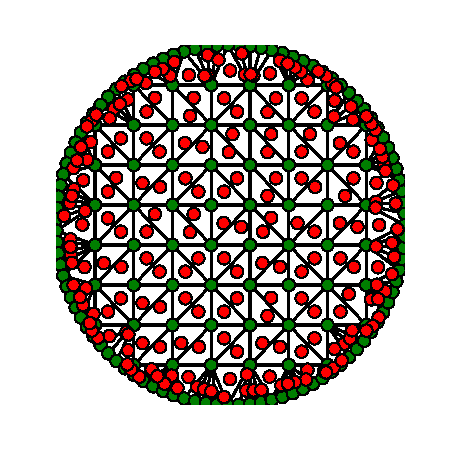
\includegraphics{figs/backmatter/meshCircle-100.pdf}
	\caption[Typical Delaunay triangulation mesh]
			{A typical mesh produced by the Delaunay triangulation.
			Here, 100 points were distrubuted along the boundary,  
			with another 100 inside the perimeter of the cavity. The green
			dots represent the nodes of the mesh. The red dots are the centroids
			of each triangle.}
	\label{fig:app.numMethods.meshDelaunayCircle}
\end{figure}

Figures \ref{fig:app.numMethods.fields} shows the field intensity
inside the cavity when $\phi(\bo{r})=J_0(kn_0r)$, i.e. the only
eigenfunction with vanishing angular momentum. We see that field
maintains its main features when a finer mesh is used, indicative
of the convergence of the method. 

\begin{figure}
	\centering
	\begin{subfigure}{0.47\textwidth}
		\centering
		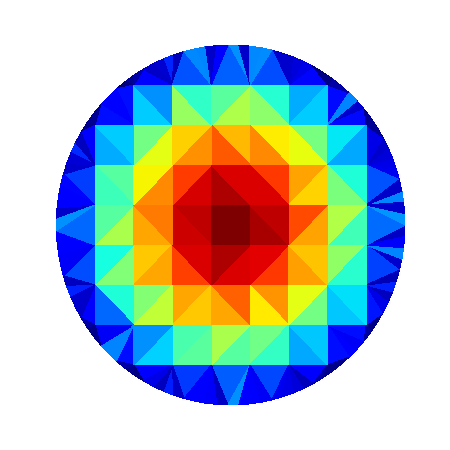
\includegraphics[width=\textwidth]{figs/backmatter/intensityTest-100.pdf}
		\caption[Intensity of the field inside the cavity]
				{Intensity of the field inside the cavity when
				$J_0(n_0kr)$ is the incoming field. This mesh contains
				100 points on the boundary and 100 more inside the perimeter.}
		\label{fig:app.numMethods.field.100}
	\end{subfigure}
	\hfill
	\begin{subfigure}{0.47\textwidth}
		\centering
		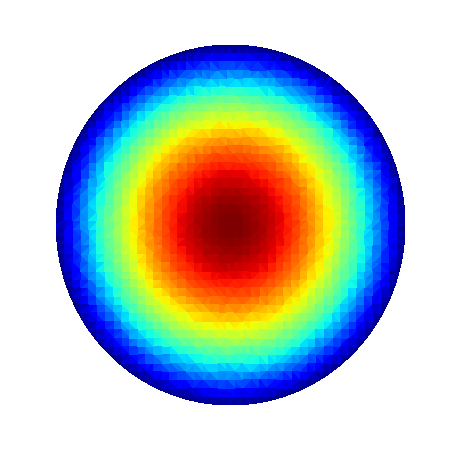
\includegraphics[width=\textwidth]{figs/backmatter/intensityTest-2000.pdf}
		\caption[Intensity of the field inside the cavity, finer mesh]
				{Intensity of the field inside the cavity when
				$J_0(kn_0r)$ is the incoming field. This mesh contains
				2000 points on the boundary and 2000 more inside the perimeter.}
		\label{fig:app.numMethods.field.2000}
	\end{subfigure}
	\caption[Intensity of the field inside the cavity for two different meshes]
			{Intensity of the field inside the cavity for two different meshes.
			We use $\phi(\bo{r})=J_0(kn_0r)$ as the incoming field.}
	\label{fig:app.numMethods.fields}
\end{figure}

The convergence is confirmed to be linear in the average area in 
the triangles in Figure \ref{fig:app.numMethods.convergenceIntegralMethod}.
The fact that it is slightly slower than linear can probably be 
attributed to the fact that we have neglected the diagonal 
parts of the kernel. 

\begin{figure}
	\centering
	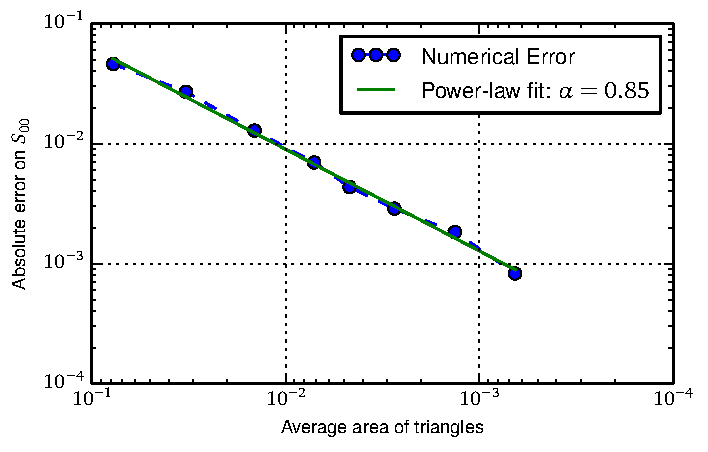
\includegraphics{figs/backmatter/convergenceAnalysis.pdf}
	\caption[Convergence analysis of the integral method]
			{Convergence analysis of the integral method. 
			We compute the difference between the analytical
			and numerical values of $S_{00}(k)$ for the homogeneous,
			circular cavity. The parameters are $k=1$, $R_0=1$, $n_c=1.5$
			and $n_0=1$.}
	\label{fig:app.numMethods.convergenceIntegralMethod}
\end{figure}

\section{Lippmann-Schwinger Copmputation of the Scattering Matrix: Vector Case}
We repeat the procedure of the previous section, but for the complete 3D vector
field. Similar methods are presented in \cite{deL2013,FAL2013}. As always, 
our starting point is the couple
	\begin{align}
		\nabla\times\bo{E}	& =ik\mu\bo{H}	& \nabla\times\bo{H}	&=-ik\epsilon\bo{E}.
	\end{align}
Taking the curl of the first equation and going through the motions, 
we can obtain the equation
	\begin{align}
		\label{eq:app.numMethods.LS.inhomogeneousPDE}
		\nabla^2\bo{E}+k^2\epsilon_\text{B}\mu_\text{B}\bo{E}	&=	-k^2\mu_\text{B}\Delta\epsilon\bo{E}
																	+\nabla\left\{\frac{1}{\epsilon_c}\bo{E}\cdot\nabla\epsilon_c\right\}	
																	+\mu_\text{B}\nabla\times\left(\Delta\mu^{-1}\nabla\times\bo{E}\right)
	\end{align}
where $\mu_\text{B}$ and $\epsilon_\text{B}$ are the permeability and permittivity
of the environment and where the supports of the functions
	\begin{align}
		\Delta\epsilon &= \epsilon_c-\epsilon_\text{B}	&	\Delta\mu^{-1}	&=\mu_c^{-1}-\mu_\text{B}^{-1}
	\end{align}
are supposed to coincide with the cavity region $\mathcal{C}$, 
with, now, $\mathcal{C}\subset\mathbb{R}^3$. $\epsilon_c$ 
and $\mu_c$ are the physical parameters of the cavity 
region and allowed to be non-linear, position- and frequency-dependent.
Once again, we have to solve an inhomogeneous partial differential equation.
We will use the tensorial Green's function\footnote{In the literature, it is called a dyadic 
Green's function. This nomenclature is archaic and should not be used in 
modern texts.}, given by \cite{NOV2012}
	\begin{equation}
		\mat{G}(\bo{r}',\bo{r}') = -\mat{I}\frac{e^{ikn_\text{B}|\bo{r}-\bo{r}'|}}{4\pi|\bo{r}-\bo{r}'|}.
	\end{equation}
where $n_B=\sqrt{\epsilon_B\mu_B}$. We can thus write a formal solution 
to the scattering problem as
	\begin{equation}
		\bo{E}(\bo{r}) = \bo{E}^i(\bo{r})
						+\mathop{\iiint}_\mathcal{C}\mat{G}(\bo{r},\bo{r}')\left[V(\bo{r}')\bo{E}(\bo{r}')\right]d^3\bo{r}'
	\end{equation}
where we have written the r.h.s. of \eqref{eq:app.numMethods.LS.inhomogeneousPDE}
as the operator
	\begin{equation}
		V(\bo{r}) = -k^2\mu_B\Delta\epsilon\left\{\right\}
					+\nabla\left\{\frac{1}{\epsilon_c}\left\{\right\}\cdot\nabla\epsilon_c\right\}
					+\mu_B\nabla\times\left(\Delta\mu^{-1}\nabla\times\left\{\right\}\right).
	\end{equation}
Once again, this Lippmann-Schwinger equation can be used to compute the scattering tensor
of the problem. If we use the eigenfunction as the incoming field, we have
	\begin{equation}
		\bo{E}(\bo{r}) = j_L(n_Bkr)\bo{Y}^L_{JM}(\theta,\varphi)
						+\mathop{\iiint}_\mathcal{C}\mat{G}(\bo{r},\bo{r}')\left[V(\bo{r}')\bo{E}(\bo{r}')\right]d^3\bo{r}'
	\end{equation}
where the vector spherical harmonics are given by a combination of the
scalar spherical harmonics
	\begin{equation}
		\bo{Y}^\ell_{jm} = \sum_{m'}\sum_{\sigma}C^{jm}_{lm',1\sigma}Y_\ell^{m'}(\theta,\varphi)\bou{e}_\sigma
	\end{equation}
where $C^{j_3m_3}_{j_1m_1,j_2m_2}$ are the Clebsch-Gordan coefficients and where
the $\bou{e}_\sigma$ are the unit vectors of the covariant spherical coordinate system \cite{VAR1988}.
We will use the expansion
	\begin{align}
		\mat{G}(\bo{r},\bo{r}')	&= -ik\sum_{j,\ell,m} j_\ell(n_Bkr_<)h^{(+)}_\ell(n_Bkr_>)
													\bo{Y}^{\ell}_{jm}(\theta,\varphi)\otimes\bo{Y}^{\ell*}_{jm}(\theta',\varphi').
	\end{align}
Using the same technique as before, i.e. substituting the expansion in the integral equation
for the field outside the \gls{lss} and invoking the definition of the scattering matrix, 
we obtain
	\begin{equation}
		S_{j\ell m,JLM} = \delta_{j\ell m,JLM}
			-2ik\mathop{\iiint}_\mathcal{C}j_\ell(kn_Br')\bo{Y}^{j*}_{\ell m}V(\bo{r}')\bo{E}(\bo{r}')d^3\bo{r}'.
	\end{equation}
To compute the scattering tensor, however, we must necessarily solve an integro-differential equation.
We will not delve into the subject, as it is beyond the scope of this essay. However, 
it could be solved via a Galerkin method. 

The curl-curl equation yields a simple integral method when the material
is non-magnetic, but it seems impossible to recover our simple expression
for the scattering tensor.
% !TeX root = ../msc_thesis_jayd.tex
\chapter{Numerical Tools}

\section{Numerical Computation of the Scattering Matrix in \gls{sqa}}\label{sec:app.numTools.scatMat}
We detail the numerical solution of Helmholtz's equation with the onion discretization 
procedure of \gls{sqa}.

In the TE case, we must take $n\mapsto n_\text{eff}$. This leads us to evaluate the 
extra integral
  \begin{equation}
   I = \frac{1}{2\pi}\int_0^{2\pi}\left[\frac{1}{n}\frac{d^2n(r_j,\theta)}{d\theta^2}-\frac{2}{n^2}\left(\frac{dn(r_j,\theta)}{d\theta}\right)^2\right]e^{i(m-m')\theta}d\theta.
  \end{equation}
The numerical cost of this integral can be lessened 
if we notice that if we write it as a function of $n^2$ we obtain
  \begin{equation}
   I = \frac{1}{2\pi}\int_0^{2\pi}\left[\frac{1}{2n^2}\frac{d^2n^2(r_j,\theta)}{d\theta^2}-\frac{3}{4n^4}\left(\frac{dn^2(r_j,\theta)}{d\theta}\right)^2\right]e^{i(m-m')\theta}d\theta
  \end{equation}
which, in turn, can be rewritten as
  \begin{equation}
   I = \frac{1}{2\pi}\int_0^{2\pi}\left[\frac{1}{2}\frac{d^2\log n^2(r_j,\theta)}{d\theta^2}-\left(\frac{1}{2}\frac{d\log n^2(r_j,\theta)}{d\theta}\right)^2\right]e^{i(m-m')\theta}d\theta.
  \end{equation}
Integrating by parts twice yields
  \begin{equation}
   I = \frac{1}{2\pi}\int_0^{2\pi}\left[-\frac{(m-m')^2}{2}\log n^2(r_j,\theta)-\left(\frac{1}{2}\frac{d\log n^2(r_j,\theta)}{d\theta}\right)^2\right]e^{i(m-m')\theta}d\theta.
  \end{equation}
The second term cannot be integrated out, but this final result means that
we will only need to numerically evaluate the first derivative of the 
refractive index (although its analytical form could be provided).

Notice the form of the $\mat{L}^j$ matrix. As can be seem from inspection, 
the value of the elements depend only on their distance from the diagonal.
Taking a closer look reveals the form
  \begin{equation}
   \mat{L}^j = \mat{M}^2 +k^2r_j^2\begin{pmatrix} 
		  n_0 & n_{-1} & \cdots & \cdots & n_{-2M}	\\
		  n_1	  & n_0& \cdots & \cdots & n_{-2M-1}\\
		  n_2	  & n_1	   & n_0& \cdots & n_{-2M-2}\\
		  \vdots  & n_2    & n_1    & \ddots & \vdots   \\
		  n_{2M}  & \cdots & \cdots & \cdots & n_0
		\end{pmatrix}
  \end{equation}
which is manifestly Toeplitz. When the potential is real, the Fourier
series has the property $n_{-j}=n_j^*$, which makes the $\mat{L}^j$ 
matrix Hermitian. In the general case, however, it is not. Because
we will need to use orthogonality relations in what follows, we must
compute both the left and right eigenvectors\index{left eigenvectors}. 
We will note the left (covariant) basis by $\Ket{\tilde{\Phi}_\mu^j}$.
This is not sufficient, however, because we are not guaranteed that
both sets of eigenvectors will form a complete basis. 

\paragraph{Normality of $\mat{L}^j$}

\section{Vector Scattering and the Variable Phase Method}\label{sec:app.numTools.vpm}
The \gls{vpm} is based upon an eigenfunction expansion of the 
angular part of the scattering equations. This reduces \gls{pde}
to a matrix \gls{ode} for the scattering amplitudes. In what
follows, we will derive those matrix \glspl{ode} for both 
2D scalar and 3D vector scattering. 

\subsection{2D Scalar Scattering}
Before applying the expansions, we will multiply the equation through 
by $n$ and write the derivatives explicitly
  \begin{equation}
    \left[n\left(\frac{\partial^2}{\partial r^2}+\frac{1}{r}\frac{\partial}{\partial r}+\frac{1}{r^2}\frac{\partial^2}{\partial\theta^2}\right)+k^2n^3\right]H_z
    =
    2\frac{\partial H_z}{\partial r}\frac{\partial n}{\partial r}+\frac{2}{r^2}\frac{\partial H_z}{\partial\theta}\frac{\partial n}{\partial\theta}.
  \end{equation}
Expanding this equation yields (after some simplification)
  \begin{multline}
   \sum_{m,m'}
    \left\{\frac{n_{m'}}{2\pi}\left(\frac{\psi_{m}''}{r^{1/2}}-\frac{(m^2-1/4)}{r^{5/2}}\psi_m\right)e^{i(m+m')\theta}\right\}
	+\left(\frac{k}{2\pi}\right)^2\left(\sum_{m'}n_{m'}e^{im'\theta}\right)^3\left(\sum_m\frac{\psi_m}{r^{1/2}}e^{im\theta}\right)\\
	=\frac{2}{2\pi}\sum_{m,m'}\left\{n_{m'}'\left[\frac{\psi_m'}{r^{1/2}}-\frac{\psi_m}{2r^{3/2}}\right]-\frac{mm'}{r^2}\frac{\psi_mn_{m'}}{r^{1/2}}\right\}e^{i(m+m')\theta}
  \end{multline}
Projecting onto $\sqrt{r}e^{-im''\theta}/\sqrt{2\pi}$
  \begin{multline}
    \sum_{m,m'}\int_0^{2\pi}\left\{\frac{n_{m'}}{(2\pi)^{3/2}}\left(\psi_m''-\frac{(m^2-1/4)\psi_m}{r^2}\right)+\frac{k^2c_{m'}\psi_m}{(2\pi)^{3/2}}\right\}e^{i(m+m'-m'')\theta}d\theta\\
    \frac{2}{(2\pi)^{3/2}}\int_0^{2\pi}\left\{n_{m'}'\left[\psi_m'-\frac{\psi_m}{2r}\right]-\frac{mm'}{r^2}\psi_mn_{m'}\right\}e^{i(m+m'-m'')\theta}d\theta
  \end{multline}
where
  \begin{equation}
   c_{m'} = \sum_{m}\sum_{m''}n_mn_{m''}n_{m'-m''-m}.
  \end{equation}
Integrating, introducing the matrices
  \begin{subequations}
  \begin{align}
   \left[\mat{N}(r)\right]_{mm''}	&= \sum_{m'}n_{m'}\delta_{m+m',m''}	\\
   \left[\mat{Z}(r)\right]_{mm''}	&= \sum_{m'}mm'n_{m'}'\delta_{m+m',m''},
  \end{align}
  \end{subequations}
we obtain the matrix ODE
  \begin{equation}
  \label{eq:vpm.TE.GeneralCase}
  \bo{\psi}''-\frac{\mat{M^2}-\mat{I}/4}{r^2}\bo{\psi}+\frac{k^2}{2\pi}\mat{N}^2\bo{\psi}
    =
   2\mat{N}^{-1}\mat{N}'\left[\bo{\psi}'-\frac{\psi}{2r}\right]-\frac{2}{r^2}\mat{N}^{-1}\mat{Z}\bo{\psi}
  \end{equation}
In the free case, i.e. $n(r,\theta)=1$, we have that
  \begin{equation}
   n_{m'} = \sqrt{2\pi}\delta_{m'0}
  \end{equation}
such that we have
  \begin{equation}
    \label{eq:vpm.freeCase}
    \bo{\psi}''-\frac{\mat{M}^2-\mat{I}/4}{r^2}\bo{\psi}+k^2\bo{\psi}=0,
  \end{equation}
the Bessel equation. For the general case, it makes sense
to posit a matrix solution of the form
  \begin{equation}
   \bo{\psi}=\mat{G}_k(r)\mat{W}(kr)
  \end{equation}
where $\left[\mat{W}(kr)\right]_{mm}=H_m^{(\pm)}(kr)$ where
we choose the sign for either incoming or outgoing 
wave boundary condition. Substituting this into \eqref{eq:vpm.TE.GeneralCase}
and using \eqref{eq:vpm.freeCase} gives
  \begin{multline}
    \label{eq:vpm.masterEquation}
    \mat{G}''+2\mat{G}'\frac{d}{dr}\left(\log\mat{W}\right)+\frac{1}{r^2}\left[\mat{G},\mat{M^2}-\mat{I}/4\right]+\frac{k^2}{2\pi}\left(\mat{N}^2-2\pi\right)
     \\ =
    2\mat{N}^{-1}\mat{N}'\left[\mat{G}'+\mat{G}\frac{d}{dr}\left(\log\mat{W}\right)-\frac{\mat{G}}{2r}\right]-\frac{2}{r^2}\mat{N}^{-1}\mat{ZG}.
  \end{multline}
In the case of TM polarization, the right-hand side 
of \eqref{eq:vpm.masterEquation} vanishes. 

We start with the matrix case. We parametrize the solution as
  \begin{equation}
    \mat{F}_k(r) = \mat{G}_k(r)\mat{W}(kr)
  \end{equation}
where $\mat{W}(kr)$ has the outgoing wave functions $rh_\ell^{(+)}(kr)$ on its diagonal. 
With the Sommerfeld condition, we can conclude that $\mat{G}_k(\infty) = \mat{I}$ and 
$\mat{G}_k'(\infty)=\mat{0}$. We have the differential equation
  \begin{multline}
   -\mat{G}_k(r)''-2\mat{G}_k(r)'\left(\frac{\partial}{\partial r}\ln\mat{W}(kr)\right)
    +\frac{1}{r^2}\left[\mat{L}^2,\mat{G}_k(r)\right]+\mat{V}(r)\mat{G}_k(r)=0
  \end{multline}
The incoming wave solutions solves the same equation, but with
$\mat{W}(kr)\mapsto \mat{W}(kr)^\dagger$. Denoting this solution 
by $\mat{G}_{-k}(r)$, we find that the wave function is
  \begin{equation}
    \bo{\psi}(r) = \mat{G}_{-k}(r)\mat{W}(kr)^\dagger+\mat{G}_k(r)\mat{W}(kr)\mat{S}_k(k)
  \end{equation}
where $\mat{S}_k(k)$ is the scattering matrix. Because of the
$1/r$ factor in our expansion, $\bo{\psi}(0)$ must vanish 
for the field to be finite at the origin. We can then write the 
scattering matrix as
  \begin{equation}
   \mat{S}_k = -\lim_{r\rightarrow0}\mat{W}^{-1}(kr)\mat{G}^{-1}_k(r)\mat{G}_{-k}(r)\mat{W}(kr)^\dagger
  \end{equation}
These equations come from \cite{FOR2012}, modulo some minor changes.

Not surprisingly, we will have to deal with exactly the same issue as before: 
notice the product $\mat{W}^\dagger(kr)\mat{A}\mat{W}^{-1}(kr)$. For diagonal
matrices $\mat{W}$, we can rewrite this product as
  \begin{equation*}
    \mat{A}\circ\left(\text{diag}(\mat{W}^\dagger)\otimes\text{diag}(\mat{W}^{-1})\right)
  \end{equation*}
which is our beloved Schur product that caused some issues in \gls{sqa}. 

\subsection{3D Vector Scattering}
In the electromagnetic case, we start with the curl-curl equation
  \begin{equation}
    \nabla\times\nabla\times\bo{E}-k^2\epsilon(\bo{r})\bo{E}=0.
  \end{equation}
Expanding the field in a tensor spherical harmonics (to be discussed later) yields
an implicit differential equation. In their paper, F+G argue that if they rather
use the equation
  \begin{equation}
   \label{eq:vpm.modCurlCurl}
   \nabla\times\nabla\times\bo{E}(\bo{r})-\epsilon(\bo{r})\nabla\left\{\nabla\cdot\left[\epsilon(\bo{r})\bo{E}(\bo{r})\right]\right\}
      =k^2\epsilon(\bo{r})\bo{E}(\bo{r})
  \end{equation}
which yields the same eigenstates, the resulting differential equation is explicit. 
Interestingly enough, this is exactly the extra term that is used to remove
spurious solutions that appear in variational treatments. 

Recall that we can write Maxwell's equations as the minimization of the energy-like functional
  \begin{equation}
   F\left[\bo{E}\right]=\mathop{\iiint}_V\left[\left(\nabla\times\bo{E}^*\right)\left(\nabla\times\bo{E}\right)-k^2\bo{E}^*\cdot\epsilon(\bo{r})\bo{E}\right]dV.
  \end{equation}
In the variational treatment, this leads to spurious solutions which can provably be removed \cite{KON1976,KOS1984,KOS1985} that adding the null term
$\left(\nabla\cdot\bo{E}^*\right)\left(\nabla\cdot\epsilon(\bo{r})\bo{E}\right)$ in the integrand. 
Taking the first variation of the new functional leads to \eqref{eq:vpm.modCurlCurl}.
  
We now expand both the permittivity $\epsilon(\bo{r})$ and the field in
spherical harmonics. Because the electric field is a vector field, 
we will need to use \textit{vector} spherical harmonics, given by
  \begin{equation}
    \bo{Y}_{jm}^\ell=\sum_{\sigma=-1}^{+1}\sum_{m'=\ell}^{+\ell}C^{jm}_{\ell m'1\sigma}Y_{\ell}^{m'}(\theta,\varphi)\bou{e}_\sigma
  \end{equation}
where $\ell=j,j\pm1$ for the three vector spherical harmonics, $C^{nm}_{n_1m_1,n_2m_2}$
is a Clebsch-Gordan coefficient and the spherical basis vectors $\bou{e}_\sigma$ 
are
  \begin{align}
    \bou{e}_1	&= -\frac{e^{i\varphi}}{\sqrt{2}}\left(\sin\theta\bou{r}+\cos\theta\bou{\theta}+i\bou{\varphi}\right)	\nonumber\\
    \bou{e}_0	&= \cos\theta\bou{r}-\sin\theta\bou{\theta}								\\
    \bou{e}_{-1}&= -\bou{e}_1^*												\nonumber
  \end{align}
Before going any further, let us state the capabilities of this approach. This kind of method
can theoretically deal with arbitrary potentials (permittivities). However, it is best used
when the scale of variations of the potential is not too big compared to the size
of the scatterer. The size of the transforms and matrix ODEs, or in other words the resolution
must be fixed beforehand. For fast variations of the potential, a smaller resolution must be used
and this leads to overall large matrices. For highly non-uniform structures, finite element methods
might be preferable. Radial inhomogeneities can be dealt with variable-step integrators. 
Magnetic materials can be considered by substituting the curl-curl operator $\nabla\times\nabla\cdots$
by $\nabla\times\frac{1}{\mu(\bo{r})}\nabla\times\cdots$. 

\section{Lippmann-Schwinger Computation of the Scattering Matrix}\label{sec:app.numTools.lippmannSchwinger}
\section{Computation of the Logarithmic Derivative $[H^{(\pm)}_\nu(z)]'/H^{(\pm)}_\nu(z)$}\label{sec:app.numTools.logDeriv}

\index{continued fraction expansions|(textbf}
As we have seen from Appendix \ref{sec:app.basicEquationScattering}, the computation of the logarithmic derivative
of Bessel functions is of the utmost importance in the numerical solution 
of scattering problems. Given that we already use Amos' library \cite{AMO86} to evaluate
the Bessel functions, we might have been tempted to use it 
to directly evaluate the derivative. It turns out that using
expansions that pertain to logarithmic derivatives is somewhat
faster and is more accurate than using Amos' library. 

In this section, we introduce some concepts relating to 
continued fraction expansions (CFEs) and discuss their numerical
evaluation. We then derive the CFEs and other expansions that will
be of use in the computation of the logarithmic derivatives.

\subsection{Notation and Necessary Theorems}
A continued fraction expansion is a representation
of a mathemetical function. It can be linked to 
Laurent series, Padé approximants and much more 
\cite{CUY2008}. It has the standard form 
  \begin{equation}
    f = b_0+\cfrac{a_1}{b_1+\cfrac{a_2}{b_2+\cfrac{a_3}{b_3+\cfrac{a_4}{b_4+\cdots}}}}
  \end{equation}
or, more succinctly, 
  \begin{equation}
   f = b_0 + \bigk_{m=1}^\infty\left(\frac{a_m}{b_m}\right)
  \end{equation}
where 'K' is for the German word \textit{Kettenbruch}, meaning continued fraction.
We define the $n$th approximant as
  \begin{equation}
   f_n = b_0 + \bigk_{m=1}^n\left(\frac{a_m}{b_m}\right).
  \end{equation}
We will be concerned with their numerical evaluation and convergence properties.

\index{continued fraction expansions!numerical evaluation of}
Notice that naïvely evaluating the CFE from right-to-left, as a person would do, 
does not yield a satisfying numerical algorithm, as the amount of iterations 
must be fixed in advance and consequently does not allow the control the 
accuracy of the evaluation. The chosen method is taken from the Holy Bible
of Numerics, \textit{Numerical Recipes} \cite{PRE2007} and is called 
the modified Lentz's method. It constructs a rational approximation
of the $n$th approximant 
  \begin{equation}
    f_n = \frac{A_n}{B_n}
  \end{equation}
where 
  \begin{align}
   A_{-1} 	&=1 			& B_{-1} 	&=0	\nonumber\\
   A_0		&= b_0			& B_0		&=1	\\
   A_j		&=b_jA_{j-1}+a_jA_{j-2}	& B_j 		&=b_jB_{j-1}+a_jB_{j-2}.\nonumber
  \end{align}
This method can lead to over/underflow of the floating-point representation: 
the method hence uses 
  \begin{align}
    C_j &= A_j/A_{j-1}			&	D_j	&= B_{j-1}/B_j	\nonumber\\
    	&= b_j+\frac{a_j}{C_{j-1}}	&		&= \frac{1}{b_j+a_jD_{j-1}}\\
    f_j	&= f_{j-1}C_jD_j.\nonumber
  \end{align}
The method is aptly described by Algorithm \ref{algo:app.numTools.cfeEvaluation}.
It allows for a left-to-right evaluation of the CFE and control of the relative
accuracy of the computation. 

  \begin{algorithm}
   \KwData{\texttt{tiny} = square root of smallest representable number}
   \KwData{\texttt{eps} = accuracy of the CFE}
   \eIf{$b_0 = 0$}{$f_0\leftarrow$\texttt{tiny}}{$f_0\leftarrow0$}
   $C_0 \leftarrow f_0$\;
   $D_0 \leftarrow 0$\;
   \Repeat( from $j=1$){$|\Delta_j-1|<$\texttt{eps}}%
   {
    $D_j \leftarrow b_j+a_jD_{j-1}$\;
    \If{$D_j=0$}{$D_j\leftarrow$\texttt{tiny}}
    $C_j \leftarrow b_j+\frac{a_j}{C_{j-1}}$\;
    \If{$C_j=0$}{$C_j\leftarrow$\texttt{tiny}}
    $D_j \leftarrow 1/D_j$\;
    $\Delta_j\leftarrow C_jD_j$\;
    $f_j \leftarrow f_{j-1}\Delta_j$
   }
   \Return{$f_j$}
  \caption{Evaluation of Continued Fractions}
  \label{algo:app.numTools.cfeEvaluation}
  \end{algorithm}

As for the convergence properties, we will only bother with CFEs 
originating from three-term recurrence relations. Indeed, it turns out
that any three-term recurrence relation can be linked to a CFE. 
Consider  
  \begin{equation}
    \label{eq:app.numTools.threeTermRecurrence}
   y_{n+1} + a_ny_n + b_ny_{n-1} = 0. 
  \end{equation}
It can be rewritten as
  \begin{equation}
    \frac{y_n}{y_{n-1}} = -\frac{b_n}{a_n+y_{n+1}/y_n}.
  \end{equation}
Iterating yields the CFE
  \begin{equation}
   \label{eq:app.numTools.recurrenceCFE}
   \frac{y_n}{y_{n-1}} = \bigk_{m=n}^\infty\left(\frac{-b_m}{a_m}\right).
  \end{equation}
Given our goal of computing $[H^{(\pm)}_\nu(z)]'/H^{(\pm)}_\nu(z)$
and in light of (ref to recurrence relation of Bessel functions), it seems that
we have won. The next theorem, however, will prove us wrong.
   \begin{thm}[Pincherle's Theorem \cite{CUY2008}]
    If there exists a \textit{minimal solution} $u_n$ of the three-term
    recurrence relation \eqref{eq:app.numTools.threeTermRecurrence}, 
    the associated CFE \eqref{eq:app.numTools.recurrenceCFE} converges
    to $u_n/u_{n-1}$. A solution is said minimal if there exists another
    solution $v_n$ such that
      \begin{equation}
       \lim_{n\rightarrow\infty} \frac{u_n}{v_n} = 0.
      \end{equation}
    $v_n$ is said to be the dominant solution. The minimal solution is unique. 
   \end{thm}

Because the minimal solution of \eqref{eq:app.Bessel.recurrenceBessel} if $J_\nu(z)$, 
we cannot use the associated CFE to compute the logarithmic derivatives
of Hankel functions. Instead, we must look into the links between
Hankel functions and confluent hypergeometric functions. 

\subsection{CFE and Other Expansions}
In this brief foray into the vast subject
of hypergeometric functions, we will introduce Kummer's 
function and its link to the evaluation of the logarithmic
derivative.

Kummer's function solves the differential equation \cite[\S13.1.1]{ABR1965}
  \begin{equation}
    z\frac{d^2y}{dz^2}+(b-z)\frac{dy}{dz}-ay=0
  \end{equation}
and is noted $U(a,b,z)$. It can be shown that that $u_k=(a)_kU(a+k,b,z)$
is the minimal solution of the recurrence \cite{TEM1983}
  \begin{equation}
    u_{n+1} = \frac{2a-b+2n+z}{a-b+n+1}u_n - \frac{a+n-1}{a-b+n+1}u_{n-1}
  \end{equation}
where $(a)_k$ is the Pochhammer symbol. We can hence derive
  \begin{equation}
    \frac{U(a,b,z)}{U(a+1,b,z)} = 2a-b+2+z-\bigk_{m=1}^\infty\left(\frac{(a+m)(b-a-m-1)}{b-2a-2m-2-z}\right).
  \end{equation}
Combined with \cite[\S13.4.23]{ABR1965}
  \begin{equation}
    U(a+1,b,z) = \frac{1}{1+a-b}U(a,b,z) + \frac{z}{a(1+a-b)}U'(a,b,z), 
  \end{equation}
we obtain \cite{CUY2008}
  \begin{equation}
    \frac{dU(a,b,z)/dz}{U(a,b,z)} = -\frac{a}{z}+\frac{a(1+a-b)/z}{2a-b+2+z}_{-}\bigk_{m=1}^\infty\left(\frac{(a+m)(b-a-m-1)}{b-2a-2m-2-z}\right).
  \end{equation}
Given the relation between Kummer's functions and Hankel functions $H^\omega_{\nu}(z)$ \cite[\S13.6.22/23]{ABR1965}
  \begin{equation}
    H^\omega_\nu(z) = \frac{2}{\sqrt{\pi}}e^{-\omega\left[\pi\left(\nu+1/2\right)-z\right]}(2z)^\nu U(\nu+1/2,2\nu+1,-2i\omega z)\qquad (\omega=\pm)
  \end{equation}
we can finally find the CFE
  \begin{equation}
    \label{eq:app.numTools.cfeHankel}
    \frac{dH^\omega_\nu(z)/dz}{H^\omega_\nu(z)} = -\frac{1}{2z}+i\omega+\frac{\omega}{z}\bigk_{m=1}^\infty\left(\frac{\nu^2-(2m-1)^2/4}{2(iz-\omega m)}\right).
  \end{equation}
In our numerical implementation (see next section), we have found that when $|z|<10^{-2}$, convergence is slow. This mirrors the results of \cite{THO1986}.
We thus use the small argument expansions for the Bessel functions (\textit{q.v.} \S \ref{sec:app.Bessel.smallArguments}) to obtain
  \begin{subequations}
  \begin{align}
   \lim_{z\rightarrow0}\frac{dH^\omega_\nu(z)/dz}{H^\omega_\nu(z)}	&= -\frac{\nu}{z}	& (\nu\neq0)	\\
									&= \frac{1}{z}\left[\frac{\pi}{2i\omega}+\gamma+\ln\left(\frac{z}{2}\right)\right]^{-1} & (\nu=0).
  \end{align}
  \end{subequations}

\index{continued fraction expansions|)textbf}

\subsection{Numerical Tests}
We have performed a number of tests to ascertain the performance of our algorithm. 
To test the precision of the algorithm, we have evaluated the CFE for $z\in\{0,10\}$
and $\nu\in\{-100,100\}\in\mathbb{N}$ and compared it to the values obtained via
Amos' library for a range of tolerances. It can be seen that the maximum deviation 
decreases until our set tolerance hits $10^{-12}$ and then plateaus. Because 
convergence of \ref{eq:app.numTools.cfeHankel} is mathematically insured, we 
conclude that Amos's library evaluate the logarithmic derivative up to 
a precision of $10^{-12}$. This is probably due to the propagation 
of errors in the floating point operations, as we use relation
\eqref{eq:app.Bessel.recurrenceDiffBessel}
to evaluate the derivative. 

\begin{figure}
 \centering
 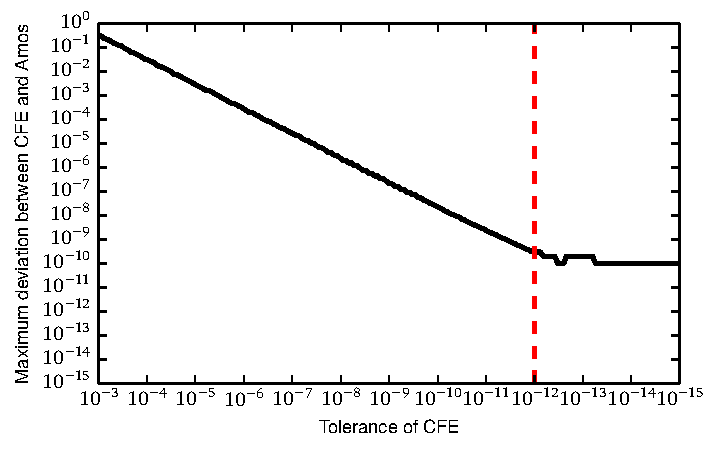
\includegraphics[width=0.7\textwidth]{figs/app-numTools/maxDiff.pdf}
 \caption[Maximum deviation between the CFE and Amos' implementation as a function
	  of the CFE tolerance]%
	 {Maximum deviation between the CFE and Amos' implementation of the Bessel functions
	 as a function of the tolerance of the CFE. This study was performed in the parameter
	 space $z\in\left\{0.1,10\right\}, \nu\in\left\{-100,100\right\}$. We interpret 
	 the plateau in maximum deviation as the error committed by Amos' implementation, i.e.
	 Amos' implementation has a precision of $\sim10^{-10}$ on the evaluation of the logarithmic derivative.}
\end{figure}


\begin{figure}
 \centering
 \begin{subfigure}[t]{0.47\textwidth}
  \centering
  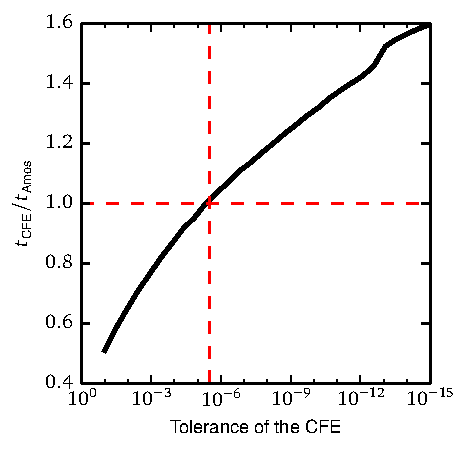
\includegraphics[width=\textwidth]{figs/app-numTools/timesTolerance.pdf}
  \caption{Performance of the CFE implementation as a function of its tolerance.
	   We measured the ratio of the time it takes to compute the logarithmic derivative
	   at $z=0$ for all orders $\nu\in\{-100,100\}$ with the CFE and Amos' implementation. 
	   When the tolerance of the CFE hits $\sim10^{-5.5}$, the CFE is slower than Amos'
	   implementation.}
 \end{subfigure}
 \begin{subfigure}[t]{0.47\textwidth}
  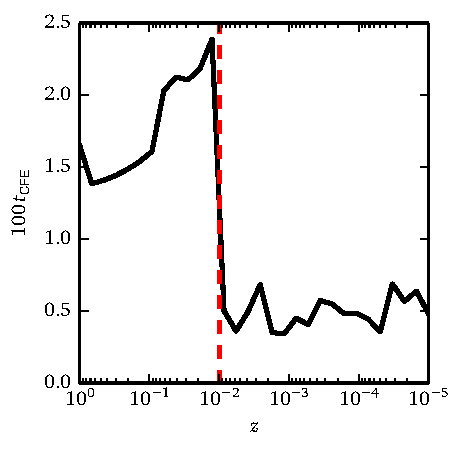
\includegraphics[width=\textwidth]{figs/app-numTools/timesPerformance.pdf}
  \caption{Performance of the CFE as a function of $z$. When approaching
  $z=0$ (from all sides), it takes a higher number of terms for the 
  CFE to converge, resulting in a slower algorithm. However, at $z=10^{-2}$, we 
  use the small argument form, preserving both precision and performance.}
 \end{subfigure}
 \caption[Performance of the CFE compared to Amos' library's.]
	 {Performance of the CFE compared to that of Amos' library. The CFE is somewhat
	 slower, but can achieve better precision.}
\end{figure}


However, it can be seen that Amos' library is somewhat faster, given its
precision, that our CFE evaluation 
even though it requires three Hankel function evaluations. 

%\section{Clebsch-Gordan Coefficients and Wigner Symbols}
\section{Wigner Symbols}\label{sec:app.wignerSymbols}
Before discussing the Wigner symbols, we introduce the Clebsch-Gordan
coefficients as they appear quite naturally in the quantum theory
of angular momentum. Specifically, they are needed to study the coupling
of two systems having definite angular momenta. The material in this section
is inspired by \cite{VAR1988,BRI1993}. 

\subsection{Formal definitions}
\subsubsection{Clebsch-Gordan coefficients and Wigner $3j$-symbols}
Given two states that can be described by two quantum numbers
pertaining to their angular momenta, say $\ket{j_1m_1}$
and $\ket{j_2m_2}$ where $j_1$ and $j_2$ are the total
angular momenta and $m_1$ and $m_2$ are their $z$-projections. 
The states span two different vectors spaces, $\xi_1$ and $\xi_2$. 
To measure the angular momentum and associated $z$-projection
of the composite system, call them $j_3$ and $m_3$, we look at
the states spanning the product space $\xi_1\otimes\xi_2$. The product
states can be written
  \begin{equation}
   \ket{j_3m_3} = \sum_{m_1}\sum_{m_2}\ket{j_1m_1j_2m_2}\braket{j_1m_1j_2m_2|j_3m_3}
  \end{equation}
where
  \begin{equation*}
   \ket{j_1m_1j_2m_2}=\ket{j_1m_1}\otimes\ket{j_2m_2}
  \end{equation*}
and where the allowed values of $j_3$ and $m_3$ follow 
from the quantum vector addition rules. 

A similar relation holds for the bra. This equation simply 
describes the expansion of the a vector in the product space
$\xi_1\otimes\xi_2$ in the product of the bases of $\xi_1$ 
and $\xi_2$ \cite{COH1973b}. The expansion coefficients are known as the 
Clebsch-Gordan coefficients. Their square represent 
the probability that a measurement of the angular momentum 
yields a value of $\sqrt{j_3(j_3+1)}\hbar$.

We will note the Clebsch-Gordan coefficients
as
  \begin{equation}
    C^{j_3m_3}_{j_1m_1,j_2m_2} = \braket{j_1m_1j_2m_2|j_3m_3}.
  \end{equation}

We can now introduce the Wigner $3j$-symbols. They can be related
to the Clebsch-Gordan coefficients through
  \begin{equation}
   \begin{pmatrix} j_1 & j_2 & j_3 \\
		   m_1 & m_2 & m_3
   \end{pmatrix}
    = \frac{(-1)^{j_1-j_2-m_3}}{\sqrt{2j_3+1}}\braket{j_1m_1j_2m_2|j_3-m_3}.
  \end{equation}
More telling, though, is their interpretation as the probability
that three angular momenta couple to give zero angular momentum, or
  \begin{equation}
   \begin{pmatrix} j_1 & j_2 & j_3 \\
		   m_1 & m_2 & m_3
   \end{pmatrix}
    = (-1)^{j_1-j_2+j_3}\sum_{j'm'} C^{j'm'}_{j_1m_1,j_2m_2}C^{00}_{j'm',j_3m_3}.
  \end{equation}
The $3j$-symbols also appear in the angular integration of three spherical
harmonics 
  \begin{equation}
    \mathop{\iint}_\Omega Y_{j_1,m_1}(\theta,\varphi)Y_{j_2,m_2}(\theta,\varphi)Y_{j_3,m_3}(\theta,\varphi)d\Omega
      =
    \sqrt{\frac{(2j_1+1)(2j_2+1)(2j_3+1)}{4\pi}}\begin{pmatrix} j_1 & j_2 & j_3 \\ 0 & 0 & 0 \end{pmatrix}\begin{pmatrix} j_1 & j_2 & j_3 \\ m_1 & m_2 & m_3\end{pmatrix}
  \end{equation}

\subsubsection{Wigner $6j$-symbols}
The $6j$-symbols are related to the coupling of three angular momenta. In
this case, the resultant angular momentum $\bo{j}$ can be obtained via three 
different coupling schemes:
  \begin{enumerate}[I.]
   \item $\bo{j}_1+\bo{j_2}=\bo{j}_{12}, \qquad \bo{j}_{12}+\bo{j}_3=\bo{j}$;
   \item $\bo{j}_2+\bo{j_3}=\bo{j}_{23}, \qquad \bo{j}_1+\bo{j}_{23}=\bo{j}$;
   \item $\bo{j}_1+\bo{j_3}=\bo{j}_{13}, \qquad \bo{j}_{13}+\bo{j}_2=\bo{j}$.
  \end{enumerate}
Each coupling scheme has a set of associated \textit{generalized Clebsch-Gordan}
coefficients which gives the coefficients of the expansion of a state vector
in the basis of $\ket{j_1m_1,j_2m_2,j_3m_3}$. For instance, a state 
corresponding to coupling scheme I has expansion
  \begin{equation}
   \ket{j_1j_2(j_{12}),j_3jm} = \sum_{m_1,m_2,m_3}C_{j_{12}m_{12}j_3m_3}^{jm}C_{j_1m_1j_2m_2}^{j_{12}m_{12}}\ket{j_1m_1,j_2m_2,j_3m_3}
  \end{equation}
with similar expressions holding for the other coupling schemes.

We thus define the $6j$-symbols as the coefficients of the unitary
transformation that takes us from one scheme to another \cite{VAR1988}.
We can then write
  \begin{equation}
   \begin{Bmatrix} j_1 & j_2 & j_3 \\ j_4 & j_5 & j_6 \end{Bmatrix} = \frac{(-1)^{j_1+j_2+j_4+j_5}}{\sqrt{(2j_3+1)(2j_6+1)}}
      \sum_{m_1,m_2,m_3,m_4,m_6} C_{j_3m_3,j_4m_4}^{j_5m_5}C_{j_1m_1,j_2m_2}^{j_3m_3}C_{j_1m_1,j_6m_6}^{j_5m_5}C_{j_2m_2,j_4m_4}^{j_6m_6}
  \end{equation}


We can also define higher-order Wigner symbols, but things rapidly become complicated \cite{YUT1962}. 

\subsection{Numerical Computation of Wigner Symbols}
The previous section dealt with the definitions of 
the Clebsch-Gordan coefficients and the Wigner symbols. 
While more (much, much more) could have been said on the
subject, we will now discuss the actual evaluation of these
numbers. 

We note that the Condon-Shortley phase convention 
assures us all Clebsch-Gordan coefficients and 
Wigner symbols are real, which is a real numerical
advantage. 

Moreover, there exists closed-forms formulas in the form of algebraic
sums for the Wigner symbols, but they are riddled with numerical 
issues, such as the cancellation of large terms and the evaluation 
of the ratio of large factorial arguments. 

The best way to evaluate the coefficient was devised in 1975
by chemical physicist K. Schulten \cite{SCH1975}. 
He and R. G. Gordon 
rederived three-term recursion relation for the Wigner symbols 
and used them to evaluate sets of Wigner symbols at a time.
Fortran 
code exists\footnote{\url{http://cpc.cs.qub.ac.uk/summaries/ACWQ_v1_0.html}}, 
but our tests showed only \texttt{single} numerical precision. We have
thus reprogrammed the algorithm, first described in \cite{SCH1975}
and detailed in \cite{SCH1976}, in C++. 

Before detailing our results, we will briefly overview
the algorithm used (\see Figure \ref{fig:app.wigner.flowchart}. We compute
  \begin{align*}
    \begin{pmatrix}j_1 & j_2 & j_3 \\ m_1 & m_2 & m_3 \end{pmatrix} \qquad \forall j_1 \\
    \begin{Bmatrix}j_1 & j_2 & j_3 \\ j_4 & j_5 & j_6 \end{Bmatrix} \qquad \forall j_1
  \end{align*}
We can write the recursion relations valid for both symbols as 
(we adopt the notation of \cite{LUS1998})
  \begin{equation}
    \alpha_\psi(j_1)\psi(j_1+1)+\beta_\psi(j_1)\psi(j_1)+\gamma_\psi(j_1)\psi(j_1-1)=0
  \end{equation}
where $\psi(j_1)$ represents either the $3j$- or $6j$-symbol at $j_1$
and the Greek letters are the coefficient at that $j_1$. They are
shown in Table \ref{tab:app.wigner.coeffsRecursion}. 

To start the recursion, we would usually need two initial
conditions. It turns out, however, that the recursion
relations reduce to only two terms at the boundaries
$j_{1\text{min}}$ and $j_{1\text{max}}$. Like all
other numerical schemes, recursion relations
are only stable in the direction of increasing
coupling coefficients. Semi-classical analysis
\cite{SCH1975} informs us that there generally exists
three regions of interest for the function $\psi(j_1)$.
Near the boundaries, we are in the nonclassical 
regions. At the lower values of $j_1$, $\psi(j_1)$
is increasing until it hits the central classical
region, where it starts oscillating. On the other
hand, near the $j_{1\text{max}}$ boundaries, the
coefficients are increasing with decreasing $j_1$. 
Given the linearity of the recursion relations, we
can start the recursion relations from both boundaries
using a sufficiently small but otherwise \textit{arbitrary} number. 
While the ratios between successive values of the coupling coefficients
will be correct, their absolute values will not. The forward and backward
recurrences will be multiplied by a scalar, call them $c_1$ for the forward
recursion and $d_1$ for the backward recursion. To find the relationship
between the scalars, we watch the values of the forward and backward
recursions at some intermediary point. For more numerical stability, 
we use three contiguous values around the intermediary point
and find the parameter $\lambda=\nicefrac{d_1}{c_1}$ from a least-squares fit.
To choose the intermediary point, we note that the recursion relations
appear in the form
  \begin{equation}
   \psi(j_1+1)=X(j_1)\psi(j_1)+Y(j_1)\psi(j_1-1).
  \end{equation}
Schulten found that, using semiclassical analysis, 
that $|X(j_1)|$ attains its minimum value 
in the classical domain. Monitoring the variation
of $|X(j_1)|$ thus provides a way to find the intermediary point.

The overall scaling factor $c_1$ is found and the set of 
coupling coefficients is rescaled to its proper value
by using the normalization condition on the computed set.

We note that if the total size of the set is 1 ($j_{1\text{min}}=j_{1\text{max}}$), 
we can deduce, from the triangular condition, that $l_2\lor l_3=0$. We thus have
to evaluate the $3j$-symbols 
  \begin{align*}
   \begin{pmatrix} l_3 & 0 & l_3 \\ -m_3 & 0 & m_3 \end{pmatrix} &= \begin{pmatrix} l_3 & l_3 & 0 \\ m_3 & -m_3 & 0\end{pmatrix}=\frac{(-1)^{l_3-m_3}}{\sqrt{2l_3+1}}	\\
   \begin{pmatrix} l_2 & l_2 & 0 \\ -m_2 & m_2 & 0 \end{pmatrix} &= (-1)^{-2l_2}\begin{pmatrix} l_2 & l_2 & 0 \\ m_2 & -m_2 & 0\end{pmatrix}\\&=\frac{(-1)^{-l_2-m_3}}{\sqrt{2l_2+1}}
  \end{align*}
When the size is 2, we simply the two-term recursion formula with an arbitrary 
initial condition and normalize the two coefficients obtained. 

\begin{figure}
 \centering
 \begin{subfigure}[b]{0.5\textwidth}
  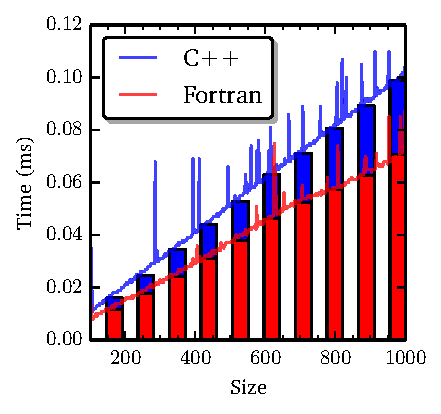
\includegraphics[width=\textwidth]{figs/backmatter/wignerTimes.pdf}
  \caption{Time (in ms) to compute sets of a given size of coupling coefficients, specifically the 
	    $3j$-symbol, in this case.}
 \end{subfigure}\hfill
 \begin{subfigure}[b]{0.5\textwidth}
  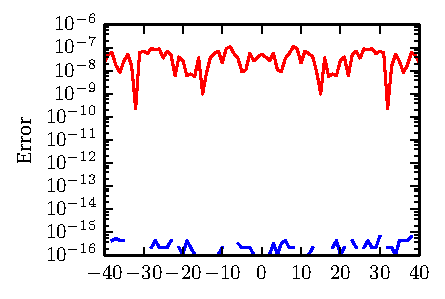
\includegraphics[width=\textwidth]{figs/backmatter/wignerPrecision.pdf}
  \caption{Precision of the Fortran and C++ implementations of the algorithm obtained%
	    by computing the orthogonality relationship \eqref{eq:app.wigner.orthogonality}.}
 \end{subfigure}
 \caption{Performance and precision of our numerical algorithms.}
\end{figure}

\begin{equation}
 \label{eq:app.wigner.orthogonality}
 \sum_{m1,m2} (2l_3+1)\begin{pmatrix} l_1 & l_2 & l_3 \\ m_1 & m_2 & m_3\end{pmatrix}^2=1
\end{equation}


\begin{table}
 \begin{center}
 \newcommand{\A}{$\begin{aligned}A(j_1) &=\left[j_1^2-(j_2-j_3)^2\right]^{1/2}\\&\phantom{=}\times\left[(j_2+j_3+1)^2-j_1^2\right]^{1/2}\\&\phantom{=}\times\left[j_1^2-m_1^2\right]^{1/2}\end{aligned}$}
 \newcommand{\B}{$\begin{aligned}B(j_1) &=-(2j_1+1)\\&\phantom{=}\times\left[j_2(j_2+1)m_1\right.\\&\phantom{=\times}-j_3(j_3+1)m_1\\&\phantom{=\times}\left.-j_1(j_1+1)(m_3-m_2)\right]\end{aligned}$}
 \newcommand{\E}{$\begin{aligned}E(j_1) &=\left\{\left[j_1^2-(j_2-j_3)^2\right]\right.\\&\phantom{=}\times\left[(j_2+j_3+1)^2-j_1^2\right]\\&\phantom{=}\times\left[j_1^2-(j_5-j_6)^2\right]\\&\phantom{=}\times\left.\left[(j_5+j_6+1)^2-j_1^2\right]\right\}^{1/2}\end{aligned}$}
 \newcommand{\F}{$\begin{aligned}F(j_1) &= (2j_1+1)\\&\phantom{=}\times\left\{j_1(j_1+1)\left[--+\right]\right.\\&\phantom{=\times}+j_5(j_5+1)\left[++-\right]\\&\phantom{=\times}+j_6(j_6+1)\left[+-+\right]\\&\phantom{=\times}\left.-2j_1(j_1+1)l_1(l_1+1)\right\}\end{aligned}$}
 \caption{Parameters and coefficients of the three-term recursion relations satisfied
	  by the $3j$- and $6j$-symbols.
	  The expression $[++-]$ represents the coefficient $[j_1(j_1+1)+j_2(j_2+1)-j_3(j_3+1)]$ and similarly for other signs in the bracket.}
 \label{tab:app.wigner.coeffsRecursion}
  \begin{tabular*}{\columnwidth}{m{0.1\textwidth}@{\extracolsep{\fill}}l@{\extracolsep{\fill}}l}
  \hline\hline
  $3j$- or $6j$-symbols	&	 $f(j_1)=\begin{pmatrix} j_1 & j_2 & j_3 \\ m_1 & m_2 & m_3 \end{pmatrix}$ & $h(j_1)=\begin{Bmatrix} j_1 & j_2 & j_3 \\ j_4 & j_5 & j_6 \end{Bmatrix}$\\
  \hline
  $\alpha_\psi$			& $j_1A(j_1+1)$		& $jE(j_1+1)$	\\
  $\beta_\psi$			& $B(j_1)$		& $F(j)$	\\
  $\gamma_\psi$			& $(j_1+1)A(j_1)$	& $(j_1+1)E(j)$	\\
				&			&		\\
  \multirow{4}{*}{Functions}	& \A			& \E		\\
  				&			&		\\
				& \B			& \F		\\
				&			&		\\
 \multirow{2}{*}{Endpoints}	& $j_{1\text{min}}=\text{max}(|j_2-j_3|,|m_1|)$ & $j_{1\text{min}}=\text{max}(|j_2-j_3|,|j_5-j_6|)$	\\
				& $j_{1\text{max}}=j_2+j_3$ 			& $j_{1\text{max}}=\text{min}(j_2+j_3,j_5+j_6)$		\\
				&			&		\\
 Normalization			& $\sum_{j_1}(2j_1+1)f(j_1)^2=1$		& $(2j_4+1)\sum_{j_1}(2j_1+1)h(j_1)^2=1$		\\
 				&			&		\\
 Sign				& $\text{sgn}[f(j_{1\text{max}})]=(-1)^{j_2-j_3-m_1}$ & $\text{sgn}[h(j_{1\text{max}})]=(-1)^{j_2+j_3+j_5+j_6}$\\
  \hline\hline
 \end{tabular*}
 \end{center}
\end{table}


% -- We draw a flowchart of the algorithm. 
% Block styles
\tikzstyle{decision} = [diamond, draw, fill=blue!20,text width=4.5em, text badly centered, node distance=3cm, inner sep=0pt]
\tikzstyle{block} = [rectangle, draw, fill=blue!20, text width=5em, text centered, rounded corners, minimum height=4em]
\tikzstyle{line} = [draw, -latex']
\tikzstyle{cloud} = [draw, ellipse,fill=red!20, node distance=3cm,minimum height=2em]
\tikzstyle{empty} = [fill=white]

% Actual flowchart
\begin{figure}
\begin{center}
\begin{tikzpicture}[scale=0.75,node distance = 2.8cm, auto]
 % -- We place the nodes
 \node [block] (init) {Enforce selection rules};
 \node [decision, below of=init] (sizeSets) {Determine boundaries and size of set};
 \node [block, below of=sizeSets] (size2) {Two-term forward recursion};
 \node [block, left of=size2] (size1) {Use analytical formula};
 \node [block, right of=size2] (otherSize) {Forward recursion};
 \node [decision,below of=otherSize] (overflow){$|\psi(j_1)|>$\\SRHUGE?};
 \node [block, left of=overflow](rescale) {Rescale forward recursion};
 \node [decision,below of=overflow] (monitor) {$|X(j_1)|$ increasing?};
 \node [decision,below of=monitor] (loopDone) {Loop done?};
 \node [block,left of=loopDone] (backward) {Backward recursion until midpoint};
 \node [block,below of=backward] (lambda) {Compute $\lambda$; rescale forward recursion};
 \node [block,right of=lambda] (normalization) {Normalize set of coefficients};
 \node [block, below of=normalization] (return){Return};
 
 % -- We place the edges
 \path [line] (init) -- (sizeSets);
 \path [line] (sizeSets) -| node [near end] {size$=1$} (size1);
 \path [line] (sizeSets) -- node [near start] {size$=2$} (size2);
 \path [line] (sizeSets) -| node [near end] {other sizes} (otherSize);
 \path [line] (otherSize) -- (overflow);
 \path [line] (overflow) -- node[near start]{yes} (rescale);
 \path [line] (overflow) -- node[near start]{no}  (monitor);
 \path [line] (rescale) |- (monitor);
 \path [line] (monitor.south west) -- node[near start]{yes} (backward.north east);
 \path [line] (monitor) -- node[near start]{no} (loopDone);
 \path [line] (loopDone.east) -- node[near start]{no} ($(loopDone.east)+(2,0)$) |- (otherSize.east);
 \path [line] (loopDone) -- node[near start]{yes} (normalization);
 \path [line] (normalization) -- (return);
 \path [line] (backward) -- (lambda);
 \path [line] (lambda) -- (normalization);
 \path [line] (size1) |- (return);
 \path [line] (size2.south) -- ($(size2.south)-(0,1)$) -- ++(-2,0) -- ($(lambda.south)-(2,1)$) -- ++(3,0) -- (normalization.south west);
\end{tikzpicture}
\end{center}
\caption{Flowchart of the algorithm used to compute the coupling coefficients. SRHUGE is the 
	  square root of the biggest representable number in our floating point representation.}
\label{fig:app.wigner.flowchart}
\end{figure}

\section{Spherical Harmonics Transform}
In the variable phase method, we must find the spherical 
harmonics transform, i.e. the spherical moments, of the 
potential. To find these moments, we will have to become
intimate with the spherical harmonics. 

\subsection{Definition of the scalar and vector spherical harmonics}
While there is a number of ways to introduce the spherical harmonics, 
we will take the top to bottom approach: from the general to the specific. 
In all generality, spherical harmonics are solutions of the equation
  \begin{equation}
    \left[\nabla^2_\Omega+\ell(\ell+1)\right]Y^{\ell S}_{jm}(\theta,\varphi)=0
  \end{equation}
where $Y_{jm}^{\ell S}$ is actually a \textit{tensor} spherical harmonic. 
It describes the angular distribution and polarization of spin-$S$ particles 
with angular momentum $j$, projection $m$ and orbital angular momentum $\ell$ \cite{VAR1988}.
While the study of particles with arbitrary spin $S$ is interesting in its own right,
we will concentrate on the case of particles of spin-$1$ and their scalar approximation
(spin-$0$). Since the values of $\ell$ range from $|J-S|$ to $J+S$, the 
spin-$0$ case reduces to the usual scalar spherical harmonics while the spin-$1$
case are the \textit{vector} spherical harmonics. As said in the main text, they 
can be formed by a superposition of scalar spherical harmonics of the form
  \begin{equation}
    \bo{Y}_{jm}^\ell(\theta,\varphi)=\sum_{m',\sigma}C_{lm',1\sigma}^{jm}Y_\ell^{m'}(\theta,\varphi)\hat{\bo{e}}_\sigma
  \end{equation}
The numerical evaluation of these functions are then contingent on the evaluation of the
scalar spherical harmonics and the Clebsch-Gordan coefficients. The first was covered in the 
previous appendix and we will soon tend to the second. 

The scalar spherical harmonics can simply be written as
  \begin{equation}
   Y_{\ell}^m(\theta,\varphi) = P_\ell^m(\cos\theta)e^{im\varphi}
  \end{equation}
where $P_\ell^m$ is the normalized version of the associated 
Legendre polynomials \cite{PRE2007}. They are related to
the usual Legendre polynomials $\widetilde{P}_\ell^m$ through
  \begin{equation}
    P_\ell^m(x) = \sqrt{\frac{2\ell+1}{4\pi}\frac{(\ell-m)!}{(\ell+m)!}}\widetilde{P}_\ell^m(x)
  \end{equation}
To numerically evaluate the spherical harmonics, then, we must safely 
evaluate the associated Legendre polynomials. One of the only 
stable recurrence relation is \cite{PRE2007}
  
  \begin{equation}
   P_\ell^m(x)=\sqrt{\frac{4l^2-1}{l^2-m^2}}\left[xP_{\ell-1}^m(x)-\sqrt{\frac{(l-1)^2-m^2)}{4(l-1)^2-1}}P_{\ell-2}^m(x)\right]
  \end{equation}
The initial conditions are provided by 
  \begin{align}
   P_m^m(x)	&=(-1)^m\sqrt{\frac{2m+1}{4\pi(2m)!}}(2m-1)!!(1-x^2)^{m/2}	\\
   P_{m+1}^m(x)	&=x\sqrt{2m+3}P_m^m(x)
  \end{align}
At first sight, it might seem dangerous to evaluate 
$P_m^m(x)$ because of the division of two factorial functions. 
However, by taking the square of the expression and looking
at the factorial functions, we have
  \begin{equation}
   a_m = \frac{[(2m-1)!!]^2}{(2m)!}.
  \end{equation}
This can evaluated rather simply by noting that $(2m-1)!!=\nicefrac{(2m)!}{2^mm!}$.
Rearranging, we get
  \begin{equation*}
   a_m = \frac{(2m)!}{2^{2m}(m!)^2} = \frac{1}{2^{2m}}\binom{2m}{m}.
  \end{equation*}
We further notice that
  \begin{equation}
   \frac{a_{m+1}}{a_m} = \frac{2^{2m}}{2^{2(m+1)}}\frac{\binom{2(m+1)}{m+1}}{\binom{2m}{m}}=\frac{2m+1}{2m+2}.
  \end{equation}
We can then safely evaluate $P_m^m(x)$ using the formula
  \begin{equation}
   P_m^m(x) = \sqrt{\frac{2m+1}{4\pi}\prod_{i=0}^{m-1}\frac{2i+1}{2i+2}(1-x^2)}.
  \end{equation}

Our numerical implementation shows machine precision for all spherical
harmonics up to $\ell=3$ (we compared the results of our algorithm 
with the analytical forms of the spherical harmonics).  Moreover, we 
tested our algorithm against the following sums \cite[\S 5.10]{VAR1988}
  \begin{align}
   \sum_{m} \left|Y_\ell^m(\theta,\varphi)\right|^2	&= \frac{2\ell+1}{4\pi}	\label{eq:app.sph.sum1}\\
   \sum_m m\left|Y_\ell^m(\theta,\varphi)\right|^2 	&= 0			\label{eq:app.sph.sum2}\\
   \sum_m m^2\left|Y_\ell^m(\theta,\varphi)\right|^2	&= \frac{\ell(\ell+1)(2\ell+1)}{8\pi}\sin^2\theta.\label{eq:app.sph.sum3}
  \end{align}
They are verified to a precision of $10^{-7}$ up to $\ell=500$. The uncertainty
on the sums grows with $\ell$. Figure \ref{fig:app.sph.precision} tells us 
that the spherical harmonics are computed near to or at machine precision
(in \texttt{double}). The increasing error is due to error accumulation. 
At large $\ell$, there are a lot of terms to sum, thus increasing
the absolute error made in the computation. 

\subsection{Spherical Harmonics Transform}
While the Fast Fourier Transform has had hundreds
of experts working on it, this is not true of the 
Fast Spherical Harmonics Transform. The program libraries
are scarce and, for the most part, still in their infancy. 
This is in sharp contrast with the FFT case, where numerous 
libraries provide algorithms that performs FFTs at a cost 
of $\mathcal{O}(n\log n)$. \texttt{FFTW} is an example of such a mature, 
robust program library.

Any smooth function can be expanded in a spherical harmonics
series (they form a complete basis on the 2-sphere) with \cite[\S 6.7.1]{PRE2007}
  \begin{equation}
    f(\theta,\varphi) = \sum_{\ell=0}^{\ell_\text{max}}\sum_{m=-\ell}^\ell a_{\ell m}P_\ell^m(\cos\theta)e^{im\varphi}
  \end{equation}
Using the orthonormality conditions, we can find an expression for the expansion coefficients
  \begin{equation}
   a_{\ell m} = \mathop{\iint}_\Omega f(\theta,\varphi)e^{-im\varphi}P_\ell^m(\cos\theta)\sin\theta d\theta d\varphi
  \end{equation}
In the discrete case, then, the integral becomes a quadrature
  \begin{equation}
   a_{\ell m} = \sum_{i,j}w(\theta_i)f(\theta_i,\varphi_j)e^{-im\varphi_j}P_\ell^m(\cos\theta_i).
  \end{equation}
The fastest way to perform the quadrature over $\varphi_j$ is, of course, to use
the FFT. We will perform the quadrature over $\theta_i$ by using a Gauss-Legendre
quadrature. While the cost of such an algorithm is the worst we could get ($\mathcal{O}(\ell^3)$), 
it is also the easiest to implement. Faster transforms are available in the literature \cite{TYG2006,TYG2008,TYG2010}.

To find the abscissas of the Gauss-Legendre quadrature (the roots
of $P_\ell^0(\cos\theta)$), we perform a few rounds of Newton-Raphson 
using the following initial guess on the positions of the zeros \cite{ABR1965}
  \begin{equation}
   \xi_{\ell,k} = \left(1-\frac{1}{8\ell^2}+\frac{1}{8\ell^3}\right)\cos\left(\frac{4k-1}{4\ell+2}\pi\right)+\mathcal{O}\left(\ell^{-4}\right)
  \end{equation}
where $\xi_{\ell,k}$ is the $k$th root (ordered in $[-1,1]$) of $P_\ell^0(\cos\theta)$.

\begin{figure}
 \centering
 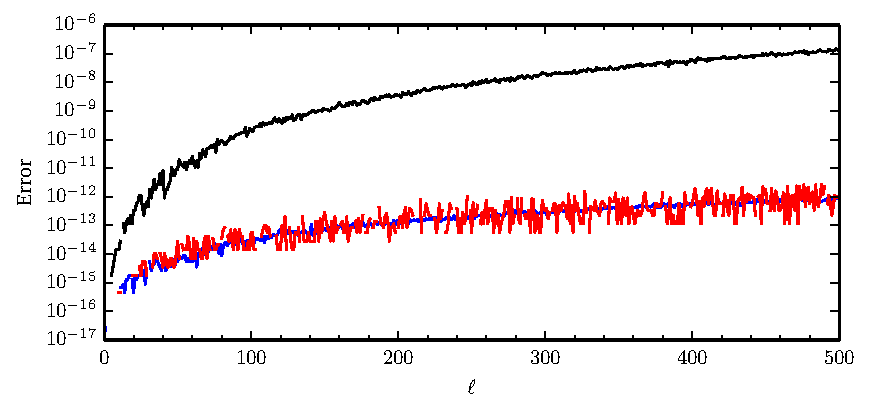
\includegraphics[width=0.9\textwidth]{figs/backmatter/SphPrecision.pdf}
 \caption[Precision of our implementation of the algorithm that evaluates the spherical harmonics]
	  {Precision of our implementation of the algorithm that evaluates the spherical harmonics. 
	  The {\color{blue} blue} curve corresponds to \eqref{eq:app.sph.sum1}, the 
	  {\color{red} red} curve to \eqref{eq:app.sph.sum2} and the black curve to 
	  \eqref{eq:app.sph.sum3}.}
 \label{fig:app.sph.precision}
\end{figure}

 \nocite{*}

\bibliographystyle{osajnl}
\bibliography{memoir_jayd}

\printindex

\end{document}